%% ut-thesis.tex -- document template for graduate theses at UofT
%%
%% Copyright (c) 1998-2013 Francois Pitt <fpitt@cs.utoronto.ca>
%% last updated at 16:20 (EDT) on Wed 25 Sep 2013
%%
%% This work may be distributed and/or modified under the conditions of
%% the LaTeX Project Public License, either version 1.3c of this license
%% or (at your option) any later version.
%% The latest version of this license is in
%%     http://www.latex-project.org/lppl.txt
%% and version 1.3c or later is part of all distributions of LaTeX
%% version 2005/12/01 or later.
%%
%% This work has the LPPL maintenance status "maintained".
%%
%% The Current Maintainer of this work is
%% Francois Pitt <fpitt@cs.utoronto.ca>.
%%
%% This work consists of the files listed in the accompanying README.

%% SUMMARY OF FEATURES:
%%
%% All environments, commands, and options provided by the `ut-thesis'
%% class will be described below, at the point where they should appear
%% in the document.  See the file `ut-thesis.cls' for more details.
%%
%% To explicitly set the pagestyle of any blank page inserted with
%% \cleardoublepage, use one of \clearemptydoublepage,
%% \clearplaindoublepage, \clearthesisdoublepage, or
%% \clearstandarddoublepage (to use the style currently in effect).
%%
%% For single-spaced quotes or quotations, use the `longquote' and
%% `longquotation' environments.


%%%%%%%%%%%%         PREAMBLE         %%%%%%%%%%%%

%%  - Default settings format a final copy (single-sided, normal
%%    margins, one-and-a-half-spaced with single-spaced notes).
%%  - For a rough copy (double-sided, normal margins, double-spaced,
%%    with the word "DRAFT" printed at each corner of every page), use
%%    the `draft' option.
%%  - The default global line spacing can be changed with one of the
%%    options `singlespaced', `onehalfspaced', or `doublespaced'.
%%  - Footnotes and marginal notes are all single-spaced by default, but
%%    can be made to have the same spacing as the rest of the document
%%    by using the option `standardspacednotes'.
%%  - The size of the margins can be changed with one of the options:
%%     . `narrowmargins' (1 1/4" left, 3/4" others),
%%     . `normalmargins' (1 1/4" left, 1" others),
%%     . `widemargins' (1 1/4" all),
%%     . `extrawidemargins' (1 1/2" all).
%%  - The pagestyle of "cleared" pages (empty pages inserted in
%%    two-sided documents to put the next page on the right-hand side)
%%    can be set with one of the options `cleardoublepagestyleempty',
%%    `cleardoublepagestyleplain', or `cleardoublepagestylestandard'.
%%  - Any other standard option for the `report' document class can be
%%    used to override the default or draft settings (such as `10pt',
%%    `11pt', `12pt'), and standard LaTeX packages can be used to
%%    further customize the layout and/or formatting of the document.

%% *** Add any desired options. ***
\documentclass{ut-thesis}
\usepackage{amsmath}
\usepackage{graphicx}
\usepackage{natbib}


%% *** Add \usepackage declarations here. ***
%% The standard packages `geometry' and `setspace' are already loaded by
%% `ut-thesis' -- see their documentation for details of the features
%% they provide.  In particular, you may use the \geometry command here
%% to adjust the margins if none of the ut-thesis options are suitable
%% (see the `geometry' package for details).  You may also use the
%% \setstretch command to set the line spacing to a value other than
%% single, one-and-a-half, or double spaced (see the `setspace' package
%% for details).


%%%%%%%%%%%%%%%%%%%%%%%%%%%%%%%%%%%%%%%%%%%%%%%%%%%%%%%%%%%%%%%%%%%%%%%%
%%                                                                    %%
%%                   ***   I M P O R T A N T   ***                    %%
%%                                                                    %%
%%  Fill in the following fields with the required information:       %%
%%   - \degree{...}       name of the degree obtained                 %%
%%   - \department{...}   name of the graduate department             %%
%%   - \gradyear{...}     year of graduation                          %%
%%   - \author{...}       name of the author                          %%
%%   - \title{...}        title of the thesis                         %%
%%%%%%%%%%%%%%%%%%%%%%%%%%%%%%%%%%%%%%%%%%%%%%%%%%%%%%%%%%%%%%%%%%%%%%%%

%% *** Change this example to appropriate values. ***
\degree{Doctor of Philosophy}
\department{Ecology and Evolutionary Biology}
\gradyear{2015}
\author{Emily Beth Josephs}
\title{The Evolutionary Genetics of Gene Expression in \textit{Capsella grandiflora}}

%% *** NOTE ***
%% Put here all other formatting commands that belong in the preamble.
%% In particular, you should put all of your \newcommand's,
%% \newenvironment's, \newtheorem's, etc. (in other words, all the
%% global definitions that you will need throughout your thesis) in a
%% separate file and use "\input{filename}" to input it here.


%% *** Adjust the following settings as desired. ***

%% List only down to subsections in the table of contents;
%% 0=chapter, 1=section, 2=subsection, 3=subsubsection, etc.
\setcounter{tocdepth}{2}

%% Make each page fill up the entire page.
%\flushbottom


%%%%%%%%%%%%      MAIN  DOCUMENT      %%%%%%%%%%%%

\begin{document}

%% This sets the page style and numbering for preliminary sections.
\begin{preliminary}

%% This generates the title page from the information given above.
\maketitle

%% There should be NOTHING between the title page and abstract.
%% However, if your document is two-sided and you want the abstract
%% _not_ to appear on the back of the title page, then uncomment the
%% following line.
\cleardoublepage

%% This generates the abstract page, with the line spacing adjusted
%% according to SGS guidelines.
\begin{abstract}
This is my abstract
%% *** Put your Abstract here. ***
%% (At most 150 words for M.Sc. or 350 words for Ph.D.)
\end{abstract}

%% Anything placed between the abstract and table of contents will
%% appear on a separate page since the abstract ends with \newpage and
%% the table of contents starts with \clearpage.  Use \cleardoublepage
%% for anything that you want to appear on a right-hand page.

%% This generates a "dedication" section, if needed -- just a paragraph
%% formatted flush right (uncomment to have it appear in the document).
\begin{dedication}
To my grandmothers, Myra Josephs and Mary Barnard.
\end{dedication}

%% The `dedication' and `acknowledgements' sections do not create new
%% pages so if you want the two sections to appear on separate pages,
%% uncomment the following line.
\newpage  % separate pages for dedication and acknowledgements

%% Alternatively, if you leave both on the same page, it is probably a
%% good idea to add a bit of extra vertical space in between the two --
%% for example, as follows (adjust as desired).
%\vspace{.5in}  % vertical space between dedication and acknowledgements

%% This generates an "acknowledgements" section, if needed
%% (uncomment to have it appear in the document).
\begin{acknowledgements}
%% *** Put your Acknowledgements here. ***
Here are my Acknowledgements. Thanks everybody!
\end{acknowledgements}

%% This generates the Table of Contents (on a separate page).
\tableofcontents

%% This generates the List of Tables (on a separate page), if needed
%% (uncomment to have it appear in the document).
\listoftables

%% This generates the List of Figures (on a separate page), if needed
%% (uncomment to have it appear in the document).
\listoffigures

%% You can add commands here to generate any other material that belongs
%% in the head matter (for example, List of Plates, Index of Symbols, or
%% List of Appendices).

%% End of the preliminary sections: reset page style and numbering.
\end{preliminary}


%%%%%%%%%%%%%%%%%%%%%%%%%%%%%%%%%%%%%%%%%%%%%%%%%%%%%%%%%%%%%%%%%%%%%%%%
%%  Put your Chapters here; the easiest way to do this is to keep     %%
%%  each chapter in a separate file and `\include' all the files.     %%
%%  Each chapter file should start with "\chapter{ChapterName}".      %%
%%  Note that using `\include' instead of `\input' will make each     %%
%%  chapter start on a new page, and allow you to format only parts   %%
%%  of your thesis at a time by using `\includeonly'.                 %%
%%%%%%%%%%%%%%%%%%%%%%%%%%%%%%%%%%%%%%%%%%%%%%%%%%%%%%%%%%%%%%%%%%%%%%%%

%% *** Include chapter files here. ***

\setlength{\parindent}{0ex}
\setlength{\parskip}{2ex}

\chapter{General introduction}

\say{No one supposes that all the individuals of the same species are cast in the very same mould. These individual differences are highly important for us, as they afford materials for natural selection to accumulate} 
\begin{flushright}
--- \citet{darwin1859}
\end{flushright}

\say{The individuals belonging to a species differ to a greater or less extent”} 
\begin{flushright}
--- \citet{haldane1932}
\end{flushright}

\say{Attempts to understand the causes and significance of organic diversity have been made ever since antiquity; the problem seems to possess an irresistible aesthetic appeal.} 
\begin{flushright}
--- \citet{dob1937}
\end{flushright}

\say{“There is a considerable amount of genic variation segregating in all of the populations studied and that the real variation in these populations must be greater than we are able to demonstrate.”}
\begin{flushright}
--- \citet{Lewontin1966-kz}
\end{flushright}

As many great evolutionary biologists have noted, natural variation is ubiquitous. However, the relative importance of various evolutionary forces in maintaining this variation, especially at the population level, is still unknown. 

\section{Population genetic approaches to the maintenance of variation.}

The question of what forces maintain genetic variation has been investigated extensively in population genetics. Two competing hypotheses formed early on for explaining within-population variation (reviewed in \citet{lewontin1974}). The “classic” school argued that little variation segregates in populations, most new mutations are deleterious, and most observed variation was transient, on the way to either adaptive fixation or removal. In contrast, the “balance” school argued that large amounts of genetic variation are maintained within populations due to heterosis or other forms of balancing selection. 

As the first protein polymorphism  data emerged, it appeared that neither hypothesis could explain the data \citep{Lewontin1966-kz,Harris1966-lm}. Levels of heterozygosity in proteins were too high to be explained by balancing selection alone since at every polymorphic allele, homozygotes will still make up at least 50\% of the population at Hardy-Weinberg equilibrium, leading to extreme variation in fitness between individuals and inbreeding depression \citep{lewontin1974}. However, high levels of sequence variation did not fit with the original classical theory’s prediction that there is low variation within populations. Kimura and Ohta reconciled high within-population variation with the classic school by proposing that most of the sequence variation observed in nature both within and between populations is either selectively neutral or effectively selectively neutral \citep{Kimura1968-cl,Mootoo_Kimura1971-dc,Kimura_undated-by,Ohta1973-qx}.

However, genome-wide sequence data has shown that selection does shape observed genetic variation and molecular divergence between species, both directly in coding and noncoding sequence, and indirectly through linked selection. McDonald-Kreitman based approaches have found that \textgreater 30\% of replacement fixations in \textit{Drosophila} and \textit{Escherichia coli} are due to positive selection \citep{Eyre-Walker2006-jg,Fay2002-au,Begun2007-gh}. Within population estimates of the distribution of fitness effects of segregating mutations show that weakly deleterious mutations contribute significantly to standing genetic variation in humans \citep{Williamson2005-ja,Eyre-Walker2006-tr}. 

There is also evidence that selection shapes genetic variation outside genic regions. \citet{Begun2007-gh} found constraint across intergenic, intronic, and untranslated regions of the \textit{D. simulans} genome and there is constraint in the noncoding sequences that flank genes of other species \citep{Eory2010-ja}. However, quantifying selection in noncoding regions is difficult because these regions do not break down into obvious selected and neutral sites. Methods that have used information about specific function have been able to detect selection on functional sites such as transcription factor binding sites \citep{Arbiza2013-te} and phylogenetically-conserved noncoding sequences \citep{Halligan2013-pz}. 

There is mounting evidence that selection shapes diversity at neutral sites in linkage disequilibrium with directly selected sites. Linked neutral diversity will be removed by both fixations due to positive selection \citep{Smith1974} and the removal of polymorphisms by negative selection \citep{Charlesworth1993-xx}. The combined effects of selective sweeps and background selection are widespread, as demonstrated by positive correlations between recombination rate and polymorphism \citep{Cutter2003-yq,Nachman1998-vc,Kim2007-ju,Begun2007-gh,Tenaillon2001-ai}, negative correlations between divergence and polymorphism \citep{Andolfatto2007-ew,Hahn2008-yj,Macpherson2007-pl}, and reduced average neutral diversity around replacement fixed substitutions relative to silent fixed substitutions \citep{Sattath2011-ns} but see \citep{hernandez2011}. Recent estimates suggest that linked selection dramatically reduces genome-wide diversity in the \textit{Drosophila simulans} genome \citep{Elyashiv2014-ic}.

Most of the discussion above focussed on negative and positive selection, which both remove genetic variation from within populations, but selection can also directly increase genetic variation through balancing selection. However, the impact of balancing selection on sequence variation has generally been difficult to quantify. Balancing selection can result from a number of different processes, including heterosis, frequency-dependent selection, spatially-variable selection, and temporally-variable selection \citep{Hedrick2006-ft,Hedrick1976-qp} and the temporal scale at which balancing selection occurs will affect the types of genetic signatures it leaves behind \citep{Charlesworth2006-mw}. For example, long-term balancing selection appears to maintain genetic variation between humans and chimpanzees at a number of loci \citep{Leffler2013-wr} but the genetic signature of short-term balancing selection is difficult to disentangle from other demographic events \citep{Charlesworth2006-mw}.

Overall, it is clear that some genetic variation is neutral, some is deleterious, and some is beneficial. However, the relative importance of these processes for shaping genome-wide variation is still unclear.

\section{Quantitative genetic approaches to the maintenance of variation}
The types of selection that shape sequence variation may differ from the types of selection that shape phenotypic variation because much of the variation at sequence level may not translate into phenotype (this is a central tenet of the nearly neutral theory). Since selection generally acts on the phenotype, understanding the selective forces that maintain genetic variation for phenotype is crucial. The main hypotheses for the maintenance of quantitative genetic variation for phenotypic traits mirror those in population genetics: mutation-selection balance and balancing selection \citep{N_H_Barton1989-yu,Johnson2005-dl}.

An exemplar of the kinds of approaches that quantitative geneticists have used to address the maintenance of genetic variation comes from Kelly, who proposed that the contribution of deleterious alleles to genetic variation could be quantified by investigating the directional dominance of variation in a trait \citep{Kelly1999-re}. Applications of this approach have shown that intermediate-frequency alleles, not rare recessive alleles as expected under mutation-selection balance, can explain variation for flower size in \textit{Mimulus guttatus} and female fecundity in \textit{Drosophila}. \citep{Kelly2001-rc,Charlesworth2007-rp} However, this approach requires multiple generations of breeding in order to measure directional dominance and has so far only been applied to a few traits that may not be representative of all traits. 

\section{Linking genotype and phenotype}
Developing an understanding of the selective forces that maintain genetic variation for phenotype on a systematic level will require linking genetic variation to phenotypic variation. An enormous effort has been made over the last few decades to do exactly this, using techniques like linkage mapping, quantitative trait loci mapping, and genome-wide association studies (GWAS). I will refer to all of these techniques under the umbrella term “QTN program”. following \citet{Rockman2012-ks}.

Often the QTN program has not been motivated by evolutionary questions, but instead by an attempt to better understand the molecular basis of a trait and then use this information to develop treatments for a disease, find genetic regions that could be introgressed into crop plants, or other practical uses. However, evolutionary biologists have also made use of QTN techniques to describe the genetic architecture of traits \citep{lynch1998}. It seems especially appealing to use the sample of known QTNs (sometimes distressingly referred to as the “QTLome” \citep{Martinez_undated-wg}) to make general conclusions about the types of variation maintained within populations \citep{Barton2002-do}.

Unfortunately, inferring the selective forces acting on variation from QTNs is not straightforward \citep{Rockman2012-ks,Johnson2005-dl}. The act of finding QTNs biases us towards finding large-effect alleles but other lines of evidence suggest that small-effect QTNs are also important for genetic variation. For example, the inability of genome-wide association mapping studies to identify large-effect common alleles for many heritable human diseases suggests that either small-effect and/or very rare large-effect alleles make up genetic variation for these traits (reviewed in Rockman 2012). 

As emphasized by \citep{Lee2014-pi}, identifying QTNs within a population is still a useful approach to understanding how selection acts on traits. Specifically, QTNs maintained by mutation-selection balance are expected to be maintained at low allele frequencies while QTNs maintained by balancing selection are expected to be maintained at intermediate allele frequencies \citep{Barton2002-do}. However, efforts to infer selective forces acting on QTNs must be careful of the ascertainment biases that filter the sample of known QTNs. One successful approach has been a set of studies that estimate the proportion of variation in a trait explained by all genotyped loci to show that small-effect alleles do contribute to genetic variation, even though the specific loci involved are unknown \citep{Yang2010-iu,International_Schizophrenia_Consortium2009-ks}.

A potential strategy for generating a sample of QTNs with relatively small fitness effects is to investigate the loci that affect gene expression. While expression is often thought of as an intermediate phenotype, it is more useful in this case to think of it as a ‘model phenotype’ that integrates across phenotypic space, is straightforward to measure on a large scale, and is measurable without prior, potentially biasing information about how a certain expression level may vary in nature or influence fitness \citep{Rockman2006-yx}.

\section{The importance of standing variation for adaptation}

While understanding the maintenance of variation is fundamental for a full understanding of evolutionary biology, it is also relevant because the types of variation maintained within populations will control adaptation. The classic theory predicts that adaptation occurs through new mutations, leading to the signatures of “classic” selective sweeps and an adaptive walk that occurs in short mutation-limited bursts \citep{Smith1974,Allen_Orr2005-fs,Fisher1930-el}. However, the balance theory suggests that ecologically relevant variation waits within populations, ready to contribute to adaptation if conditions change. Adaptive mutations that rise to fixation from standing variation will leave a subtler sweep signal in linked neutral variation since more than one haplotype may fix in the population \citep{pennings2006_2,pennings2006_3,hermisson2005}. If adaptation occurs at many loci present in standing variation, the population can reach a new trait optimum without any fixations at all \citep{Pritchard2010-uh,Pritchard2010-uq}.

The origin of adaptive alleles will not only affect our ability to detect that adaptation using population genetic data, but will also affect the kinds of mutations that actually fix during adaptation. For example, adaptation from standing variation may involve more small-effect alleles than adaptation from new mutation \citep{Orr2001-fq}. In addition, local adaptation between divergent populations from standing variation may involve more instances of conditional neutrality, where one allele is selected in one population and neutral in another population, than trade-offs, where alleles are alternately favored and disfavored in populations, since the alleles involved in trade-offs are less likely to be maintained within populations than neutral alleles \citep{Anderson2011-hs}. 

\section{Research Objectives}

Throughout the course of my Ph.D., I have investigated the selective forces that maintain genetic variation within populations and that shape sequence variation at the population, within-species, and between-species level. Below I describe my study system and outline the chapters of my thesis.

\subsection{Study System}
I used the species \textit{Capsella grandiflora} throughout my thesis. \textit{C. grandiflora} has been a useful system for the investigation of selective forces for a number of reasons. First, \textit{C. grandiflora} has had a large, relatively stable effective population size making both positive and negative selection strong relative to drift \citep{Slotte2010-gw}. Second, \textit{C. grandiflora} has relatively low population structure \citep{St_onge2011-jz}, making it possible to do population genomics on a species-wide sample and minimizing the impact that migration from nearby populations will have on a focal population. Third, unlike most plant model systems, \textit{C. grandiflora} is obligately outcrossing, making it appropriate for answering questions about selective forces that act within populations. Finally, \textit{C. grandiflora} is a highly tractable genomic system. It has a small genome for a plant (134 MB), making it feasible to generate and map sequence data from a population sample and is closely related to \textit{Arabidopsis thaliana} ($\sim$10 million years ago), allowing me to use well-curated annotation information on gene function and structure.

\subsection{Chapter 2}

In this chapter I tested for the signature of recurrent selective sweeps in coding and conserved non-coding regions of the \textit{C. grandiflora} genome and described the effects of expression level on the strength of selection in genic regions. This work was part of a collaborative effort with Robert Williamson to describe the strength of positive and negative selection across the \textit{C. grandiflora} genome. 

Robert used the site frequency spectrum to estimate the distribution of fitness effects of new mutations and, ultimately, quantify the relative strength of selection across the \textit{C. grandiflora} genome. He found that both positive and negative selection appeared to be strong in coding and conserved noncoding regions. I detected reduced neutral diversity surrounding fixed replacement substitutions in \textit{C. grandiflora} relative to fixed synonymous substitutions, consistent with the action of recurrent selective sweeps. I also detected the signature of recurrent selective sweeps around conserved noncoding sequences.

In addition, I investigated the importance of expression level in shaping between-gene variation in selection. Previous work has shown that highly expressed genes diverge more slowly than lowly expressed genes. However, this could result from either stronger constraint on highly expressed genes or stronger positive selection on low expressed genes. I showed that stronger negative selection in highly expressed genes explains the observed correlation between expression and divergence.

This work was published in Plos Genetics in 2014: Williamson RJ*, Josephs EB*, Platts AE, Hazzouri KM, Haudry A, Blanchette M, et al. (2014) Evidence for Widespread Positive and Negative Selection in Coding and Conserved Noncoding Regions of \textit{Capsella grandiflora}. PLoS Genet 10(9): e1004622. doi:10.1371/journal.pgen.1004622 (*The two first authors contributed equally)

\subsection{Chapter 3}
	In this chapter I set out to map the genetic variants that affect expression in a population of \textit{C. grandiflora} and used the allele frequencies and effect sizes of these variants to show that negative selection acts on these variants, and ultimately, on expression variation. This project was done in collaboration with Young Wha Lee, who mapped the genomic data and called variants. A preprint is posted on Biorxiv: Josephs, EB, Lee, YW, Stinchcbome, HR, \& Wright, SI. Association mapping reveals the role of mutation-selection balance in the maintenance of genomic variation for gene expression  http://biorxiv.org/content/early/2015/09/21/015743

\subsection{Chapter 4}
	In this chapter I investigated the relationship between expression network structure and selection. I collaborated with Dan Schoen at McGill University, who used the expression data generated in Chapter 3 to construct coexpression networks. I then used these networks to test for the effects of network connectivity and module membership on selection. I found that connectivity increased both positive and negative selection, suggesting that pleiotropy, as measured through connectivity, does not constrain adaptation. 

\chapter{Evidence for widespread positive and negative selection in coding and conserved noncoding regions of \textit{Capsella grandiflora}}

\section{Abstract}
The extent that both positive and negative selection vary across different portions of plant genomes remains poorly understood. Here, we sequence whole genomes of 13 \textit{Capsella grandiflora} individuals and quantify the amount of selection across the genome. Using an estimate of the distribution of fitness effects, we show that selection is strong in coding regions, but weak in most noncoding regions, with the exception of 5′ and 3′ untranslated regions (UTRs). However, estimates of selection on noncoding regions conserved across the Brassicaceae family show strong signals of selection. Additionally, we see reductions in neutral diversity around functional substitutions in both coding and conserved noncoding regions, indicating recent selective sweeps at these sites. Finally, using expression data from leaf tissue we show that genes that are more highly expressed experience stronger negative selection but comparable levels of positive selection to lowly expressed genes. Overall, we observe widespread positive and negative selection in coding and regulatory regions, but our results also suggest that both positive and negative selection on plant noncoding sequence are considerably rarer than in animal genomes.

\section{Introduction}
Determining the amount of positive and negative selection and how it varies across the genome has wide-ranging implications for understanding genome function and the maintenance of genetic variation [1]. Current evidence suggests that both positive and negative selection are common in coding and some noncoding sequences in several model systems [2-8]. However our understanding of genome-wide selection in plants remains relatively limited [6], particularly in noncoding regions. 

One key question concerns the extent to which both positive and negative selection act in noncoding regions of the genome compared with coding regions [2,5-8]. For example, it has been suggested that the majority of adaptive evolution may occur in noncoding regulatory regions, where new mutations may have fewer deleterious pleiotropic effects [9,10 but see 11]. Halligan and colleagues [8] showed that there have been many more adaptive substitutions in noncoding DNA than in coding regions in house mice, although adaptive substitutions in coding regions may experience stronger positive selection. Moreover, studies in Drosophila species and vertebrates have found that, although noncoding regions as a whole are generally less conserved than coding regions, there is more functional noncoding sequence than constrained coding sequence by a considerable margin [2,12]. 

Comparing these results to noncoding selection across plant genomes is of particular interest because it has been hypothesized that in plants, regulatory evolution may occur more often through gene duplication than cis-regulatory change [13], possibly leading to lower levels of functional constraint and positive selection on plant noncoding DNA. Consistent with this prediction, Haudry and colleagues [14] recently compared the genomes of nine Brassicaceae species, and showed that approximately one quarter of the conserved sites in the Arabidopsis thaliana genome were in noncoding regions, a much smaller fraction than found to date in studies of vertebrates and Drosophila. However, the strength of selection on these noncoding sites, the extent of species-specific selection in noncoding regions, and the extent of positive selection in noncoding regions compared with coding regions have not been quantified. 
While the strength of selection is expected to vary between coding and noncoding sequence, it also varies between genes. Gene expression level is one of the major determinants of rates of nonsynonymous evolution in coding regions in many species [15-17], including plants [18-21]. Variation in the strength of selection on genes could reflect differences in the relative importance of gene products for organism fitness, or it may simply relate to inherent properties of expression [22]. For example, deleterious mutations that cause misfolding or mis-interaction have more opportunity to interfere with cellular function when they occur in high expression genes [23-25]. Regardless of the underlying selective mechanisms, the negative correlation between expression level and nonsynonymous divergence could reflect relaxed purifying selection in lowly expressed genes, increased positive selection in lowly expressed genes, or both.

Here, we use population genomics to quantify the strength of both positive and negative selection inside and outside of coding regions and within highly and lowly expressed genes in a species-wide sample of 13 outbred \textit{Capsella grandiflora} individuals. \textit{C. grandiflora} is an obligately outcrossing member of the Brassicaceae family with a large effective population size (Ne \~ 600,000) and relatively low population structure [26,27]. We estimate the strength of negative selection by fitting polymorphism data to a model of the distribution of negative fitness effects of mutations. We then quantify the contribution of positive selection to divergence in \textit{C. grandiflora} using two complementary approaches: an extension of the McDonald-Kreitman test [28] and an analysis of neutral variation linked to lineage-specific fixed substitutions [29]. Our results demonstrate that both positive and negative selection are pervasive in coding regions, 5’ and 3’ untranslated regions (UTRs), and constrained noncoding regions of the \textit{C. grandiflora} genome, but also that a large proportion of noncoding DNA may evolve neutrally. In addition, we find stronger negative selection in high expression genes compared to low expression genes, suggesting that differences in negative selection drive differences in rates of molecular evolution.

\section{Results}
\subsection{Genome-wide patterns of polymorphism}

We sequenced 13 outbred \textit{C. grandiflora} individuals (26 sampled haploid chromosomes; ~140 Mb genome assembly) sampled from across the species' range in northern Greece using single-end Illumina GAII sequencing (Table S1). The resulting 108 bp reads were mapped to the \textit{Capsella rubella} reference genome [30] using the Stampy aligner resulting in a median coverage of 34 reads per sample per site. Genotypes were called using the Genome Analysis Toolkit’s Unified Genotyper [31]. After filtering for quality and depth (see Methods), we were left with $\sim$27 million sites, $\sim$1.5 million of which were single nucleotide polymorphisms (SNPs) (Table S2). Sites from across the genome were identified as 0-fold degenerate, 4-fold degenerate, intronic, 5’ UTR, 3’ UTR, or intergenic, based on the annotation of the \textit{C. rubella} reference genome [30]. To avoid comparing sites that do not have equivalent mutation profiles, we excluded sites in coding regions that were neither 4-fold nor 0-fold degenerate. After filtering, our analysis includes 30-40\% of coding and noncoding sites, except in intergenic regions where only approximately 10\% of sites are retained due to the higher repeat content in these regions and the removal of highly repetitive pericentromeric DNA (Fig.~\ref{fig:figS1}). 

Consistent with previous estimates made using a much smaller set of loci (257 Sanger-sequenced loci) and a different range-wide sample [32], average nucleotide diversity at 4-fold degenerate sites (Watterson’s $\theta_{w}$) was 0.022 and there was evidence for an excess of rare variants genome-wide at 4-fold degenerate sites compared with the standard neutral model (Tajima’s D = -0.512). Introns ($\theta_{w}$= 0.020) and intergenic regions ($\theta_{w}$ = 0.019) showed only slightly lower levels of nucleotide diversity than 4-fold degenerate sites, suggesting that the large majority of sites in these regions are effectively neutral, or subject to comparable levels of purifying selection as 4-fold degenerate sites. 5’ and 3’ UTRs showed a much stronger diversity reduction ($\theta_{w}$= 0.015 and 0.014 respectively), while 0-fold degenerate nonsynonymous sites showed the strongest reduction ($\theta_{w}$ = 0.005).

Neutral diversity at 4-fold degenerate sites near centromeric regions was elevated on most chromosomes, similar to observations made in \textit{A. thaliana} [33], \textit{Arabidopsis lyrata} [34,35] and \textit{Medicago truncatula} [36], (Fig.~\ref{fig:figS2}. As with these other species, this effect is not obviously caused by higher mutation rates, since divergence between Capsella and Neslia is not clearly elevated in these regions (Fig.~\ref{fig:figS2}.. Although elevated error rates in repetitive regions may contribute to high diversity, our observation of high diversity in these regions is still apparent after extensive filtering (see Methods). This increase in neutral diversity in pericentromeric regions may reflect a weakening of background selection in regions of low gene density, as recently shown in models of background selection applied to Arabidopsis [37].  Furthermore, diversity generally declines towards the ends of the chromosomes, potentially reflecting the stronger effects of background selection and/or selective sweeps in regions of relatively low recombination but high gene density, where the effects of linked selection are expected to be strongest. Consistent with these interpretations, we see an increase in diversity in regions of low coding density (Fig.~\ref{fig:figS3}.

We also examined individual heterozygosity in sliding windows along each chromosome. A number of individuals showed large stretches of homozygosity indicative of biparental inbreeding (Fig~\ref{fig:figS4} and Fig.~\ref{fig:figS5}). Consistent with these regions reflecting local biparental inbreeding, no such regions are found in our sample that is derived from a between-population cross, called AXE. These regions of identity-by-descent (IBD) in our data highlight that, despite being self-incompatible and obligately outcrossing, local biparental inbreeding can still generate excess homozygosity in stretches across the genome. To avoid biased estimation of species-wide allele frequencies in these regions, we subsampled the data to treat all IBD regions as haploid rather than diploid sequence for the purposes of allele frequency estimation, although treating these regions as diploid does not qualitatively change our conclusions (Fig.~\ref{fig:figS6}).

\subsection{Genome-wide measures of purifying selection}
In order to quantify the amount of negative selection acting on different categories of sites, we used the methods of Eyre-Walker and Keightley [1] to compare the allele frequency spectrum (AFS) and divergence of various site categories to those for 4-fold degenerate sites, which are putatively neutral (Fig.~\ref{fig:fig1}A). Consistent with the patterns of diversity described above, negative selection is generally much stronger in coding regions than noncoding regions (Fig.~\ref{fig:fig1}A). This pattern is most clearly seen in 0-fold degenerate sites, the only site category with a sizable fraction of sites in the strongest category of negative selection (41\%). Of the noncoding categories, UTRs show much stronger negative selection than other regions. In C. grandiflora $\sim$55\% of both 5' and 3' UTRs are under moderate levels of purifying selection (Nes > 1), but a considerably larger fraction of UTR sites are effectively neutral (45\%) than 0-fold degenerate sites (14\%). Additionally while the UTRs and CNSs (see below) show a signal of strong purifying selection (Nes>10), they experience less strong selection than 0-fold degenerate sites. 

\begin{figure}[h]
      \centering
       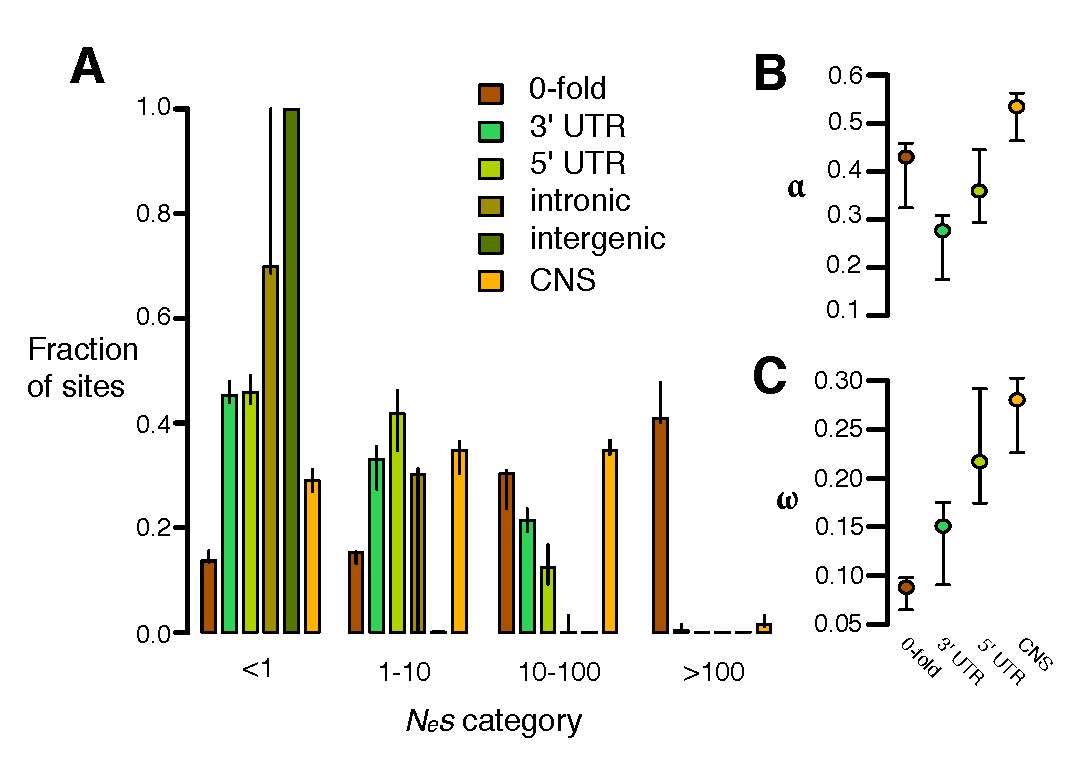
\includegraphics[scale=0.8]{Ch2Fig1}
    \caption{\textbf{Estimates of negative and positive selection on coding and noncoding sites in C. grandiflora.}A) The proportion of sites found in each bin of purifying selection strength, separated by site type, B) The proportion of divergent sites fixed by positive selection, and C) the rate of adaptive substitution relative to neutral divergence. Error bars represent 95\% bootstrap confidence intervals.}
    \label{fig:fig1}
\end{figure}

Genome-wide, we estimate that the proportion of intergenic sites that are nearly neutral approaches 100\% and that approximately 70\% of intronic sites are effectively neutral. Furthermore, bootstrapping results suggest that there is not significant support for less than 100\% of intronic sites being effectively neutral. The large confidence intervals around estimates of selection on intronic sites may be due to strong selection at splice site junctions [14] coupled with typically weak to no selection outside of splice junctions. To test for selection near splice junctions, we quantified selection acting on the first and last 30 bp of each intron separately from sites in the middle of introns. While 100\% of sites in the middle of introns are estimated to be effectively neutral, only 68\% of sites in junctions are, suggesting that our wide confidence intervals around intronic sites can be partially explained by variance caused by sampling sites in these different regions between bootstraps. These generally low estimates of Nes in (non-junction) intronic and intergenic sites imply a general lack of purifying selection in most noncoding regions, a lack of sensitivity to detect small proportions of selected sites, and/or nearly equivalent purifying selection to synonymous sites. 

Although our analysis suggests very low levels of purifying selection in noncoding regions other than UTRs and splice junctions, these global analyses may miss signatures of purifying selection on a small proportion of noncoding sites. One candidate set of sites that may have different signatures of selection are conserved noncoding sequences (CNSs); these are regions that show evidence of cross-species conservation, and are therefore prime candidates for functional noncoding sequences subject to selection. We identified CNSs across nine Brassicaceae genomes, following the implementation in Haudry et al. [14]. For this study, we used the Capsella genome as a reference for alignment, but excluded Capsella when identifying CNSs in order to avoid circularity when quantifying selection from diversity [8]. This method allows our analysis of selection on noncoding sites using polymorphism to be more independent of the comparative analysis. When we look at only these conserved regions in our C. grandiflora sample we see a small proportion of effectively neutral sites (28\%) compared to the noncoding regions as whole, suggesting that the majority of CNS sequences are subject to purifying selection (Fig.~\ref{fig:fig1}A). However, estimates suggest that CNSs are generally under weaker purifying selection than nonsynonymous (0-fold) sites and experience primarily weak and intermediate purifying selection (Fig.~\ref{fig:fig1}A). 

Although CNSs as a whole retain a considerable proportion of effectively neutral sites, it is of interest to examine whether particular classes of CNS show stronger selection. To examine differences between categories we quantified selection on the different types of CNSs separately (Fig.~\ref{fig:figS7}). In most categories, about 25\% of sites are nearly neutral, a slightly stronger signal of purifying selection than when we pool all CNSs. Intronic CNSs have a larger proportion of effectively neutral sites than other categories, in agreement with the general neutrality of intronic sites (Fig.~\ref{fig:fig1}). In contrast, small noncoding RNAs (sncCNSs) have a stronger signal of selection than the other CNS categories. However, the number of sites used to make the AFS for each of these categories varies substantially (Table S2), and our sample of sncCNSs has very little polymorphism (155 segregating sites). Nevertheless, despite the wide confidence intervals, sncCNSs still show a significantly (p < 0.001) smaller fraction of sites that are nearly neutral (Nes < 1) than the pooled CNSs, which could be due to strong selection for sequence specificity to obtain the proper secondary structure important for RNA activity [38]. This effect is consistent with sncCNSs showing a higher degree of conservation across the Brassicaceae [14] and having traceable orthologs in other plants.


\subsection{Genome-wide estimates of positive selection} 
We used the approach of Eyre-Walker and Keightley [28] to estimate the proportion of fixations driven by positive selection ($\alpha$) and the rate of positive selection ($\omega$) while taking into account the effect of slightly deleterious mutations, which can bias estimates of positive selection downwards. To do this, we estimated divergence using whole genome alignments of \textit{C. rubella}, \textit{A. thaliana}, and \textit{Neslia paniculata} (estimate of 4-fold synonymous divergence $K_{s}$ between \textit{C. rubella} and \textit{N. paniculata} is $K_{s}$=0.14). Because the large majority of noncoding sites are estimated to be effectively neutral, and because of alignment concerns between species in unconstrained noncoding regions, we focus our estimates of positive selection on 0-fold degenerate sites, CNS sites, and UTRs. We found that 0-fold degenerate sites show a very high proportion of divergence driven by positive selection  (Fig.~\ref{fig:fig1}B; $\alpha$ = 0.417) and estimates of the rate of adaptive substitution relative to synonymous substitution (Fig.~\ref{fig:fig1}C ; $\omega$ = 0.08). Similarly, UTRs and CNS sites show evidence for positive selection (Fig.~\ref{fig:fig1}B,C). These results generally suggest widespread positive selection in both nonsynonymous and functional noncoding genomic regions.

\begin{figure}[h!]
      \centering
       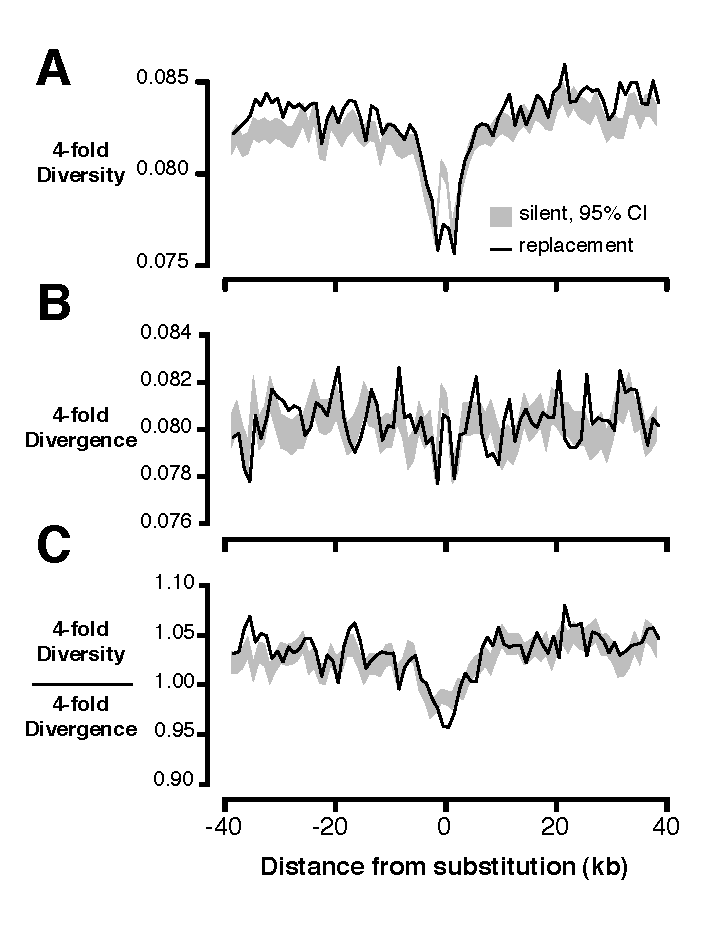
\includegraphics{Ch2Fig2}
    \caption{\textbf{Linked neutral diversity and divergence as a function of distance from fixed substitutions across the \textit{C. grandiflora genome}.} A) Diversity at 4-fold degenerate sites, B) Divergence at 4-fold degenerate sites, and C) Diversity/divergence at 4-fold degenerate sites. In all figures, black lines represent measures surrounding fixed replacement substitutions and gray shading represents 95\% confidence intervals, from bootstrapping, surrounding silent substitutions.).}
    \label{fig:fig2}
\end{figure}

If many of the amino acid changes between textit{C. grandiflora} and its nearest relatives are due to recent, strong positive selection from new mutations, we expect to see the signature of selective sweeps: reduced neutral diversity surrounding amino acid fixations [39,40]. We tested for this signature by measuring the proportion of 4-fold degenerate sites in each window that were polymorphic (referred to hereafter as '4-fold diversity') in non-overlapping 1kb windows surrounding fixed replacement (n = 60,378), and silent (n = 83,812) substitutions in \textit{C. grandiflora}. We found that 4-fold diversity surrounding fixed replacement substitutions was lower than 4-fold diversity surrounding fixed silent substitutions in the 4kb window surrounding substitutions (Fig.~\ref{fig:fig2}A). This result was robust to various window sizes from 500kb to 2kb (Fig.~\ref{fig:figS8}) and a one-tailed test for reduced 4-fold diversity around replacement sites was significant (p \textless  0.01 for 2 kb on either side of the substitution).

Patterns of diversity may be distorted by elevated mutation rates surrounding substitutions [39], which would increase diversity and divergence in \textit{C. grandiflora}. Consistent with this prediction, divergence at 4-fold degenerate sites ('4-fold divergence') is elevated around synonymous and replacement substitutions (Fig.~\ref{fig:fig2}B). To control for elevated mutation rate, we divided diversity by divergence at 4-fold degenerate sites (subsequently referred to as '4-fold diversity/divergence'). We observed a reduction in 4-fold diversity/divergence around replacement substitutions compared to silent substitutions, demonstrating that the signature of recurrent sweeps is not an artifact caused by variation in mutation rate (Fig.~\ref{fig:fig2}C, p \textless  0.01 for 1 kb on either side of the substitution).

\begin{figure}[h!]
      \centering
       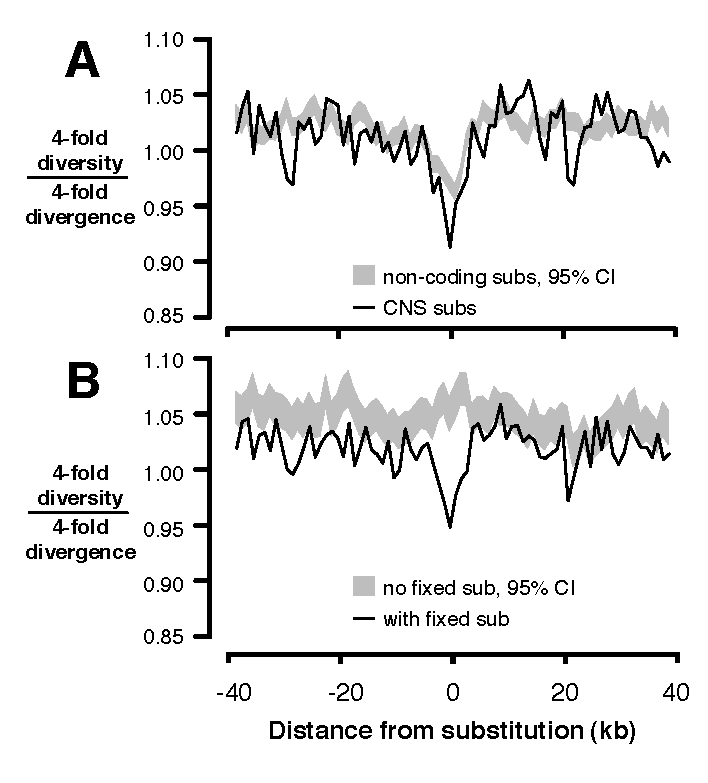
\includegraphics{Ch2Fig3}
    \caption{\textbf{Linked neutral diversity/divergence surrounding conserved noncoding sequences (CNSs).} Diversity/divergence at 4-fold degenerate sites as a function of distance from fixed substitutions in CNSs (black lines) and fixed substitutions in non-conserved intergenic sequence (gray shading, 95\% confidence interval).
B) Diversity/divergence at 4-fold degenerate sites as a function of distance from CNSs containing fixed substitutions (black line) and CNSs without any fixed substitutions (gray shading, 95\% confidence interval).}
    \label{fig:fig3}
\end{figure}

An analogous test for selective sweeps around fixations in noncoding regions is challenging because the test depends on accurately identifying interspersed functional and neutral sites, a difficult task in noncoding regions [8]. Instead, we compared 4-fold diversity and divergence around fixed substitutions in CNS regions (n = 12,578) with 4-fold diversity and divergence around fixed substitutions in non-conserved intergenic, intronic, and UTR regions (n = 117,178). Interestingly, there is a reduction in both 4-fold diversity and divergence surrounding fixed substitutions in CNSs compared to non-conserved noncoding regions (Fig.~\ref{fig:figS9}). It is not clear why 4-fold divergence decreases around CNS substitutions; it is possible that in genomic scans for conserved regions, large-scale constraint might span both coding and noncoding sequence, causing non-independence and reducing divergence at 4-fold degenerate sites near CNSs. However, there is still a reduction in 4-fold diversity/divergence around fixed substitutions in CNSs compared to those in non-conserved intergenic regions, consistent with the action of recurrent selective sweeps (Fig.~\ref{fig:fig3}A). 

The observed reduction in diversity/divergence around CNS substitutions could also reflect the action of background purifying selection; sites closer to CNSs may experience a reduction of neutral diversity due to greater purifying selection on mutations in CNSs. This effect is not a problem for comparisons between replacement and silent substitutions because they are interspersed within the same exons, so diversity and divergence around these sites experience the same background selection. To ensure that the reduction in diversity/divergence surrounding CNS substitutions compared to non-conserved noncoding substitutions is not due to differences in background selection between CNS and intergenic sites, we compared neutral diversity and divergence surrounding CNSs that contain at least one fixed substitution to neutral diversity and divergence around those that do not. There is a reduction in neutral diversity/divergence surrounding CNSs containing a fixed substitution (n = 12,884) compared to CNSs without fixed substitutions (n = 41,212), suggesting that this signature of recurrent sweeps is not driven by background selection specific to CNSs (Fig.~\ref{fig:fig3}B).

\subsection{Effects of expression and selection}
We measured expression levels of all expressed genes using RNA extracted from leaf tissue of 10 of the 13 \textit{C. grandiflora} individuals. Genes were sorted by mean expression level and split into four equally sized groups, which will be referred to as “high”, “mid-high”, “mid-low”, and “low” expression genes. We calculated polymorphism within \textit{C. grandiflora} and lineage-specific divergence from \textit{N. paniculata} and \textit{A. thaliana} for sites within these genes. As expected from previous studies, $d_{N}/d_{S}$ is considerably lower in high expression genes (0.15) than low expression genes (0.22).  In addition, $d_{N}/d_{S}$ is negatively correlated with expression level across all genes (correlation coefficient = -0.051, p \textless 0.001).

To test whether the strength of negative selection differs between expression categories we compared the allele frequency spectra of sites in different expression categories. Replacement polymorphisms in high expression genes show a stronger skew towards rare alleles than those in low expression genes (FIg.~\ref{fig:figS10}). In addition, a larger proportion of replacement sites are invariant in high expression genes (98.9\%), than in low expression genes (97.8\%), consistent with stronger negative selection. Comparisons of the distribution of fitness effects show that high expression genes have a much smaller proportion of effectively neutral sites (6.8\%) than low expression genes (16\%, randomization test [28], p \textless  0.001) (Fig.~\ref{fig:fig4}A).  

\begin{figure}[h]
      \centering
       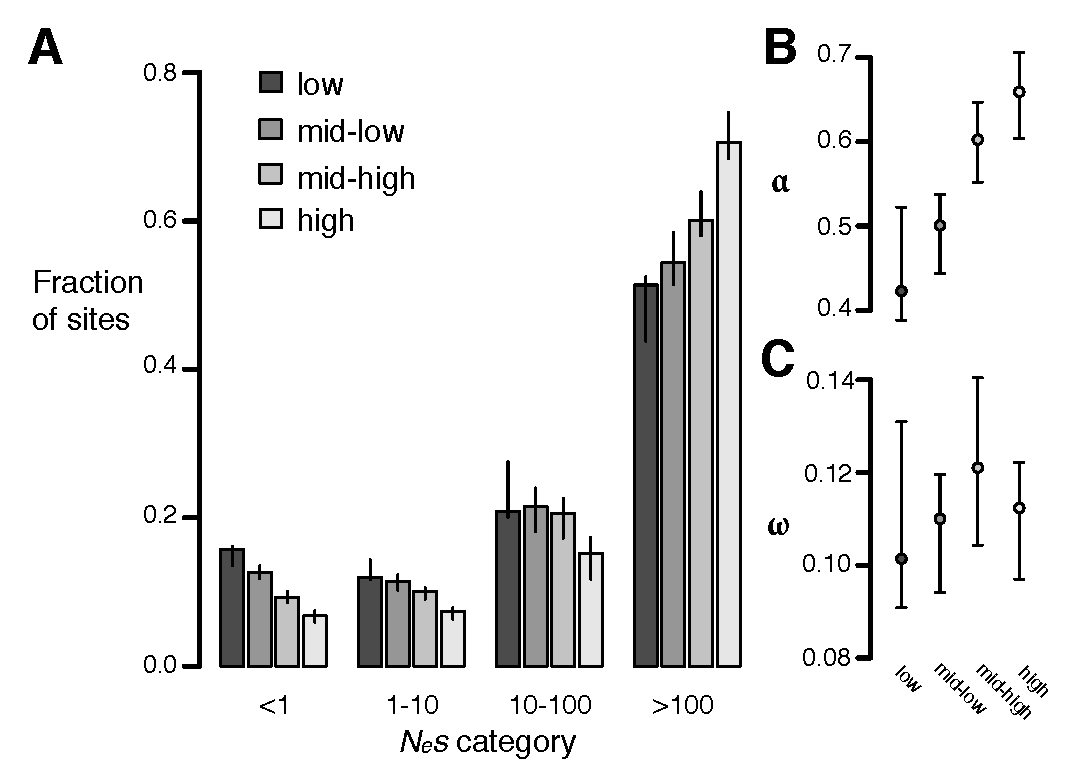
\includegraphics[scale=0.8]{Ch2Fig4}
    \caption{\textbf{Estimates of negative and positive selection on nonsynonymous sites in genes of varying expression level.}A) The proportion of sites found in each bin of purifying selection strength, separated by expression level.  B) The proportion of divergent sites fixed by positive selection and C) The rate of adaptive substitution relative to neutral divergence. Error bars represent 95\% bootstrap confidence intervals. }
    \label{fig:fig4}
\end{figure}

Increased divergence in low expression genes relative to high expression genes could also be caused by increased positive selection in low expressed genes compared to highly expressed genes. To test this possibility, we calculated $\alpha$ and $\omega$ as described above. High expression genes have a significantly higher value of $\alpha$ (0.66) than low expression genes (0.42, p \textless 0.01) but the $\omega$ value for both classes is similar (high: 0.11, low: 0.10, p = 0.38), suggesting that the rate of positive selection does not differ between high and low expression genes (Fig.~\ref{fig:fig4}B,C). The difference in $\alpha$ between the two categories likely reflects the reduction in the number of weakly deleterious and effectively neutral mutations that are able to fix due to stronger purifying selection in high expression genes compared to low expression genes, causing a higher proportion of those amino acids that do reach fixation to be positively selected. 


\section{Discussion}
In this population genomic survey of \textit{C. grandiflora}, we demonstrated that positive and negative selection contribute to DNA sequence variation in protein-coding regions, UTRs, and CNSs. We also showed that differences in divergence between high and low expression genes are due to increased negative selection in high expression genes, not increased positive selection in low expression genes. In addition, we found a clear signature of recurrent selective sweeps contributing to divergence in coding regions as well as CNSs. Overall, our evidence for widespread positive and negative selection in \textit{C. grandiflora} is in line with expectations, given its outcrossing mating system, large $N_{e}$, limited population structure, and lack of a recent whole genome duplication [6].

In contrast, selection appears to be very rare in intergenic and (non-junction) intronic regions that are not conserved across Brassicaceae species. In particular, we cannot detect significant evidence of purifying selection in intergenic or intronic regions as a whole, suggesting that selected sites within these regions must be rare or absent. However, when we only examine CNSs, we do see evidence of selection, indicating that at least 5\% of sites in intergenic regions are selected, but the DFE approach is not sensitive enough to detect selection on such a small subset of intergenic sites. This result implies that this approach is likely to also be missing lineage-specific selection when it comprises a relatively small fraction of sites, and it highlights the importance of integrating additional evidence of function (comparative and experimental) for improved quantification of selection.
The general neutrality of noncoding regions, based on population genomic analysis, is consistent with the conclusions of Haudry and colleagues [14], who used comparative genomics approaches to estimate that only 5\% of noncoding bases are under selection in the Arabidopsis genome. This result contrasts with Drosophila and humans, where a relatively large fraction of selected sites are found in noncoding regions [6]. For example, in Drosophila, only 30\%-70\% of intronic and intergenic regions are nearly neutral [2,28,29]. Similarly, Halligan et. al. [8] recently used information from the DFE to infer the number of adaptive substitutions in mice both in coding and noncoding regions. They show that the majority (approximately 80\%) of the adaptive substitutions in the mouse genome are in noncoding regions and suggest that they may have regulatory function. In contrast, our data show that C. grandiflora has similar numbers of adaptive substitutions in 0-fold sites (50.6 kb) and noncoding sites (21.6 kb, 3’ UTR excluding CNSs; 10.2 kb, 5’ UTR excluding CNSs; 32.7 kb, CNS; 64.4 kb total). Additionally, the width of diversity reductions surrounding replacement substitutions and substitutions in CNS regions appear comparable, suggesting that there is little evidence for a difference in the strength of positive selection on substitutions in coding regions compared to conserved noncoding regions. Our results are consistent with previous suggestions that, unlike in animals, plant genomes may contain fewer noncoding regulatory sequences subject to positive and negative selection, possibly because gene expression can be modified through frequent gene duplication and functional divergence rather than through the evolution of novel regulatory elements [13]. In future work, it would be interesting to quantify the extent to which adaptive changes in gene expression in plants occur following gene duplication relative to between-species divergence at orthologous genes.

Unlike other classes of noncoding sequence, UTRs show relatively high levels of purifying selection, likely reflective of their function in post-transcriptional regulation [41]. UTRs are also under stronger negative selection than other noncoding regions in Drosophila [2], and this result is also in line with the previous study using comparative genomics in the Brassicaceae [14]. Interestingly, we infer that a large fraction of selected sites in UTRs may be outside of CNS regions identified in between-species comparisons. In particular, using estimates of the proportion of sites under selection, we estimate that 88\% of 3’ UTR and 77\% of 5’ UTR selected sites are outside of conserved regions.  This result suggests that there may be many species-specific (i.e., non-CNS) functional regions in UTRs and they may therefore play an important role in recent or local adaptation.

One important consideration is the extent to which our analyses are truly reflective of genome-wide patterns of selection. Despite whole genome sequencing, our analyses are restricted to approximately 20\% of the genome, and only 10\% of intergenic sites, largely due to the fact that a large fraction of the genome is pericentromeric, repetitive and/or surrounds insertion/deletion events. It is important to recognize that our estimates of selection apply strictly to this ‘accessible’ genome and that the extent of purifying and positive selection on the repetitive regions remains difficult to assess. Nevertheless, we would expect that our conclusions about low levels of purifying and positive selection across most noncoding regions are likely conservative with respect to these filters because a large proportion of repetitive DNA is likely to be neutral. On the other hand, rates of positive selection may be elevated in coding regions of duplicate genes filtered out of our analysis [42], suggesting that our estimates of positive selection in protein-coding regions may also be a lower bound.   
A second concern is the extent to which synonymous sites are neutrally evolving. Although analysis of codon usage bias from population genetic data does suggest the action of some purifying selection on synonymous sites in this species [43], the strength of selection inferred is close to effective neutrality. Furthermore, synonymous site selection is expected to be stronger in more high expression genes [23,44], causing us to underestimate, rather than overestimate, the difference in the strength of purifying selection compared with low expression genes. Thus, while selection on synonymous sites may bias our estimates of selection slightly downward, our general conclusions are likely to be robust to violations of neutrality. Nevertheless, more investigation of the action of selection on synonymous sites is important, particularly given growing evidence for synonymous site selection that may reflect gene regulation, in addition to codon usage [45,46].

At synonymous sites, we see an excess of rare variants, as indicated by a negative Tajima’s D. The excess of rare variants is unlikely to be explained by a high Illumina error rate, as our observed value of -0.51 is nearly identical to a previous estimate (-0.52) from Sanger-sequenced loci and a comparable geographic sampling [27]. This previous study found that, while population subdivision was low compared to other herbaceous species studied, there were still three major geographic clusters (average between-population Fst of 0.11). If we restrict our dataset to one of the three geographic regions based on these previous results, Tajima’s D approaches zero (-0.16 at 4-fold degenerate sites), suggesting that the excess of rare variants at synonymous sites may be largely due to population structure. 

\subsection{Measuring positive selection}
	In this study, we took advantage of the two detectable signatures expected to remain after recurrent classic selective sweeps from new mutations: 1) an excess of replacement substitutions relative to expectations based on polymorphism, and 2) reduced neutral diversity near fixed differences. Our findings strongly suggest that positive selection has been common in coding regions, UTRs and conserved noncoding regions in \textit{C. grandiflora} and that classic selective sweeps contribute significantly to divergence in these regions. To our knowledge, this is the first time that the signature of recurrent selective sweeps has been observed in a non-Drosophila species, despite being tested in other species [8,47]. Our ability to detect the signature of recurrent sweeps may be because \textit{C. grandiflora} has relatively low linkage disequilibrium, increasing power.

However, many positively selected alleles may not follow the trajectory of a classic selective sweep. Soft sweeps — adaptation from an allele previously maintained in the population by mutation-selection-drift balance or the simultaneous fixation of multiple independently derived mutations at the same allele — may still increase the replacement to silent divergence ratio, but are expected to have a smaller effect on linked neutral diversity [48-50]. We expect that soft sweeps will also be common in \textit{C. grandiflora} because of its large Ne [50,51]. In addition, adaptation in genes that contribute to polygenic traits is often expected to occur without fixation of new mutations [52], and this will be missed by both of our tests for positive selection. These considerations suggest that both measures of positive selection are conservative and may miss many instances of positive selection acting in the genome.
Our conclusions about the prevalence of selective sweeps in \textit{C. grandiflora} may seem to conflict with our observation that diversity and Tajima's D are slightly higher at 4-fold degenerate sites than intergenic sites, since frequent sweeps in coding regions should reduce diversity more strongly in sites near and within genes. There are two likely contributors to this discrepancy. First, recurrent sweeps may in fact reduce average diversity in 4-fold degenerate sites and, by using these sites to set neutral expectations, we are underestimating the strength of purifying selection in intergenic regions. Second, because recombination rates are relatively high, and intergenic regions near coding regions relatively small in Capsella, the average impact of linked selection may be similar at 4-fold degenerate sites and intergenic sequences. 

\subsection{Expression level and selection}
	Highly expressed genes diverge less than genes with low expression in many species [15-17,19,24,53-55]. This pattern could be due to stronger positive selection in low expression genes or stronger negative selection in high expression genes, or both. Our results suggest that variation in divergence rates between high and low expression genes is largely due to increased negative selection in high expression genes compared to low expression genes. This result is consistent with previous studies that have suggested that new nonsynonymous mutations that cause protein mis-folding or mis-interaction will have stronger deleterious effects in high expression genes than low expression genes and that new mutations that cause mRNA mis-folding are under stronger negative selection in high expression genes than low expression genes [23-25]. In addition, our results agree with a similar study in Medicago truncatula that found stronger purifying selection in genes that were expressed than in genes that were not expressed [20]. 


\section{Methods}
\subsection{Sampling and sequencing}
Population samples for \textit{C. grandiflora} represented a ‘scattered’ sample of one individual per population for twelve populations from across the geographic range in Greece, plus a thirteenth sample that was the product of a cross of two additional populations (Table S1). Plants were grown for several months at the University of Toronto greenhouse, and genomic DNA was extracted from leaf tissue using a modified CTAB protocol. Library preparation and single-end genomic sequencing were conducted at the Genome Quebec Innovation Centre at McGill University on the Illumina GAII platform. Each sample was sequenced in 2 to 3 lanes and with a read length of 108 bp.

Leaves from 10 of the 13 individuals were collected and flash frozen for RNA extraction using Qiagen's RNAeasy plant extraction kit. This RNA was sequenced at the Genome Quebec Innovation Centre, on an Illumina GAII platform with one individual per lane, generating single-end 108 bp long reads. The RNA sequence from these 10 individuals was used for the annotation of the \textit{C. rubella} reference genome, as reported in [30], but the raw sequence data was reanalyzed for this study (see below).

\subsection{Genotyping}
Genomic reads were aligned to the \textit{C. rubella} reference genome [30] using the Stampy aligner 1.0.13 with default settings [56]. Sites around indels were realigned using the Genome Analysis Toolkit (GATK) v1.05777 indel realigner [31]. Genotype and SNP calls were conducted using the GATK UnifiedGenotyper with default parameters [57], after aligning and genotyping the median site quality was 89 and the median individual depth across all sites was 34. 

To get a rough assessment of genotyping error rates, we conducted Sanger sequencing from nine coding regions in six of our individuals. From a total of 16,389 bp of Sanger sequence, we found 8 differences between Sanger and Illumina genotypes, giving an estimated error rate of 0.00049. Three of these disagreements were due to three segregating bases at a single site, which we excluded in our GATK genotyping protocol. As we suspect several of these disagreements may be due to Sanger sequencing errors due to variation in allelic representation of heterozygotes, this provides an upper bound estimate of error rate in coding regions, although higher indel rates and repetitive sequence in noncoding DNA may lead to a higher error rate in those regions. 

AFSs were generated from counts of sites in the VCF. Invariant sites were excluded from the AFS if (1) the site quality score was below 90, (2) the fraction of reads containing spanning deletions was not 0 (i.e. the 'Dels' value was greater than zero), or (3) any individual's read depth was less than 20 or greater than 60. Additionally, polymorphic sites were excluded, based on filters 1-3, if (4) the most likely genotype of any individual did not have a phred scaled likelihood score of 0, and if (5) the second most likely genotype had a phred likelihood score less than 40. Additionally, entire regions of the genome were filtered out of the analysis if less than 30\% of the sites in a 20kb window passed all other filters. This final filter primarily eliminated pericentromeric regions that were highly repetitive, where we were not confident in genotype calls and observed high heterozygosity.

Our data showed evidence of identity by descent (IBD) in some samples (Fig. ~\ref{fig:figS4}). We identified these regions by splitting the genome into 200kb windows, then calculating FIS (Fig. ~\ref{fig:figS4}). If FIS was greater than 0.5, the region was flagged as IBD. Across all samples no more than 3 of these regions overlapped. For further analyses we downsampled data in other regions down to 23 chromosomes treating any region of IBD as haploid to ensure that no IBD region was sampled twice from the same individual.

\subsection{Divergence}

We calculated lineage-specific divergence in two ways. First, we aligned the \textit{C. rubella} reference sequence with sequence data from \textit{A. thaliana} and \textit{N. paniculata} using lastZ [58] with chaining, as previously described [14]. In order to get an estimate of divergence unique to the Capsella lineage, we called sites as diverged where \textit{A. thaliana} and \textit{N. paniculata} had the same nucleotide and this nucleotide differed in the \textit{C. rubella} sequence. If any of the three species was missing data at a site, then that site, and sites 5 bp upstream and downstream of the site, were excluded from divergence analyses in order to avoid inflating divergence because of spurious alignments around indels.

We used a second method for calculating divergence for comparisons that included only coding sequences, particularly for the comparison of genes with different expression levels. We found orthologs between \textit{C. rubella}, \textit{A. thaliana} and \textit{N. paniculata} genes using InParanoid [59] and MultiParanoid [60]. The peptide sequences of these orthologs were aligned using DialignTX [61], and reverse-translated into coding sequence. Whole-gene divergence at synonymous and nonsynonymous sites was calculated, using PAML [62], under a model where $\omega$ was allowed to vary in the Capsella lineage compared to other branches.

We conducted comparisons of estimates of the distribution of fitness effects using the two methods above with identical gene sets, and found a very strong concordance of results (see Fig.~\ref{fig:fig4} compared to Fig.~\ref{fig:figS11}). Furthermore, while we don't predict a significant effect on results, it is important to note that the two methods also differed in how selected and nonselected classes were determined: the first distinguishes between 0-fold and 4-fold sites and discards other sites, while the second distinguishes between synonymous and nonsynonymous sites, including all data. However, both approaches gave comparable estimates of positive and negative selection.

\subsection{Identifying conserved noncoding sequences}
Conserved noncoding sequences (CNS) were identified in the \textit{C. rubella} genome by first obtaining whole-genome multiple alignments, using a variant of the lastZ/Multiz pipeline previously described [14,63] and using \textit{C. rubella} as the reference genome. The \textit{C. rubella} genome sequence was then neutralized (bases replaced with N) and the PhastCons tool used to quantify family-wide levels of conservation. CNSs were then identified, based on extended (>12nt) near-continuous regions of high conservation as previously described [14].   

\subsection{Estimates of the distribution of fitness effects and $\alpha$}
Site categories were determined based on the Joint Genome Institute’s gene annotation of the \textit{C. rubella} reference genome [30]. The allele frequency spectra (AFS) and divergence values were calculated for each category of sites, and DFE-alpha [28,64] was used to estimate the fraction of sites under negative selection and α, using 4-fold degenerate sites as the neutral reference. The genome was broken up into 10 kb regions and these regions were bootstrapped 200 times to generate 95\% CIs for selection on each category of sites. We tested for a significant difference in selection between the pooled set of CNSs and each individual category of CNSs using a randomization test, as in Keightley and Eyre-Walker [28], by calculating the proportion of bootstraps where selection was higher in the pooled set of CNS versus the category of interest. Because this is a two-tailed test, we report twice this proportion as the p value. 

\subsection{Test for signatures of recurrent selective sweeps}
We used the multiple species alignments of orthologous genes, generated as described above, to identify silent and replacement single-nucleotide sites that were the same in A. thaliana and N. paniculata but differed in the \textit{C. rubella} reference, suggesting that the substitution had most likely occurred in the Capsella lineage after divergence from \textit{N. paniculata}. From these substitutions, we identified those that did not diverge between \textit{C. rubella} and \textit{C. grandiflora} and were fixed in \textit{C. grandiflora}.

We calculated neutral diversity in sliding windows around fixed substitutions by calculating the proportion of 4-fold degenerate sites within these windows that were polymorphic in \textit{C. grandiflora} (i.e., the proportion of segregating sites). Neutral divergence was measured by calculating the proportion of 4-fold sites within these windows that diverged in the Capsella lineage. Diversity/divergence was calculated by dividing diversity by divergence in each window. We conducted this analysis for windows of 500bp, 1kb, and 2kb, extending 40kb from each substitution. We chose this window size range to match analysis done in Sattath et al [39]. For each of the above measures, we bootstrapped by substitution (n=1000) and removed the top and bottom 25 bootstraps to construct 95\% confidence intervals. Following Hernandez and colleagues [47], we tested the null hypothesis that diversity/divergence around replacement and silent substitutions does not differ by calculating a one-tailed p value for each window, equal to (i+1)/(n+2) where i is the number of bootstraps in which diversity/divergence around silent sites is lower or equal to the actual diversity/divergence around replacement sites, and n is the total number of bootstraps.

To detect the effects of linked selection on noncoding DNA, we compared diversity around fixed substitutions within CNSs to diversity around fixed substitutions in non-conserved intergenic regions. To find these substitutions, we compared the multiple sequence alignments of the CNSs between \textit{C. grandiflora}, \textit{N. paniculata}, and \textit{A. thaliana} and chose sites that differed between \textit{C. grandiflora} and the other species and were fixed within \textit{C. grandiflora}. Additionally, we compared neutral diversity around CNSs with at least one fixed substitution to neutral diversity around CNSs without any fixed substitutions. 

\subsection{Gene expression}
	Illumina sequencing generated 331,629,531 reads for 10 individuals, ranging from 31,267,774 to 35,552,133 reads per individual. This RNA sequence was mapped to the \textit{C. rubella} reference genome using Tophat 1.2.0 [65], and expression level was quantified from these mapped reads using Cufflinks 1.3.0 [66]. Cufflinks standardizes expression levels by gene length and library size, returning values in units of 'fragments per kilobase of exon per million fragments mapped' (FPKM). We calculated the mean expression level for each gene across our 10 samples and removed those genes with <1 FKPM to eliminate genes that may have been mis-annotated. The remaining 11,564 genes were divided into four, roughly equally sized categories based on expression level: low (1-6.8 FPKM), mid-low (6.8 – 17.5 FPKM), mid-high (17.5-44.7 FPKM), and high (44.7 – 17,092 FPKM). The distribution of fitness effects, α, and ω were calculated for each gene set, using the same protocol described above. We bootstrapped each gene set by sampling genes with replacement 1000 times to generate 95\% confidence intervals for selection strength. Using the same methods described for tests of differences within the CNSs categories above, we tested for a significant difference in selection strength between high and low expression genes.

\section{Acknowledgements}
We thank Peter Keightley and Dan Halligan for advice and custom scripts, Yunchen Gongß and Emilio Vello for technical assistance, Tanja Slotte, Kate St. Onge, and John Paul Foxe for collecting seeds, and Detlef Weigel, Dan Koenig, Thomas Bureau, Alan Moses, Daniel Schoen, and John Stinchcombe for helpful discussion and/or comments on the manuscript. We would also like to thank Jeff Ross-Ibarra and two anonymous reviewers for helpful comments on the manuscript.

\section{References}


1.	Keightley PD, Eyre-Walker A (2010) What can we learn about the distribution of fitness effects of new mutations from DNA sequence data? Philos Trans R Soc Lond B Biol Sci 365: 1187–1193. doi:10.1098/rstb.2009.0266.

2.	Andolfatto P (2005) Adaptive evolution of non-coding DNA in Drosophila. Nature 437: 1149–1152. doi:10.1038/nature04107.

3.	Torgerson DG, Boyko AR, Hernandez RD, Indap A, Hu X, et al. (2009) Evolutionary processes acting on candidate cis-regulatory regions in humans inferred from patterns of polymorphism and divergence. PLoS Genet 5: e1000592. doi:10.1371/journal.pgen.1000592.

4.	Lindblad-Toh K, Garber M, Zuk O, Lin MF, Parker BJ, et al. (2011) A high-resolution map of human evolutionary constraint using 29 mammals. Nature 478: 476–482. doi:10.1038/nature10530.

5.	Arbiza L, Gronau I, Aksoy BA, Hubisz MJ, Gulko B, et al. (2013) Genome-wide inference of natural selection on human transcription factor binding sites. Nat Genet 45: 723–729. doi:10.1038/ng.2658.

6.	Hough J, Williamson RJ, Wright SI (2013) Patterns of selection in plant genomes. Annu Rev Ecol Evol Syst 44: 3.1–3.19. doi:10.1146/annurev-ecolsys-110512-135851.

7.	Zhen Y, Andolfatto P (2012) Methods to detect selection on noncoding DNA. Methods in Molecular Biology. Totowa, NJ: Humana Press, Vol. 856. pp. 141–159. doi:10.1007/978-1-61779-585-5\_6.

8.	Halligan DL, Kousathanas A, Ness RW, Harr B, Eőry L, et al. (2013) Contributions of protein-coding and regulatory change to adaptive molecular evolution in murid rodents. PLoS Genet 9: e1003995. doi:10.1371/journal.pgen.1003995.

9.	Wray GA (2007) The evolutionary significance of cis-regulatory mutations. Nat Rev Genet 8: 206–216. doi:10.1038/nrg2063.

10.	Carroll SB (2005) Evolution at two levels: on genes and form. PLoS Biol 3: e245. doi:10.1371/journal.pbio.0030245.

11.	Hoekstra HE, Coyne JA (2007) The locus of evolution: evo devo and the genetics of adaptation. Evolution 61: 995–1016. doi:10.1111/j.1558-5646.2007.00105.x.

12.	Keightley PD, Gaffney DJ (2003) Functional constraints and frequency of deleterious mutations in noncoding DNA of rodents. Proc Natl Acad Sci USA 100: 13402–13406. doi:10.1073/pnas.2233252100.

13.	Lockton S, Gaut BS (2005) Plant conserved non-coding sequences and paralogue evolution. Trends Genet 21: 60–65. doi:10.1016/j.tig.2004.11.013.

14.	Haudry A, Platts AE, Vello E, Hoen DR, Leclercq M et al. (2013) An atlas of over 90,000 conserved noncoding sequences provides insight into crucifer regulatory regions. Nat Genet. doi:doi:10.1038/ng.2684.

15.	Pál C, Papp B, Hurst LD (2001) Highly expressed genes in yeast evolve slowly. Genetics 158: 927–931.

16.	Subramanian S, Kumar S (2004) Gene expression intensity shapes evolutionary rates of the proteins encoded by the vertebrate genome. Genetics 168: 373–381. doi:10.1534/genetics.104.028944.

17.	Drummond DA, Raval A, Wilke CO (2006) A single determinant dominates the rate of yeast protein evolution. Mol Biol Evol 23: 327–337. doi:10.1093/molbev/msj038.

18.	Yang L, Gaut BS (2011) Factors that contribute to variation in evolutionary rate among Arabidopsis genes. Mol Biol Evol 28: 2359–2369. doi:10.1093/molbev/msr058.

19.	Slotte T, Bataillon T, Hansen TT, St Onge K, Wright SI, et al. (2011) Genomic determinants of protein evolution and polymorphism in Arabidopsis. Genome Biol Evol 3: 1210–1219. doi:10.1093/gbe/evr094.

20.	Paape T, Bataillon T, Zhou P, J Y Kono T, Briskine R, et al. (2013) Selection, genome-wide fitness effects and evolutionary r
ates in the model legume Medicago truncatula. Mol Ecol 22: 3525–3538. doi:10.1111/mec.12329.
21.	Renaut S, Grassa CJ, Moyers BT, Kane NC, Rieseberg LH (2012) The population genomics of sunflowers and genomic determinants of protein evolution revealed by RNAseq. Biology (Basel) 1: 575–596. doi:10.3390/biology1030575.

22.	Gaut B, Yang L, Takuno S, Eguiarte LE (2011) The patterns and causes of variation in plant nucleotide substitution rates. Annu Rev Ecol Evol Syst 42: 245–266. doi:10.1146/annurev-ecolsys-102710-145119.

23.	Park C, Chen X, Yang J-R, Zhang J (2013) Differential requirements for mRNA folding partially explain why highly expressed proteins evolve slowly. Proc Natl Acad Sci USA 110: E678–E686. doi:10.1073/pnas.1218066110.

24.	Yang J-R, Liao B-Y, Zhuang S-M, Zhang J (2012) Protein misinteraction avoidance causes highly expressed proteins to evolve slowly. Proc Natl Acad Sci USA 109: E831–E840. doi:10.1073/pnas.1117408109.

25.	Drummond DA, Wilke CO (2008) Mistranslation-induced protein misfolding as a dominant constraint on coding-sequence evolution. Cell 134: 341–352. doi:10.1016/j.cell.2008.05.042.
26.	Gossmann TI, Song B-H, Windsor AJ, Mitchell-Olds T, Dixon CJ, et al. (2010) Genome wide analyses reveal little evidence for adaptive evolution in many plant species. Mol Biol Evol 27: 1822–1832. 

27.	St Onge KR, Källman T, Slotte T, Lascoux M, Palmé AE (2011) Contrasting demographic history and population structure in Capsella rubella and Capsella grandiflora, two closely related species with different mating systems. Mol Ecol 20: 3306–3320. doi:10.1111/j.1365-294X.2011.05189.x.

28.	Eyre-Walker A, Keightley PD (2009) Estimating the rate of adaptive molecular evolution in the presence of slightly deleterious mutations and population size change. Mol Biol Evol 26: 2097–2108. doi:10.1093/molbev/msp119.

29.	Sella G, Petrov DA, Przeworski M, Andolfatto P (2009) Pervasive natural selection in the Drosophila genome? PLoS Genet 5: e1000495. doi:10.1371/journal.pgen.1000495.

30.	Slotte T, Hazzouri KM, Agren JA, Koenig D, Maumus F, et al. (2013) The Capsella rubella genome and the genomic consequences of rapid mating system evolution. Nat Genet 45: 831–835. doi:10.1038/ng.2669.

31.	McKenna A, Hanna M, Banks E, Sivachenko A, Cibulskis K, et al. (2010) The Genome Analysis Toolkit: a MapReduce framework for analyzing next-generation DNA sequencing data. Genome Res 20: 1297–1303. doi:10.1101/gr.107524.110.

32.	Slotte T, Foxe JP, Hazzouri KM, Wright SI (2010) Genome-wide evidence for efficient positive and purifying selection in Capsella grandiflora, a plant species with a large effective population size. Mol Biol Evol 27: 1813–1821. 

33.	Clark RM, Schweikert G, Toomajian C, Ossowski S, Zeller G, et al. (2007) Common sequence polymorphisms shaping genetic diversity in Arabidopsis thaliana. Science 317: 338–342. doi:10.1126/science.1138632.

34.	Wright SI, Foxe JP, DeRose-Wilson L, Kawabe A, Looseley M, et al. (2006) Testing for effects of recombination rate on nucleotide diversity in natural populations of Arabidopsis lyrata. Genetics 174: 1421–1430. doi:10.1534/genetics.106.062588.

35.	Kawabe A, Forrest A, Wright SI, Charlesworth D (2008) High DNA sequence diversity in pericentromeric genes of the plant Arabidopsis lyrata. Genetics 179: 985–995. doi:10.1534/genetics.107.085282.

36.	Branca A, Paape TD, Zhou P, Briskine R, Farmer AD, et al. (2011) Whole-genome nucleotide diversity, recombination, and linkage disequilibrium in the model legume Medicago truncatula. Proc Natl Acad Sci USA 108: E864–E870. doi:10.1073/pnas.1104032108.

37.	Slotte T (2014) The impact of linked selection on plant genomic variation. Brief Funct Genomics. doi:10.1093/bfgp/elu009.

38.	Ehrenreich IM, Purugganan MD (2008) Sequence variation of MicroRNAs and their binding sites in Arabidopsis. Plant Physiol 146: 1974–1982. doi:10.1104/pp.108.116582.

39.	Sattath S, Elyashiv E, Kolodny O, Rinott Y, Sella G (2011) Pervasive adaptive protein evolution and diversity patterns around amino acid substitutions in Drosophila simulans. PLoS Genet 7: e1001302. 

40.	Smith JM, Haigh J (1974) The hitch-hiking effect of a favourable gene. Genet Res 23: 23–35. doi:10.1017/S0016672308009579.

41.	Kim Y, Lee G, Jeon E, Sohn EJ, Lee Y, et al. (2013) The immediate upstream region of the 5'-UTR from the AUG start codon has a pronounced effect on the translational efficiency in Arabidopsis thaliana. Nucleic Acids Res. doi:10.1093/nar/gkt864.

42.	Han MV, Demuth JP, McGrath CL, Casola C, Hahn MW (2009) Adaptive evolution of young gene duplicates in mammals. Genome Res 19: 859–867. doi:10.1101/gr.085951.108.

43.	Qiu S, Zeng K, Slotte T, Wright S, Charlesworth D (2011) Reduced efficacy of natural selection on codon usage bias in selfing Arabidopsis and Capsella species. Genome Biol Evol 3: 868–880. doi:10.1093/gbe/evr085.

44.	Wright SI, Yau CBK, Looseley M, Meyers BC (2004) Effects of gene expression on molecular evolution in Arabidopsis thaliana and Arabidopsis lyrata. Mol Biol Evol 21: 1719–1726. doi:10.1093/molbev/msh191.

45.	Duret L, Mouchiroud D (1999) Expression pattern and, surprisingly, gene length shape codon usage in Caenorhabditis, Drosophila, and Arabidopsis. Proc Natl Acad Sci USA 96: 4482–4487.

46.	Marais G, Mouchiroud D, Duret L (2001) Does recombination improve selection on codon usage? Lessons from nematode and fly complete genomes. Proc Natl Acad Sci USA 98: 5688–5692.

47.	Hernandez RD, Kelley JL, Elyashiv E, Melton SC, Auton A, et al. (2011) Classic selective sweeps were rare in recent human evolution. Science 331: 920–924. doi:10.1126/science.1198878.

48.	Pennings PS, Hermisson J (2006) Soft sweeps II--molecular population genetics of adaptation from recurrent mutation or migration. Mol Biol Evol 23: 1076–1084. doi:10.1093/molbev/msj117.

49.	Pennings PS, Hermisson J (2006) Soft sweeps III: the signature of positive selection from recurrent mutation. PLoS Genet 2: e186. doi:10.1371/journal.pgen.0020186.

50.	Hermisson J, Pennings PS (2005) Soft sweeps: molecular population genetics of adaptation from standing genetic variation. Genetics 169: 2335–2352. doi:10.1534/genetics.104.036947.

51.	Messer PW, Petrov DA (2013) Population genomics of rapid adaptation by soft selective sweeps. Trends Ecol Evol 28: 659–669. doi:10.1016/j.tree.2013.08.003.

52.	Pavlidis P, Metzler D, Stephan W (2012) Selective sweeps in multilocus models of quantitative traits. Genetics 192: 225–239. doi:10.1534/genetics.112.142547.

53.	Lemos B, Bettencourt BR, Meiklejohn CD, Hartl DL (2005) Evolution of proteins and gene expression levels are coupled in Drosophila and are independently associated with mRNA abundance, protein length, and number of protein-protein interactions. Mol Biol Evol 22: 1345–1354. doi:10.1093/molbev/msi122.

54.	Drosophila 12 Genomes Consortium, Clark AG, Eisen MB, Smith DR, Bergman CM, et al. (2007) Evolution of genes and genomes on the Drosophila phylogeny. Nature 450: 203–218. doi:10.1038/nature06341.

55.	Carneiro M, Albert FW, Melo-Ferreira J, Galtier N, Gayral P, et al. (2012) Evidence for widespread positive and purifying selection across the European rabbit (Oryctolagus cuniculus) Genome. Mol Biol Evol 29: 1837–1849. doi:10.1093/molbev/mss025.

56.	Lunter G, Goodson M (2011) Stampy: a statistical algorithm for sensitive and fast mapping of Illumina sequence reads. Genome Research 21: 936–939. doi:10.1101/gr.111120.110.

57.	DePristo MA, Banks E, Poplin R, Garimella KV, Maguire JR, et al. (2011) A framework for variation discovery and genotyping using next-generation DNA sequencing data. Nature Genetics 43: 491–498. doi:10.1038/ng.806.

58.	Harris RS (2007) Improved pairwise alignment of genomic DNA. PhD Thesis, Penn State Univ.

59.	Ostlund G, Schmitt T, Forslund K, Kostler T, Messina DN, et al. (2009) InParanoid 7: new algorithms and tools for eukaryotic orthology analysis. Nucleic Acids Res 38: D196–D203. doi:10.1093/nar/gkp931.

60.	Alexeyenko A, Tamas I, Liu G, Sonnhammer ELL (2006) Automatic clustering of orthologs and inparalogs shared by multiple proteomes. Bioinformatics 22: e9–e15. doi:10.1093/bioinformatics/btl213.

61.	Subramanian AR, Kaufmann M, Morgenstern B (2008) DIALIGN-TX: greedy and progressive approaches for segment-based multiple sequence alignment. Algorithms Mol Biol 3: 6. doi:10.1186/1748-7188-3-6.

62.	Yang Z (2007) PAML 4: phylogenetic analysis by maximum likelihood. Mol Biol Evol 24: 1586–1591. doi:10.1093/molbev/msm088.

63.	Blanchette M, Kent WJ, Riemer C, Elnitski L, Smit AFA, et al. (2004) Aligning multiple genomic sequences with the threaded blockset aligner. Genome Res 14: 708–715. doi:10.1101/gr.1933104.

64.	Keightley PD, Eyre-Walker A (2007) Joint inference of the distribution of fitness effects of deleterious mutations and population demography based on nucleotide polymorphism frequencies. Genetics 177: 2251–2261. doi:10.1534/genetics.107.080663.

65.	Trapnell C, Pachter L, Salzberg SL (2009) TopHat: discovering splice junctions with RNA-Seq. Bioinformatics 25: 1105–1111. doi:10.1093/bioinformatics/btp120.

66.	Trapnell C, Williams BA, Pertea G, Mortazavi A, Kwan G, et al. (2010) Transcript assembly and quantification by RNA-Seq reveals unannotated transcripts and isoform switching during cell differentiation. Nat Biotechnol 28: 511–515. doi:10.1038/nbt.1621.


\section{Appendix: Supplementary figures and tables}

\begin{figure}[h!]
      \centering
       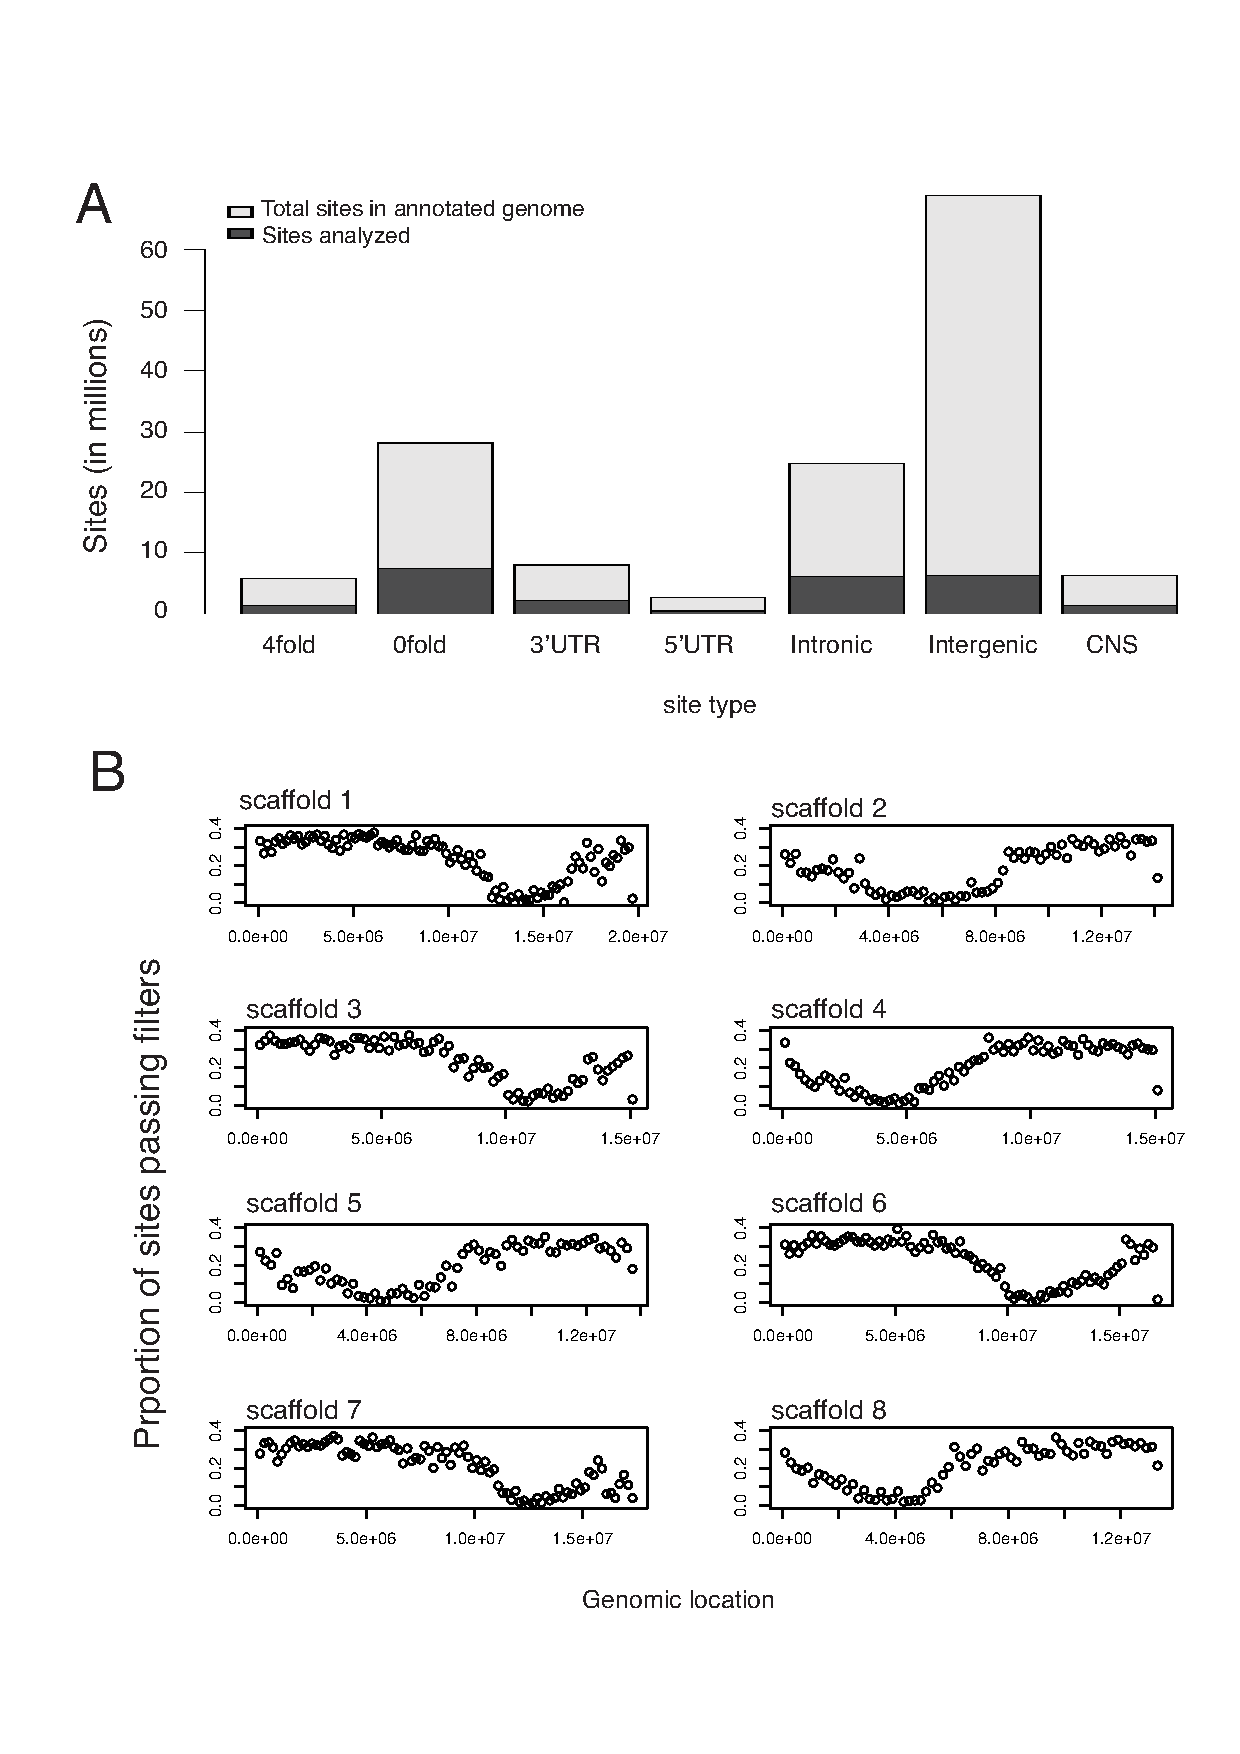
\includegraphics[width=\linewidth]{Ch2FigS1}
    \caption{\textbf{Coverage after filtering, across the genome.} A) The number of annotated sites in each category across the genome (light grey), and the number of sites that pass our filters and were used in analysis (dark grey). B) Proportion of sites that pass filters, calculated in 200kb windows, as a function of genomic position.}
    \label{fig:figS1}
\end{figure}

\begin{figure}[h!]
      \centering
       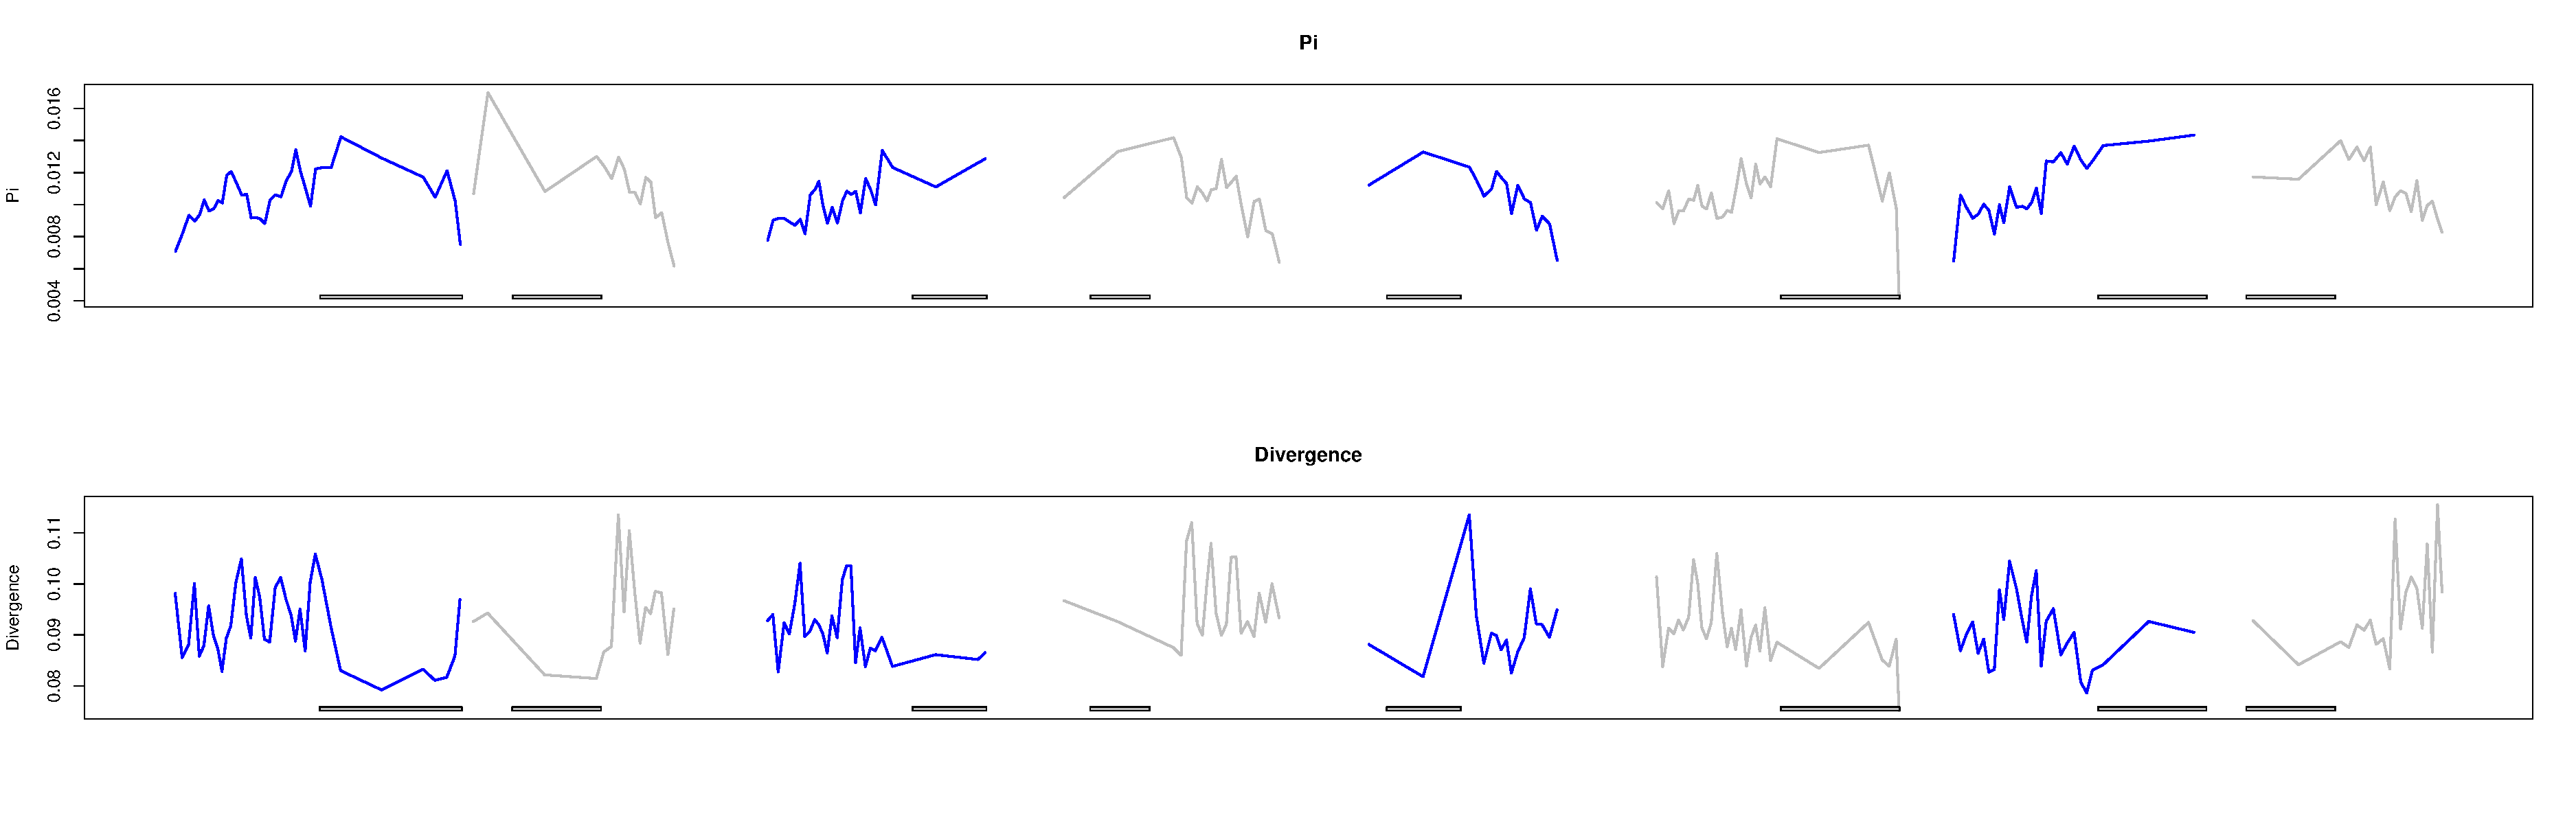
\includegraphics[width=\linewidth]{Ch2FigS2.pdf}
    \caption{\textbf{Pairwise diversity and divergence at 4-fold degenerate sites across the entire genome.} Statistics were calculated in windows of 5,000 SNPs. Individual lines alternating between grey and blue represent chromosomes. The location of the centromere on each chromosome is indicated by the grey box along the x-axis.}
    \label{fig:figS2}
\end{figure}

\begin{figure}[h!]
      \centering
       \includegraphics[width=\linewidth]{Ch2FigS3}
    \caption{\textbf{Coding density versus 4-fold degenerate diversity across the genome.} Each point represents one 10 kb window. Black points represent windows that do not overlap centromeres while grey points represent windows that do overlap centromeres. There is a slight negative correlation between diversity and coding density both with and without centromeric windows}
    \label{fig:figS3}
\end{figure}

\begin{figure}[h!]
      \centering
       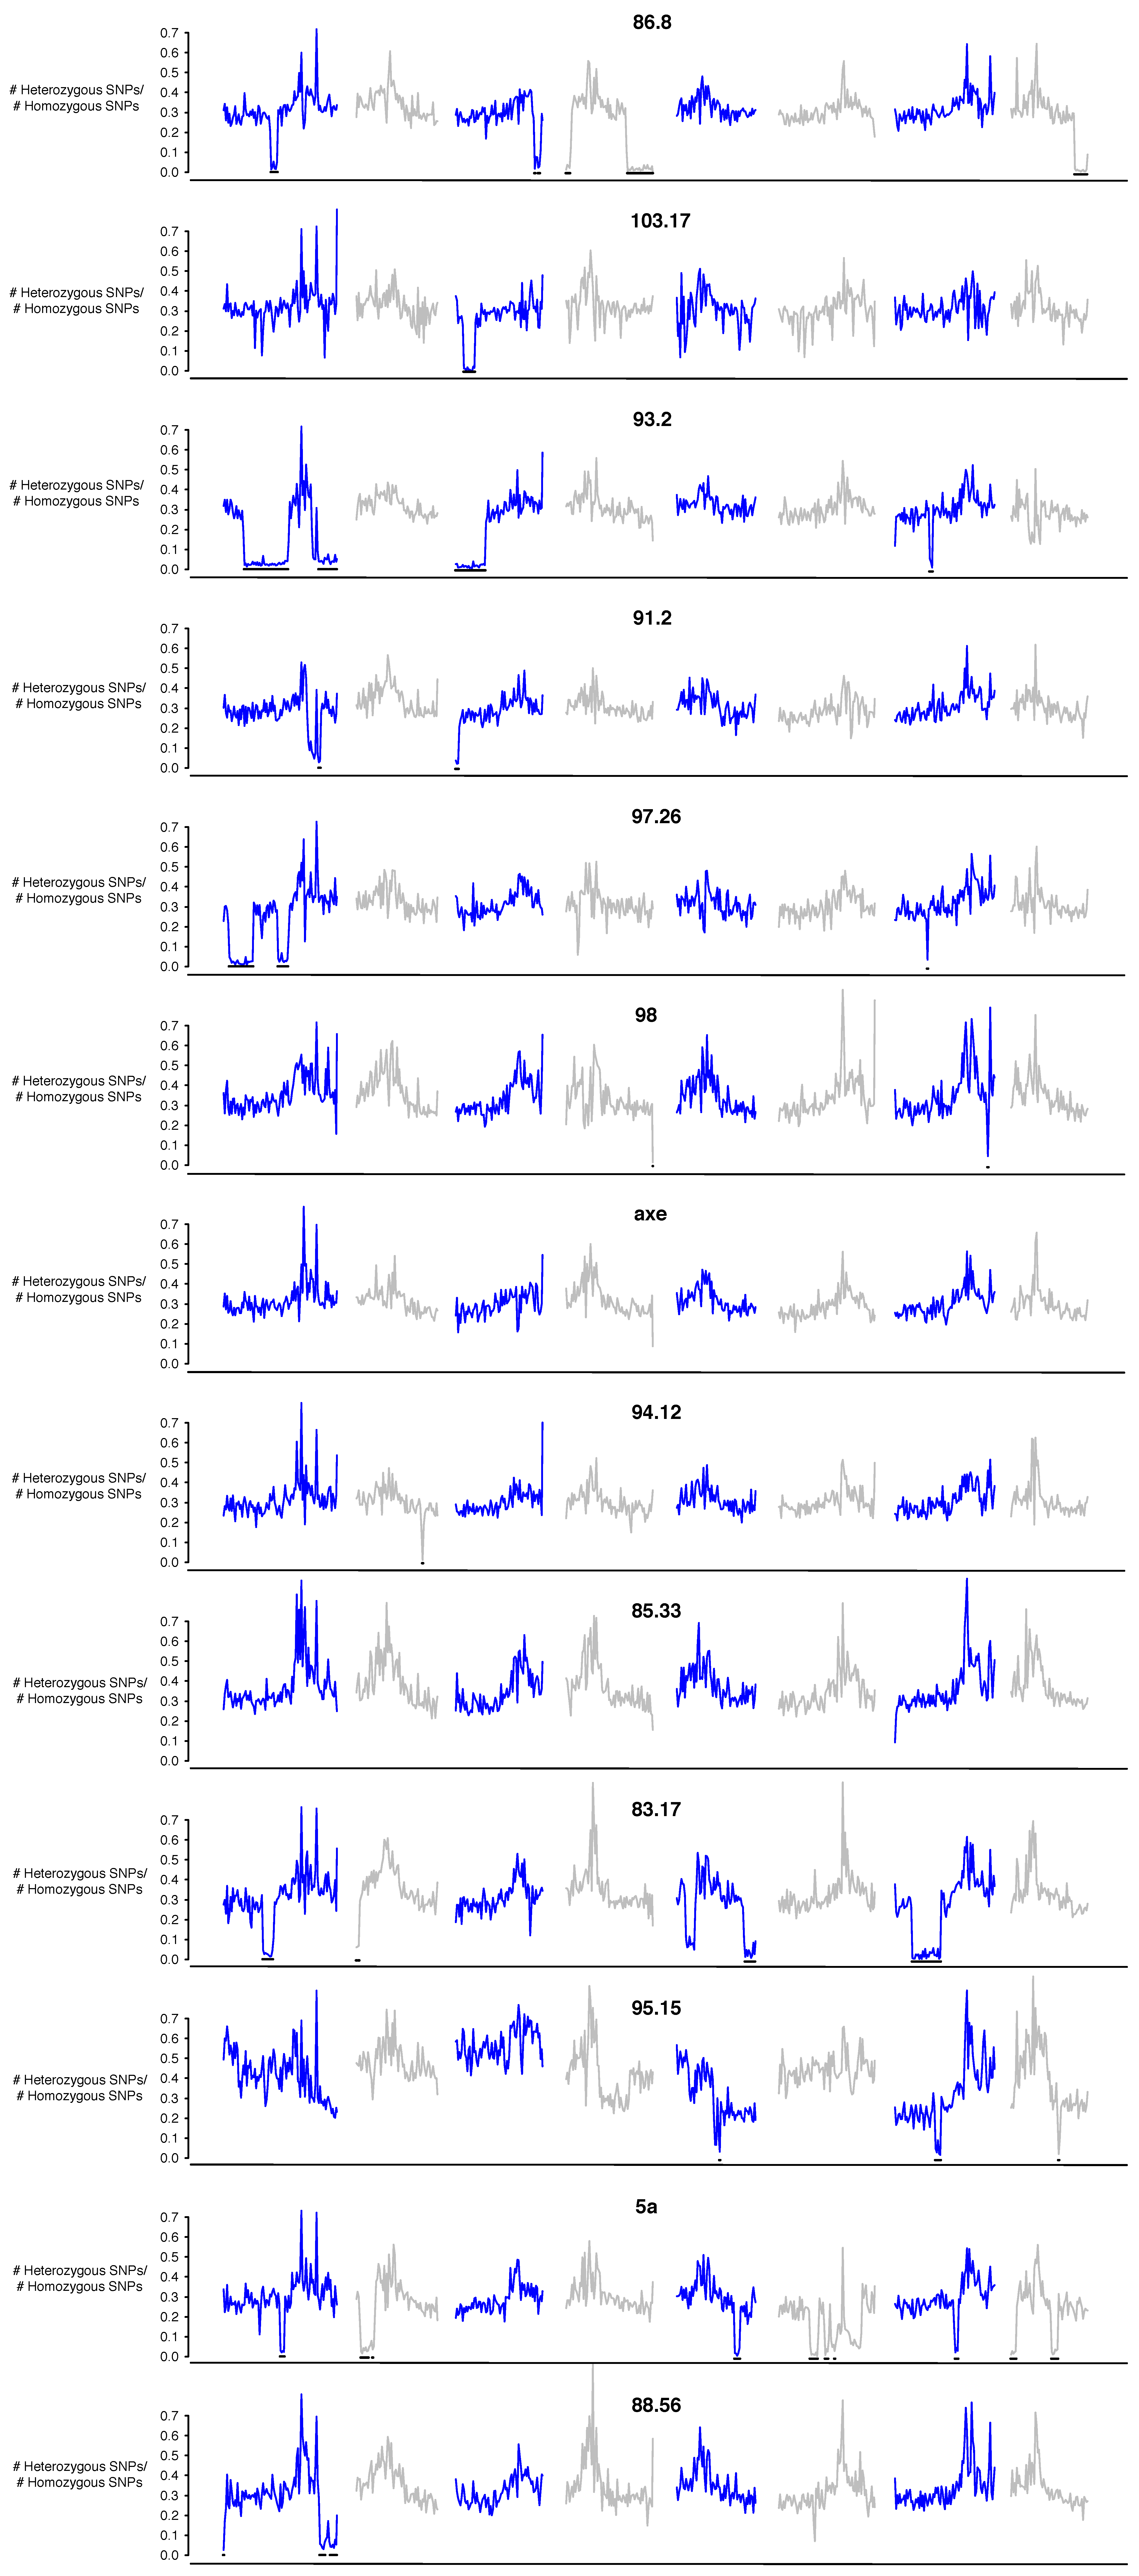
\includegraphics[scale=0.1]{Ch2FigS4}
    \caption{\textbf{Regions of identity by descent in each sample.} The ratio of heterozygous to homozygous calls at sites that are polymorphic across individuals (in 200kb windows) plotted against position across the genome. Each sample is plotted separately and identified by sampled IDs. Individual lines alternating between grey and blue represent chromosomes. Regions of IBD were defined as windows where FIS was greater than 0.5 and are indicated by black lines along the x-axis. At most 3 regions of IBD overlap across all individuals. This occurs near the end of chromosome 1.}
    \label{fig:figS4}
\end{figure}

\begin{figure}[h!]
      \centering
       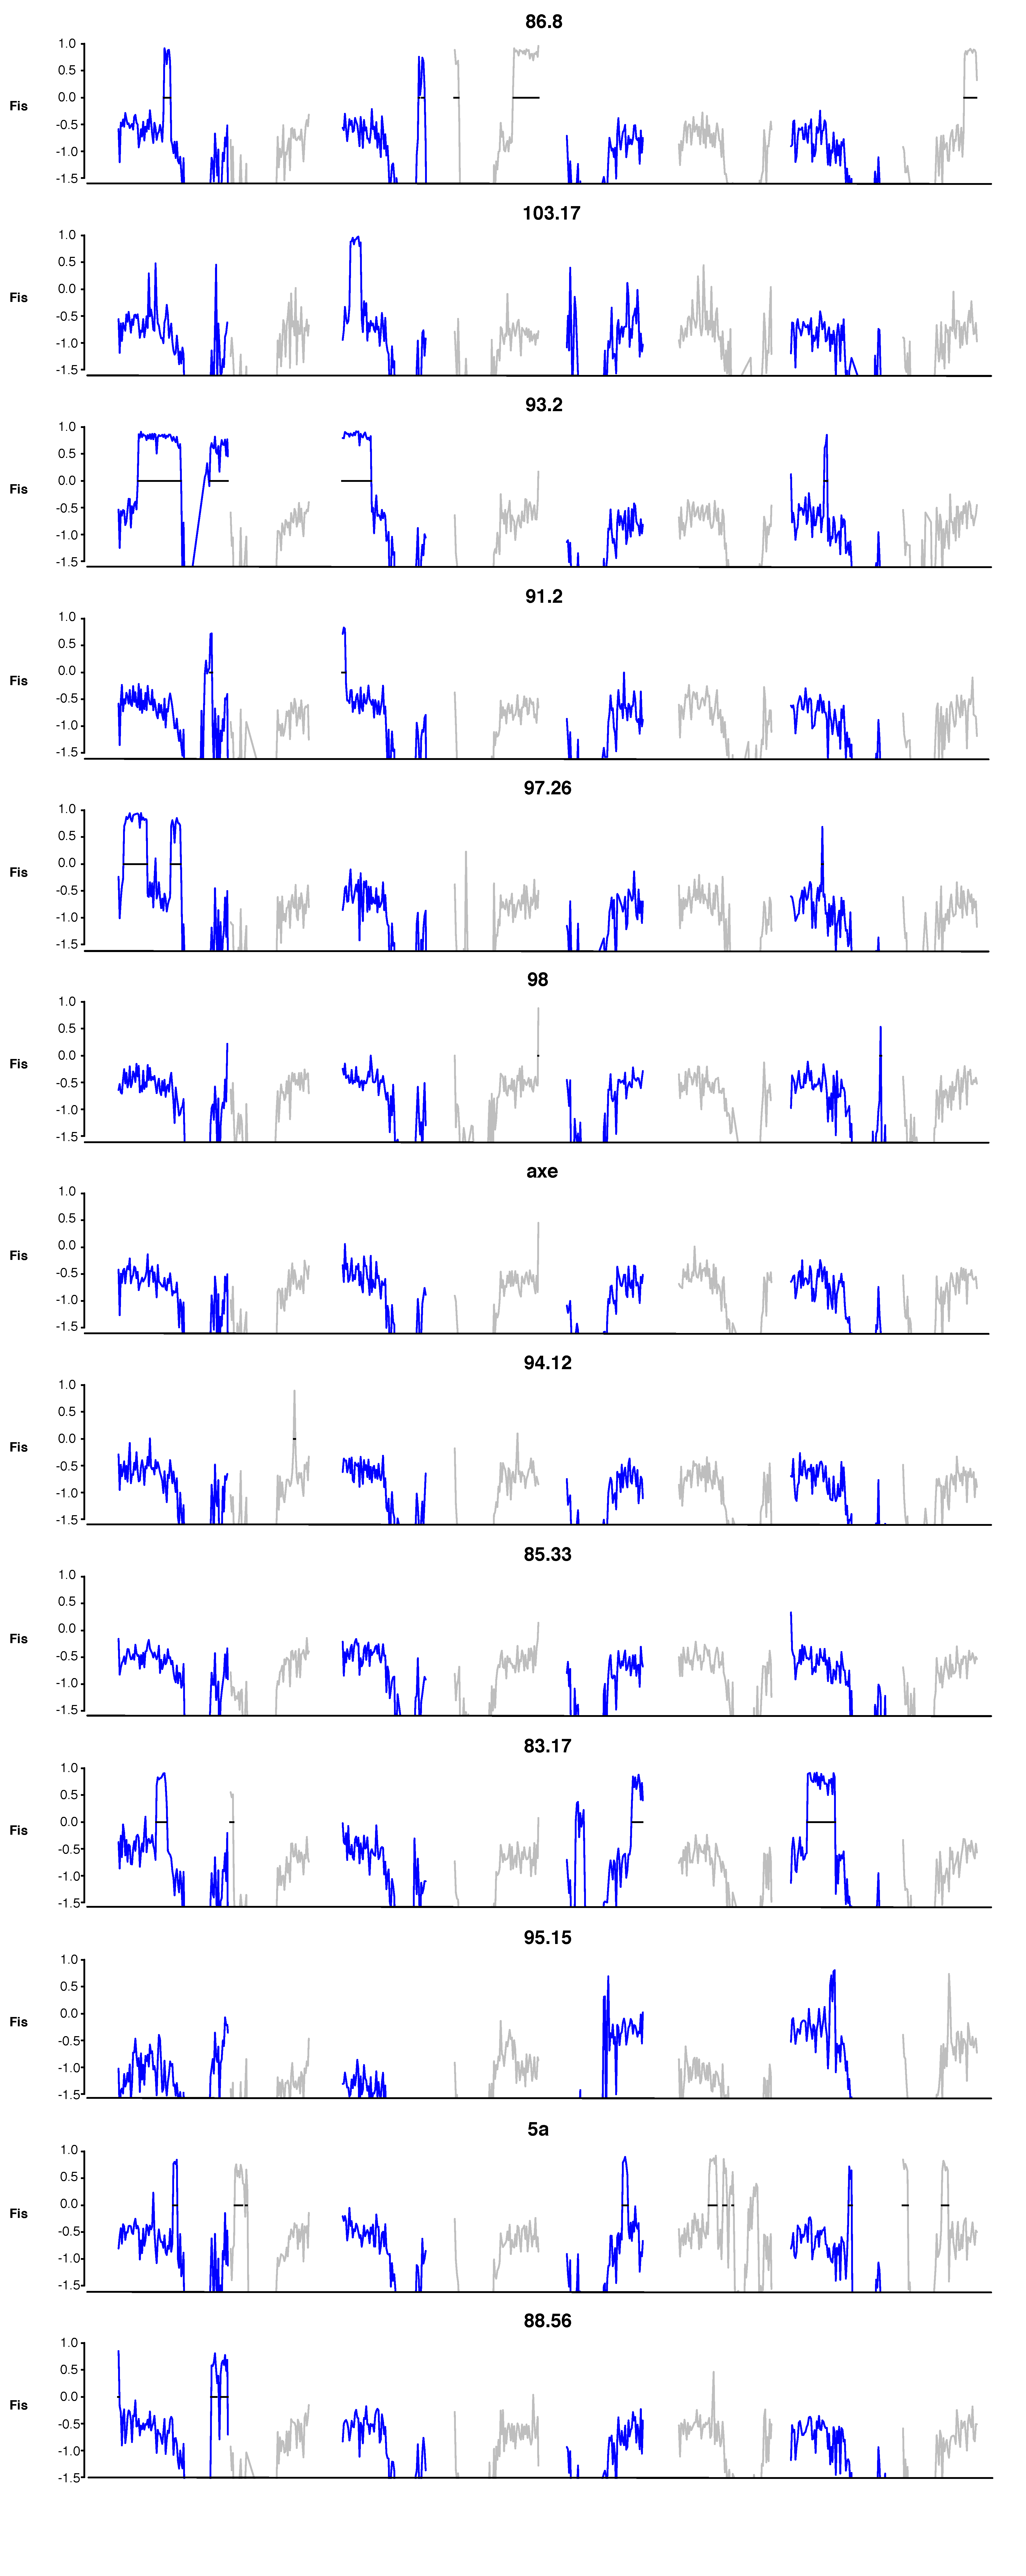
\includegraphics[scale=0.1]{Ch2FigS5}
    \caption{\textbf{FIS in windows across the genome in each sample.} FIS in 200kb windows is plotted across the genome. Each sample is plotted separately and identified by sample IDs. Individual lines alternating between grey and blue represent chromosomes. Regions of IBD were defined as windows where FIS was greater than 0.5 and are indicated by black lines along the 0 line of the y-axis.}
    \label{fig:figS5}
\end{figure}

\begin{figure}[h!]
      \centering
       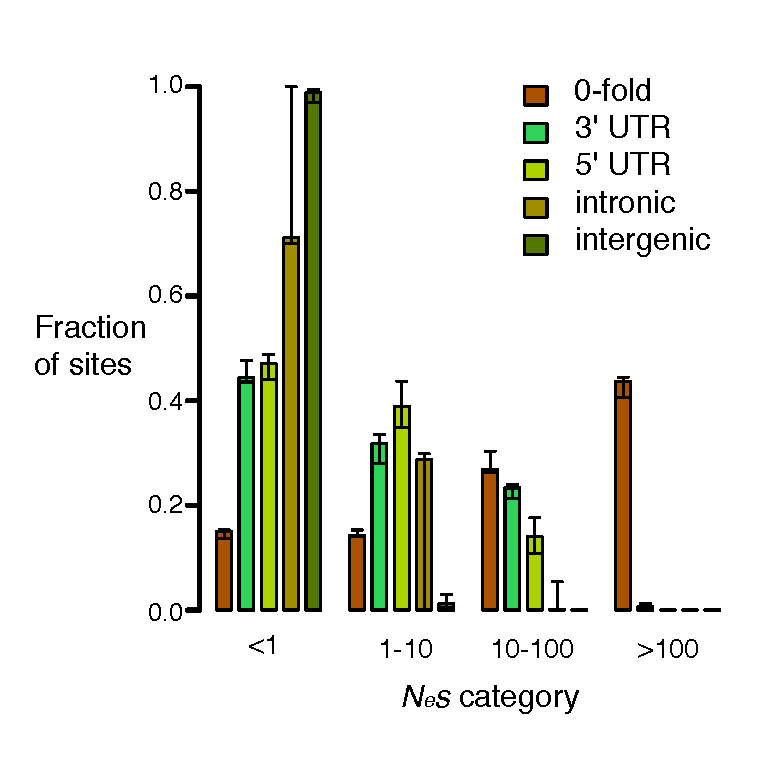
\includegraphics[width=\linewidth]{Ch2FigS6}
    \caption{\textbf{DFE-alpha results using all alleles, including IBD regions.} The distribution of fitness effects for 0-fold degenerate, 3’ and 5’ UTR, intronic, and intergenic sites are shown. For this analysis the genotyping calls were filtered as described in the methods, but the data was not downsampled in regions of IBD identified in Fig.~\ref{fig:figS4}.}
    \label{fig:figS6}
\end{figure}

\begin{figure}[h!]
      \centering
       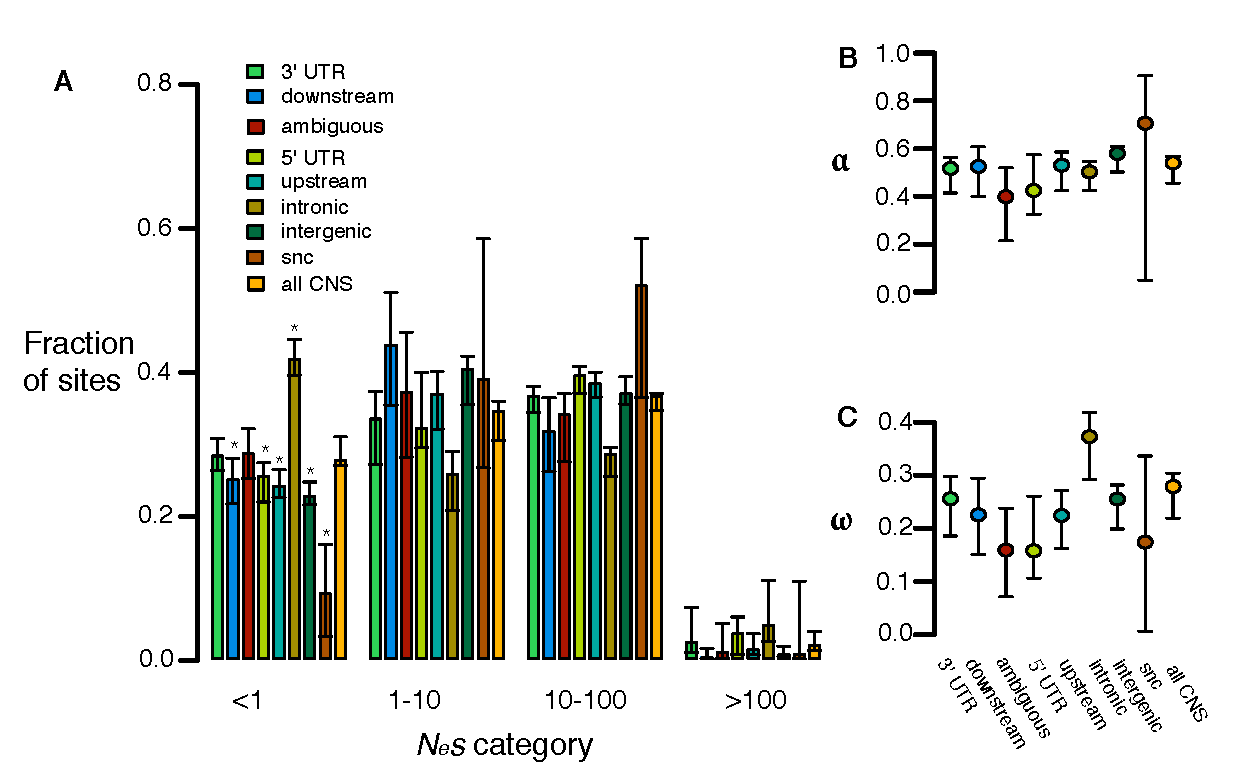
\includegraphics[width=\linewidth]{Ch2FigS7}
    \caption{\textbf{Estimates of positive and negative selection on different categories of CNSs.} A) Distribution of fitness effects. Stars indicate categories in which the fraction of nearly neutral sites was significantly different from the pooled sets of CNSs by a randomization test. B) $\alpha$ and C) $\omega$ for each category. Error bars indicate 95\% CIs from 200 bootstraps.}
    \label{fig:figS7}
\end{figure}

\begin{figure}[h!]
      \centering
       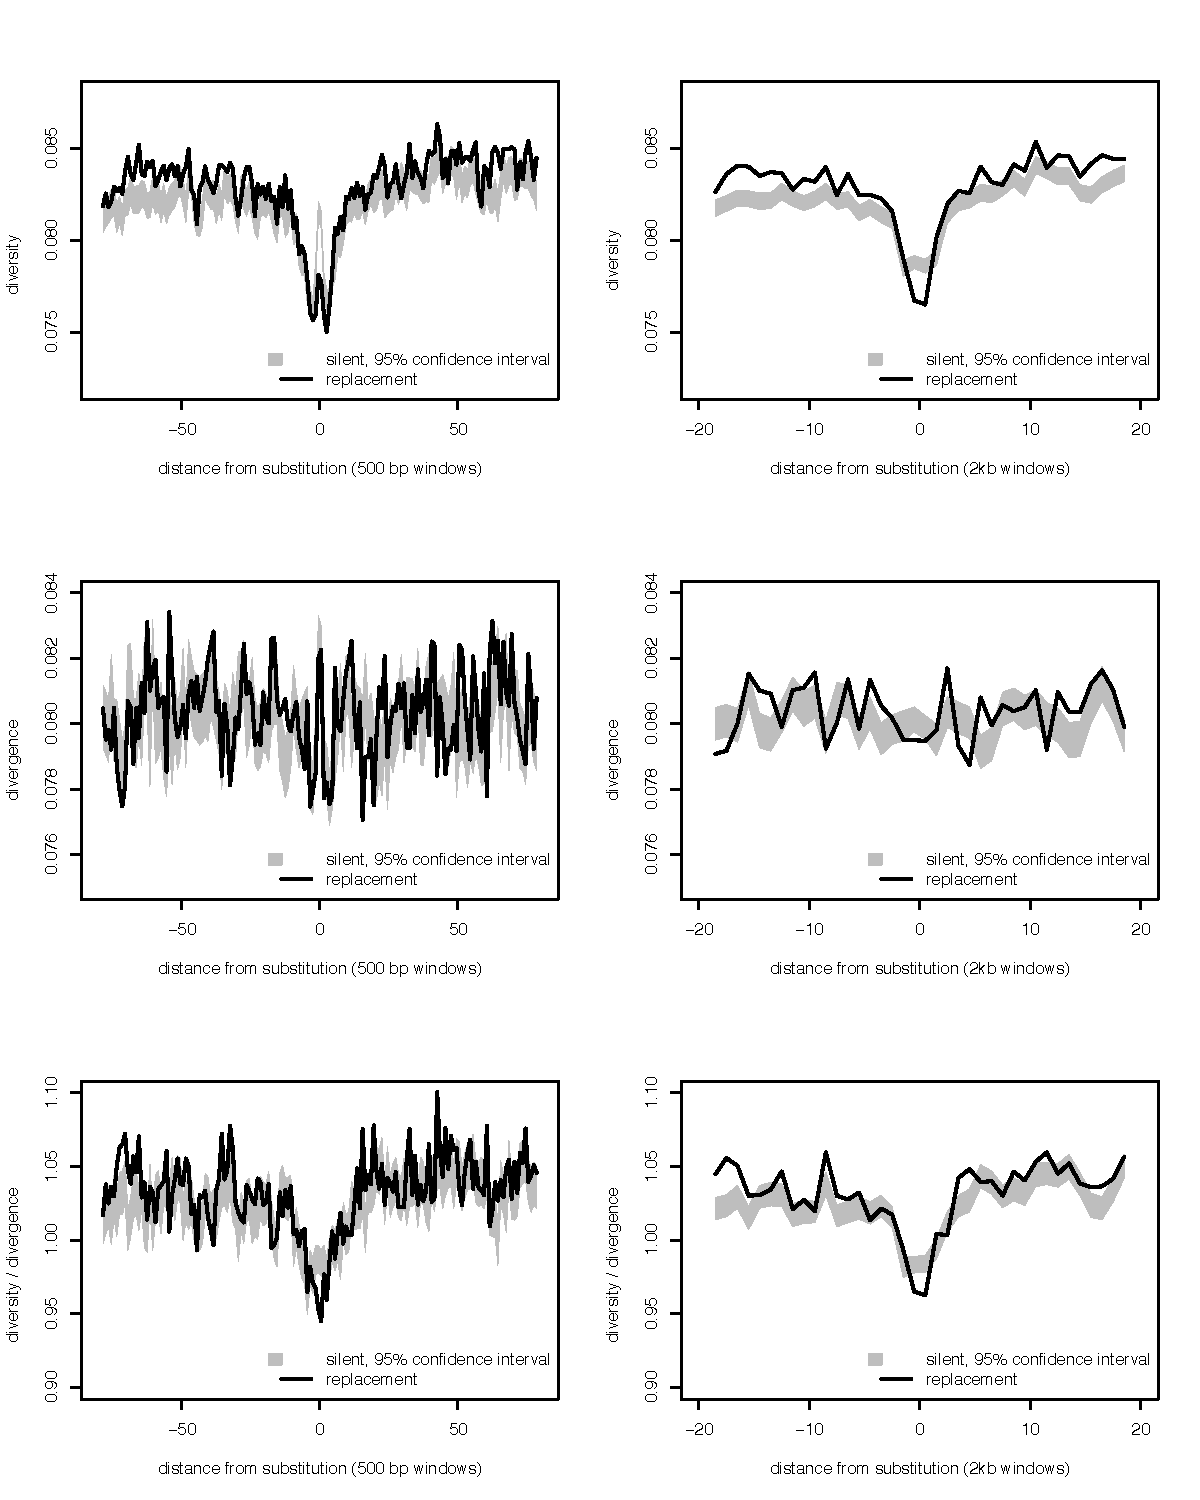
\includegraphics[width=\linewidth]{Ch2FigS8}
    \caption{\textbf{Robustness of sweep analysis to different window sizes.} This panel shows the results of our scans for recurrent selective sweeps using alternative window sizes: 500bp on left and 2kb on right. Otherwise, the methods are the same as described previously.}
    \label{fig:figS8}
\end{figure}

\begin{figure}[h!]
      \centering
       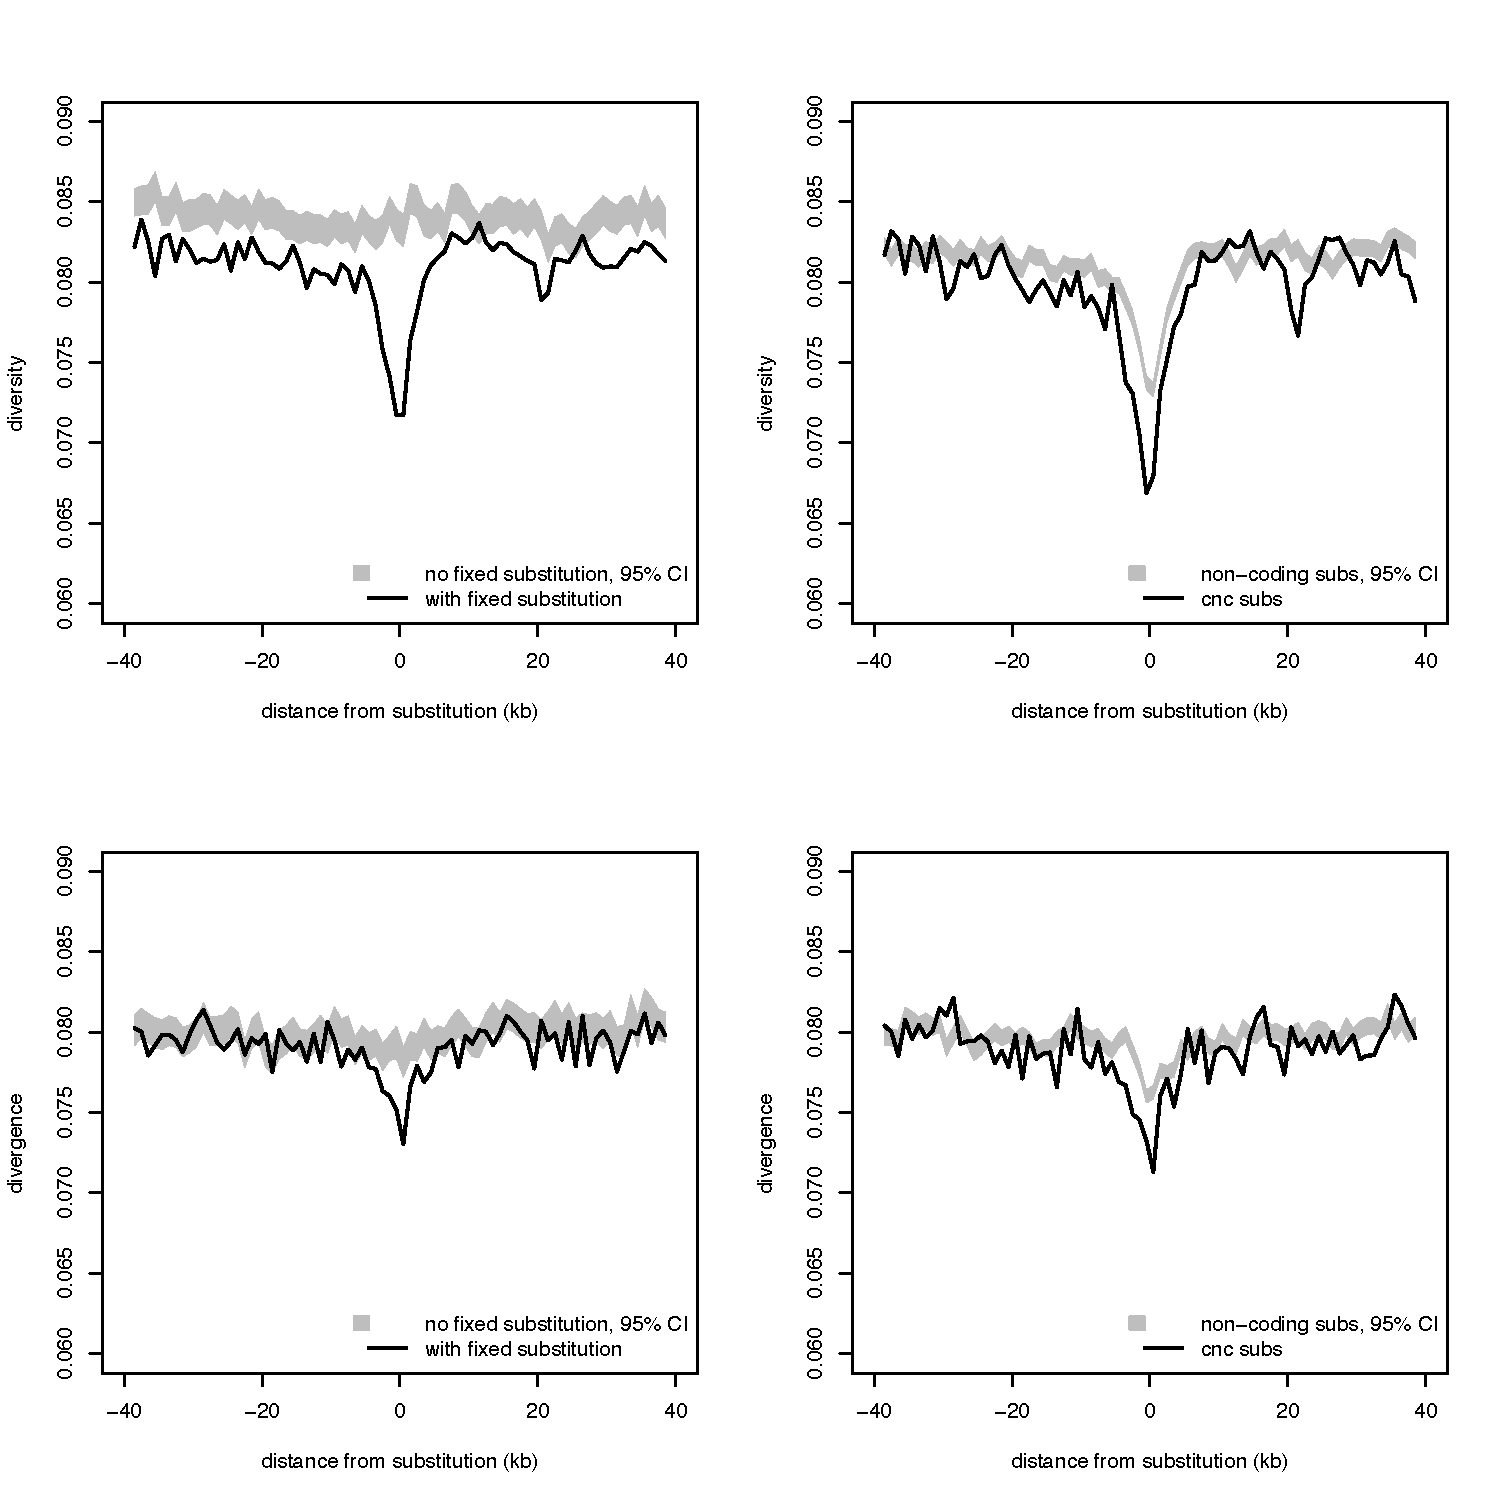
\includegraphics[width=\linewidth]{Ch2FigS9}
    \caption{\textbf{Additional diversity and divergence data for sweeps around substitutions in conserved noncoding regions.} The left panels show diversity at 4-fold degenerate sites and divergence at 4-fold degenerate sites around substitutions in conserved non-coding sequence (black lines) and non-conserved intergenic sequence (gray shading represents 95\% confidence intervals). The right panels show the same information for diversity and divergence at 4-fold degenerate sites around conserved noncoding sequences containing fixed substitutions (black lines) and conserved noncoding sequences without fixed substitutions (gray shading represents 95\% confidence intervals).}
    \label{fig:figS9}
\end{figure}

\begin{figure}[h!]
      \centering
       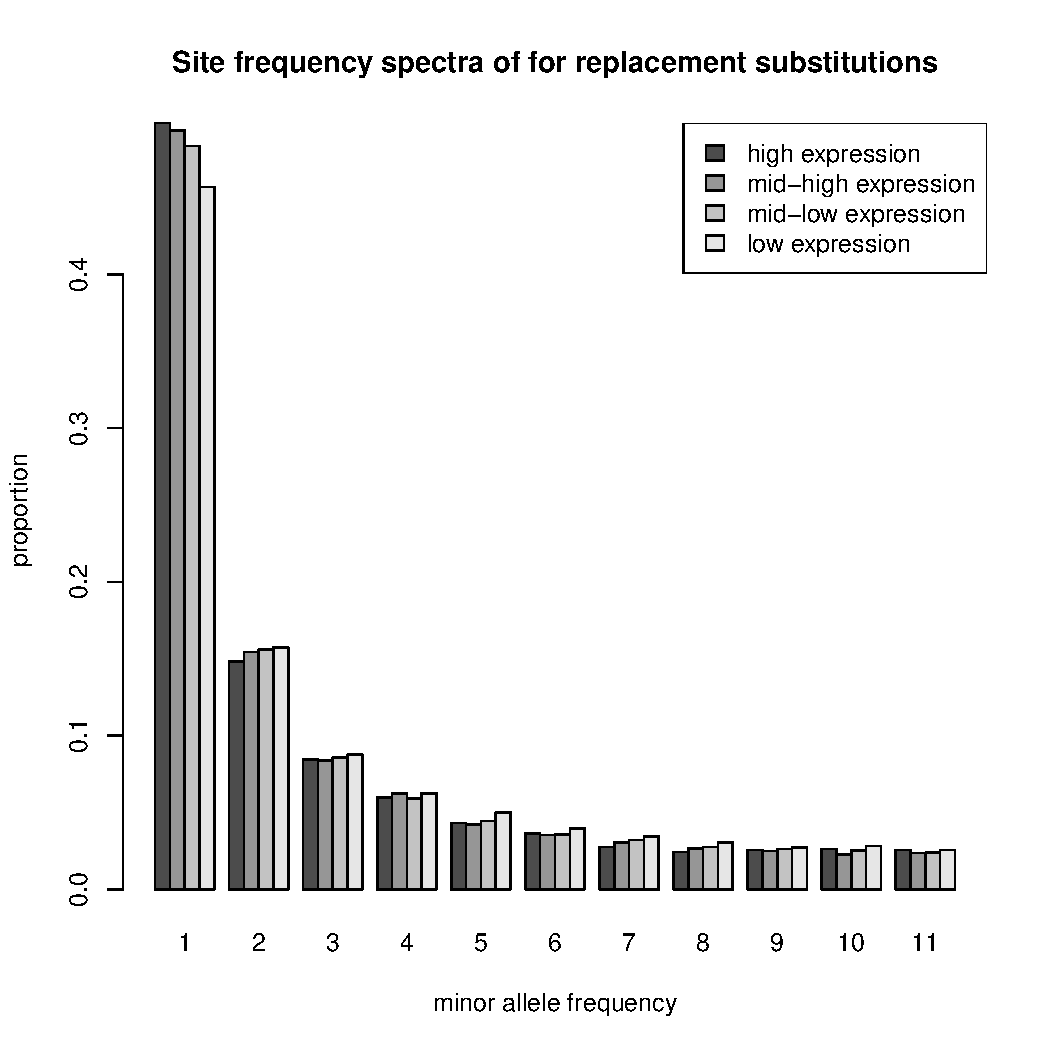
\includegraphics[width=\linewidth]{Ch2FigS10}
    \caption{\textbf{Allele frequency spectra of replacement sites in genes with different expression levels.}}
    \label{fig:figS10}
\end{figure}

\begin{figure}[h!]
      \centering
       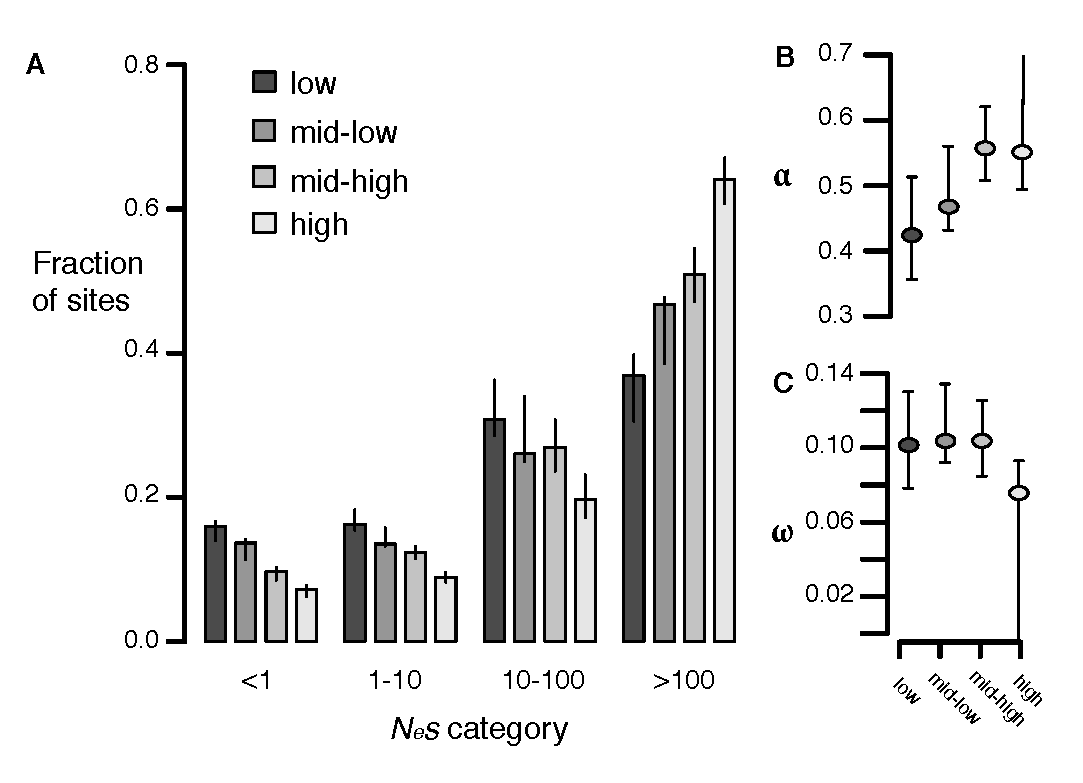
\includegraphics[width=\linewidth]{Ch2FigS11}
    \caption{\textbf{Estimates of negative and positive selection on 0-fold sites in genes of varying expression level.} Data from this figure was generated using the divergence estimates from the whole genome alignments (as in Fig.~\ref{fig:fig1}) rather than divergence from PAML estimates (as in Fig.~\ref{fig:fig4}). Here AFS from 0-fold sites were compared to 4-fold sites, rather than non-synonymous to synonymous sites as in Fig.~\ref{fig:fig4}. A) The proportion of sites found in each bin of purifying selection strength, separated by expression level. B) The proportion of divergent sites fixed by positive selection and C) The rate of adaptive substitution relative to neutral divergence. Error bars represent 95\% bootstrap confidence intervals.}
    \label{fig:figS11}
\end{figure}

Table S1
Sampling locations of each sample.

Table S2
Allele frequency spectra, summary of diversity statistics, and DFE-alpha model parameters for each site category. 


\setlength{\parindent}{0ex}
\setlength{\parskip}{2ex}

%\chapter{Association mapping reveals the role of mutation-selection balance in the maintenance of genomic variation for gene expression.}
\chapter{Mutation-selection balance maintains gene expression variation}

\section{Abstract}
The evolutionary forces that maintain genetic variation for quantitative traits within populations remain poorly understood. One hypothesis suggests that variation is maintained by a balance between new mutations and their removal by selection and drift. Theory predicts that this mutation-selection balance will result in an excess of low-frequency variants and a negative correlation between minor allele frequency and selection coefficients. Here, we test these predictions using the genetic loci associated with total expression variation (eQTLs) and allele-specific expression variation (aseQTLs) mapped within a single population of the plant \textit{Capsella grandiflora}. In addition to finding eQTLs and aseQTLs for a large fraction of genes, we show that alleles at these loci are rarer than expected and exhibit a negative correlation between phenotypic effect size and frequency. Overall, our results show that the distribution of frequencies and effect sizes of the loci responsible for local expression variation within a single, outcrossing population are consistent with mutation-selection balance.

\section{Introduction}
Genetic variation for quantitative traits persists within populations despite the expectation that prevalent stabilizing selection will reduce genetic variance. One hypothesis suggests that variation is maintained by a balance between new mutations and their removal by selection and drift, resulting in an excess of low-frequency variants and a negative correlation between minor allele frequency and selection coefficients \citep{Haldane1927-pj}. While studies of allele frequency spectra show that purifying selection is often prevalent in genomic sequence \citep{Kousathanas2011-bf,Zhu2011-gf,Williamson2014-tf}, little is known about how the genetic variants under selection relate to phenotype, and ultimately, how phenotypic variation is maintained within populations. Association mapping can identify specific loci influencing phenotype providing candidates for further analysis of selection \citep{Lee2014-pi}. In particular, mapping the local regulatory variants that affect gene expression can identify a large number of genetic loci that affect phenotype. Additionally, mapping the genetic basis of gene expression will answer questions about the basic biology of gene regulation, for example, by testing predictions that conserved non-coding sequences (‘CNSs’) are constrained because they have regulatory function \citep{Haudry2013-qe}.

Early eQTL studies mapped expression divergence between two lines, finding that many genes have local expression QTL \citep{Brem2005-gs,Brem2002-cc}. These studies have provided insight into selection on eQTLs; for example,  a correlation between recombination rate and eQTL density implies that background selection is a dominant force acting on expression variation in \textit{Caenorhabditis elegans} \citep{Rockman2010-qm} and a skew towards rare allele frequencies in promoters of genes with eQTLs suggests that purifying selection may act on expression variation \citep{Ronald2007-hf}. However, eQTL studies of population-level genetic variation have thus far been limited to a few study systems \citep{Massouras2012-wq,Pickrell2010-ci,Lappalainen2013-jh,Battle2014-ke,Tung2015-cg} and only one study, in humans, has identified a negative correlation between phenotypic effect size and frequency \citep{Battle2014-ke}. In addition, human eQTL studies have shown that loci expected to be involved in selective sweeps are more likely to be eQTLs than other loci \citep{Kudaravalli2009-gw}, alleles eQTLs that increase expression of a potentially deleterious coding SNP are under stronger purifying selection than those that do not \citep{Lappalainen2011-tw}, and eQTL allele frequencies within populations are linked to local adaptation \citep{Fraser2013-rm,Ye2013-fx}. To date, eQTL studies in plants have used genetic crosses \citep{Potokina2008-bk,West2007-fm,Bolon2014-km} or species-wide samples \citep{Gan2011-xv, Zhang2011-ut,Fu2013-kf}, making it difficult to distinguish evolutionary forces acting within and between populations. In sum, we currently lack comprehensive tests of selection on within-population eQTLs in any system, especially in plants.

Here, we map local regulatory loci affecting expression in 99 members of a single large population of \textit{Capsella grandiflora} (Brassicaceae), an obligate outcrosser. As might be expected from its large $N_{e}$ and relative lack of population structure, purifying and positive selection are strong in \textit{C. grandiflora}\citep{Williamson2014-tf,St_onge2011-jz}, making it an ideal system for investigating the maintenance of genetic variation in the face of selection 

\section{Results and Discussion}
We sequenced 22,895,738,517 100bp paired-end reads of DNA from 188 individuals, with a median of 119,321,591 reads per individual. Of these reads, a median of 93\% mapped per individual (range: 51\%-93\%, the two individuals with \textless 80\% were not sampled for RNAseq). We called 9,526,786 SNPs with a mean depth of 45 reads per individual. Linkage disequilibrium between SNPs decays rapidly: mean $r^{2}$ between SNPs less than 10bp apart is 0.25, and this decays to 0.12 within 100bp (Fig.~\ref{fig:3figS1}). An analysis of population structure \citep{Raj2014-im} found that the maximum likelihood number of populations was K=1, suggesting no widespread structure. We measured genome-wide gene expression in 99 of these individuals using RNAseq from young leaf tissue, generating 4,988,540,400 100bp paired-end RNAseq reads with a median of 49,549,336 reads per individual (range: 42,627,096-106,283,910). Of these, a median of 94\% (range: 89-95\%) mapped to genes. 

\begin{figure}[!ht]
      \centering
       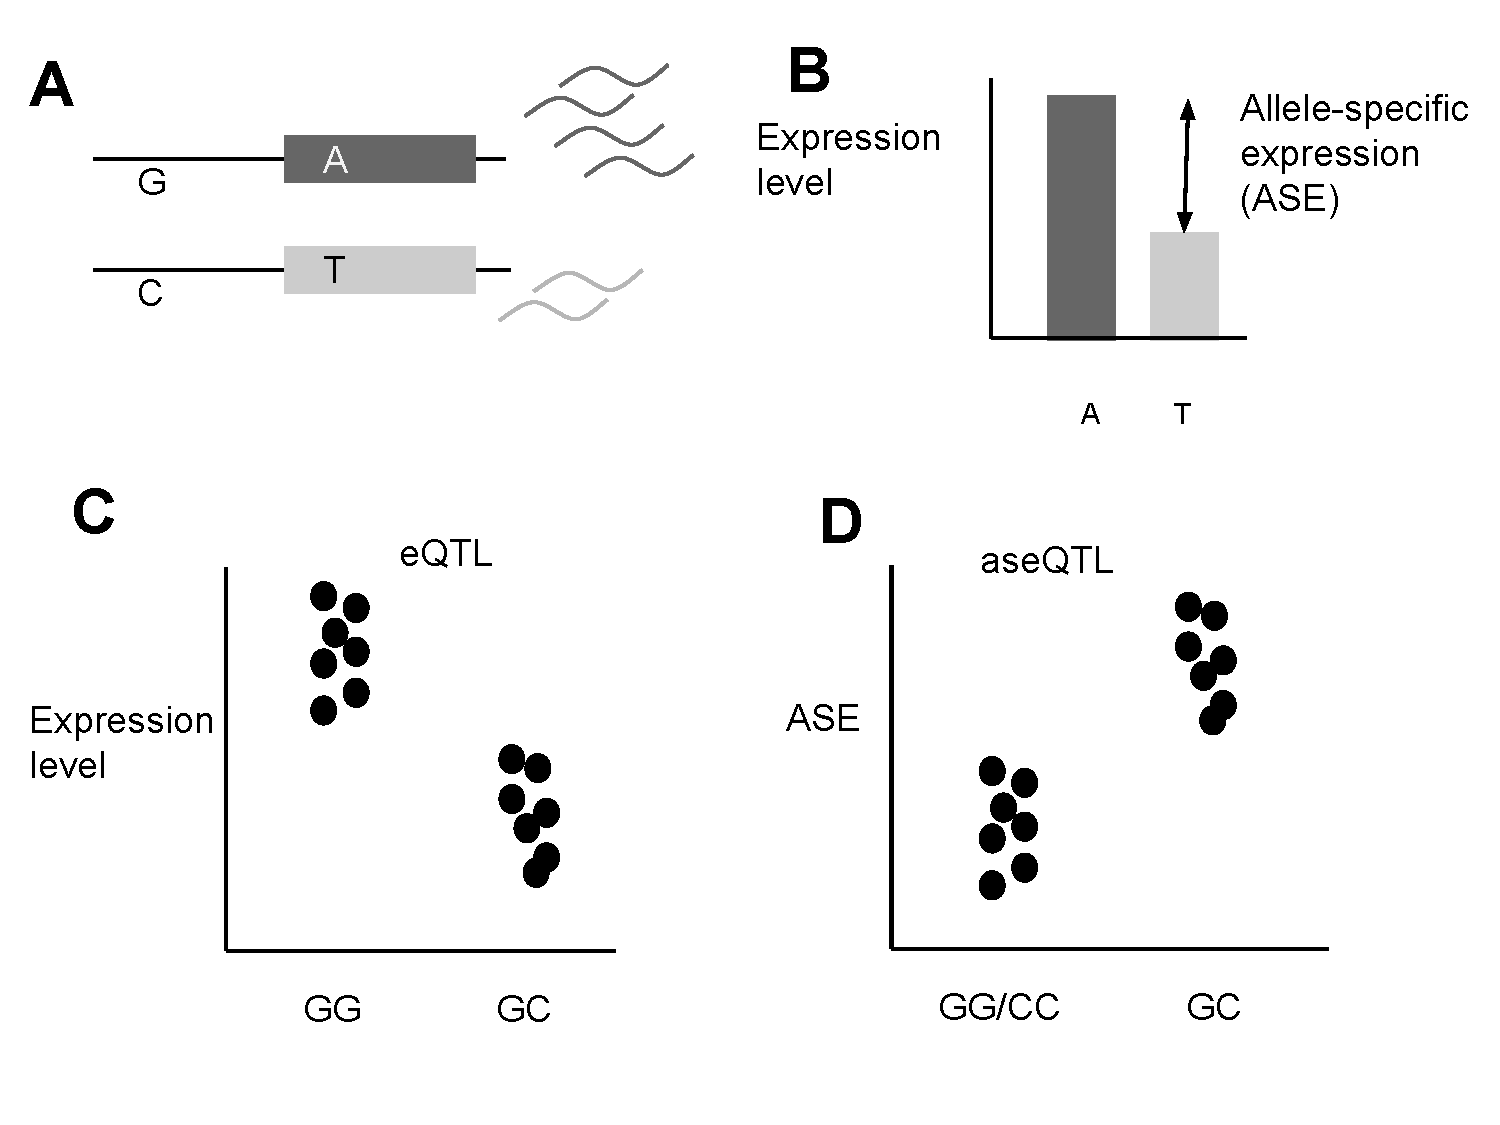
\includegraphics[width=\linewidth]{Ch3Fig1}
    \caption{\textbf{Detecting eQTLs and aseQTLs} A) A gene model for an individual that is heterozygous at a regulatory locus (G/T) and at an informative coding site (A/T). The G allele increases expression relative to the C allele, B) causing increased allelic expression of the reads carrying the A allele at the informative heterozygous site. We refer to this difference in allelic expression as “ASE”. C) eQTLs are detected when there is a significant difference in total gene expression between individuals (represented by black circles) that are homozygous for the common allele of a SNP and individuals that are heterozygous at that SNP. D) aseQTLs are detected when there is a significant difference in ASE between individuals that are heterozygous at a SNP and homozygous for either allele at that SNP.}
    \label{fig:3fig1}
\end{figure}


We mapped eQTLs by performing Mann-Whitney U tests comparing expression between individuals homozygous for the most common allele at a given SNP and those heterozygous at that SNP, for all SNPs within 5kb of the transcription start and end sites (Fig.~\ref{fig:3fig1}). We omitted rare homozygotes from the analysis because most local regulation acts additively in \textit{cis} (12) and low sample sizes for rare variants reduce power. Out of 5,507,316 SNPs tested against the expression of 18,692 genes, 39,628 SNPS are significantly associated with expression of 6,624 nearby genes (FDR = 0.1, p \textless 8.2 x 10$^{-4}$, Fig.~\ref{fig:3figS2} A). These SNPs often clustered locally (Fig.~\ref{fig:3figS3} A,B), as would be expected if non-causal SNPs are in linkage disequilibrium with causal SNPs. Patterns of functional enrichment in human eQTLS suggest that SNPs most strongly associated with expression are more likely causal than those showing weaker associations \citep{Lappalainen2013-jh}, so to prevent variation in linkage disequilibrium from affecting subsequent analyses while increasing the likelihood of retaining causal SNPs, we chose the most significantly associated SNP for each gene for further analysis (N = 6,624). While there are likely multiple causal eQTLs for many genes, choosing one significant SNP per gene allows us to generate a large independent sample of eQTLs for further analysis.

If eQTLs act in \textit{cis}, heterozygous eQTLs will cause allele-specific expression (ASE), providing an additional signature of regulatory variation. We measured ASE within individuals by calculating the mean expression difference between alleles, standardized for sequencing depth. We then mapped QTLs for ASE (‘aseQTLs’) by performing Mann-Whitney U tests comparing ASE in individuals that were homozygous at a local SNP and those that were heterozygous at that SNP (Fig.~\ref{fig:3fig1}). We excluded coding SNPs from this analysis because their genotype might confound ASE measurement. Out of 3,966,423 SNPS tested, 26,957 SNPs were significantly associated with ASE of 5,882 nearby genes (FDR = 0.1, p \textless 5.4 x 10$^{-4}$, Fig. ~\ref{fig:3figS2} B). Our analysis did not require a directional effect of SNP genotype on ASE, but 22,436 (83\%) of the noncoding SNPs associated with ASE have higher ASE in heterozygotes, as would be expected if these SNPs control expression in \textit{cis}. We selected the most strongly associated noncoding SNP per gene for further analysis and we also required that ASE had to be higher in heterozygotes at that SNP than homozygotes, leaving 4,580 aseQTLs (Fig.~\ref{fig:3figS2} B). 

SNPs located near the transcription start site (TSS) and in 5’ UTRs were more likely to be eQTLs and aseQTLs than SNPs further away from the gene (Fig.~\ref{fig:3fig2}A), consistent with data from humans and Drosophila \citep{Massouras2012-wq,Pickrell2010-ci,Battle2014-ke}. In addition, CNSs near the TSS were enriched for eQTLs and aseQTLs relative to non-conserved sites (Fig.~\ref{fig:3fig2}A), suggesting that genetic variation within CNSs represents a major source of standing variation in gene expression, although bootstrapped confidence limits for these overlap slightly in aseQTLs. In contrast, CNSs in 5’UTRs were not enriched for eQTLs or aseQTLs, consistent with observations that selection strength is relatively similar in conserved and non-conserved sites in these regions \citep{Haudry2013-qe}. However, the detection of a large number of eQTLs outside of conserved regions suggests that regulatory element turnover is common in Brassicaceae. There were 2,236 genes that had both eQTLs and aseQTLs, significantly more than expected by chance ($X^{2}$ = 471, p \textless 2.2x10-16). Of these 2,236 genes, 411 had the same SNP most significantly associated both with expression and ASE.

\begin{figure}[ht!]
      \centering
       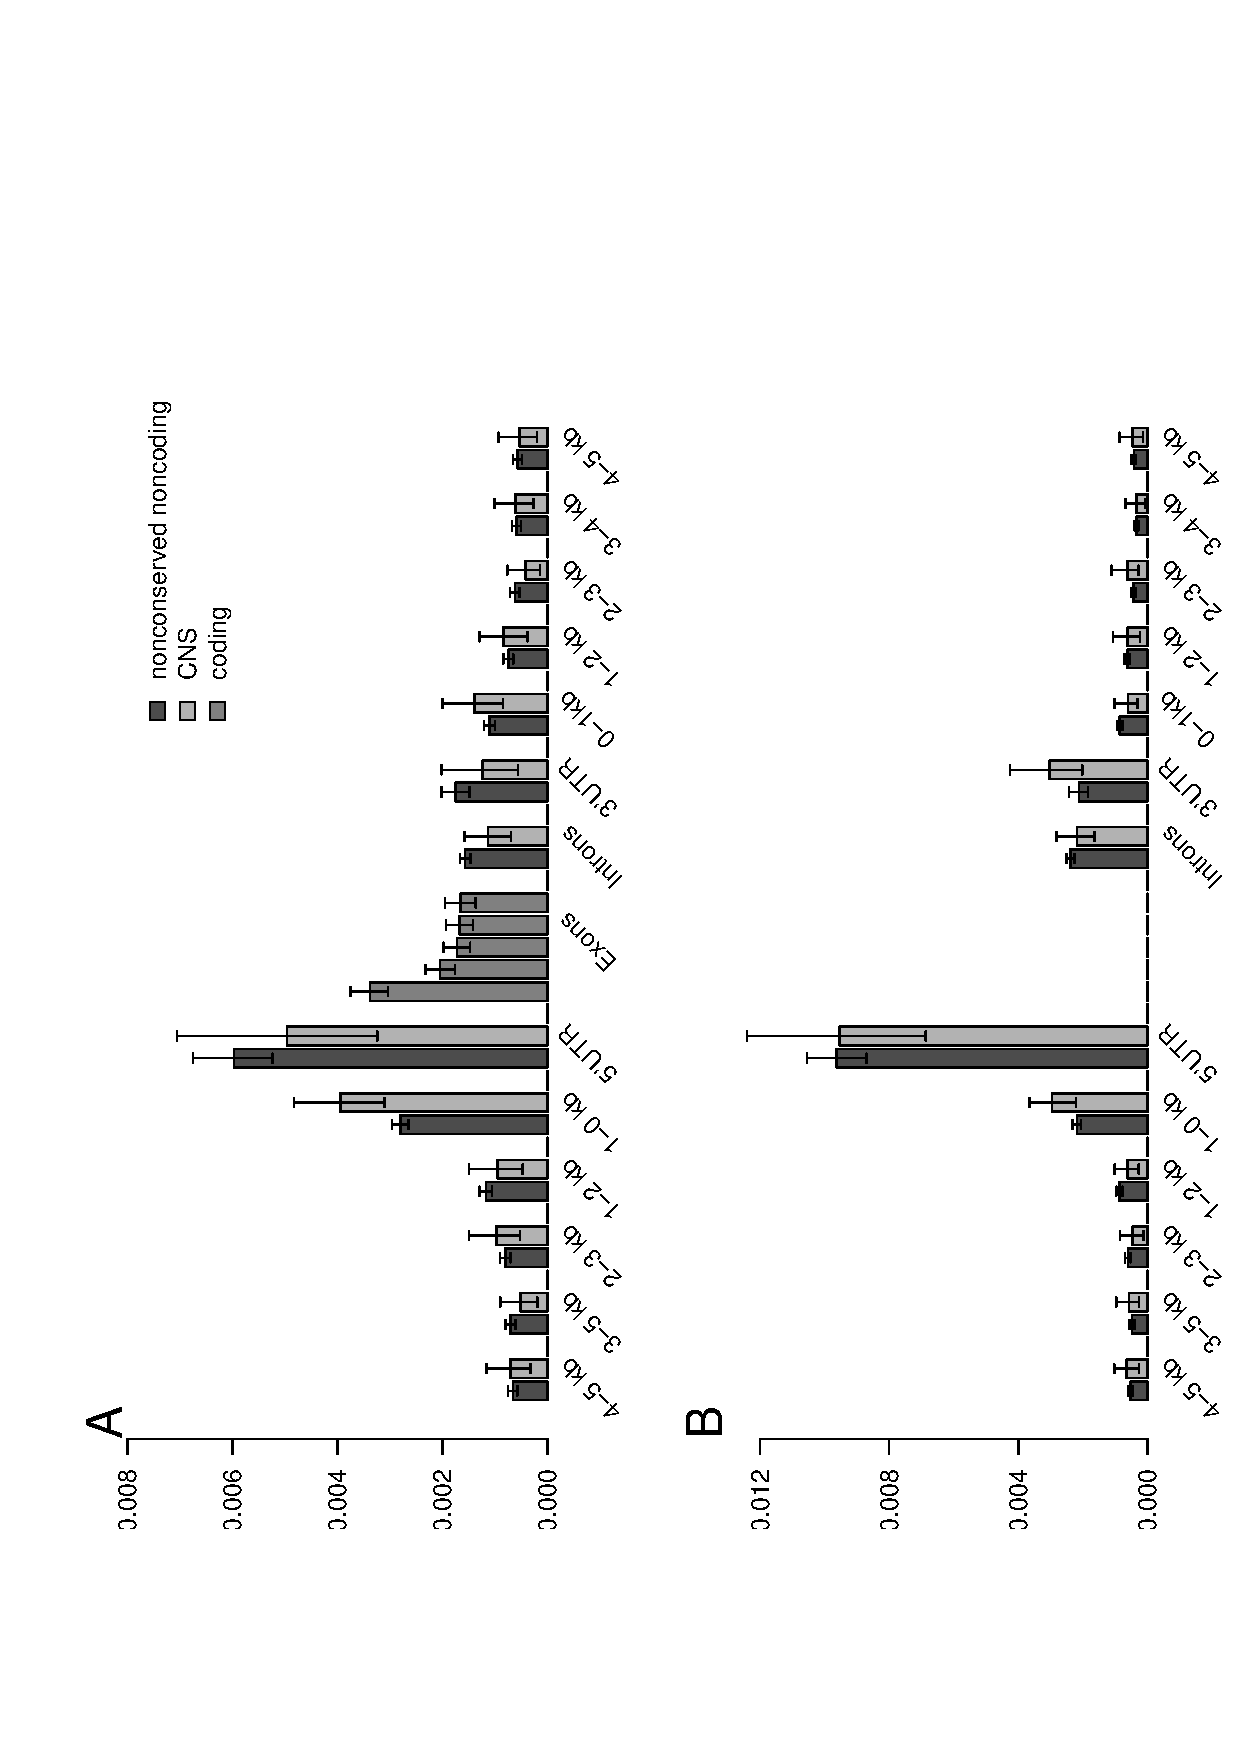
\includegraphics[width=\linewidth]{Ch3Fig2}
    \caption{\textbf{eQTL and aseQTL enrichments by site type.} The proportion of SNPs tested in each category that were found to be eQTLs is plotted on the y axis for A) eQTLs and C) aseQTLs. The exonic classes were determined by splitting the coding sequence of each gene into 5 equally sized pieces. Note that there were no exonic SNPs included in the aseQTL analysis. Error bars show the 95\% confidence intervals from bootstrapping.}
    \label{fig:3fig2}
\end{figure}

Next, we tested eQTLs and aseQTLs for signatures of selection. Purifying selection will reduce the frequency of causal alleles at QTLs, but allele frequency also controls sample size in association studies, affecting QTL detection. Rare alleles have an increased likelihood of false negatives, because of lower power, and false positives, since expression is not normally distributed and an outlier in a small sample is more likely to lead to a positive association than an outlier in a large sample. The increased likelihood of false positives in rare alleles makes evolutionary inferences especially challenging because it mimics the signal of purifying selection.

To generate an appropriate null distribution for QTL allele frequency, we permuted assignments between expression level and genotype for every gene 1000 times and ran eQTL analyses using permuted data. On average, 3,258 SNPs were associated with total expression in our permutations, consistent with an FDR of 0.1, since 39,628 SNPs were associated with the observed data. However, observed eQTLs from un-permuted data were significantly rarer than those found in permuted data (mean N=2,047), consistent with the action of purifying selection (Fig.~\ref{fig:3fig3}A). This observation is conservative, because we have not accounted for reduced power to detect associations on rare alleles. We also investigated permuted aseQTLs, and found on average 3,194 SNPs associated with ASE in each permutation, which is slightly more than expected given our FDR of 10\% (26,597 SNPs were associated with ASE in un-permuted data). As with eQTLs, aseQTLs were significantly rarer than those found in permuted data (Fig.~\ref{fig:3fig3}B). These results hold when we designate a random significantly-associated SNP per gene as the eQTL or aseQTL (Fig.~\ref{fig:3figS4} A,B). In addition, eQTLs and aseQTLs are significantly rarer than permuted eQTLs and aseQTLs when only SNPs 1-5 kb upstream or downstream of genes are considered (Fig.~\ref{fig:3figS5} A,B), and when sites are separated into high and low recombination sets or by substitution type (Fig.~\ref{fig:3figS5} C,D). Thus, the frequency distribution of both eQTLs and aseQTLs is consistent with the predominance of mutation-selection balance.

\begin{figure}[ht!]
      \centering
       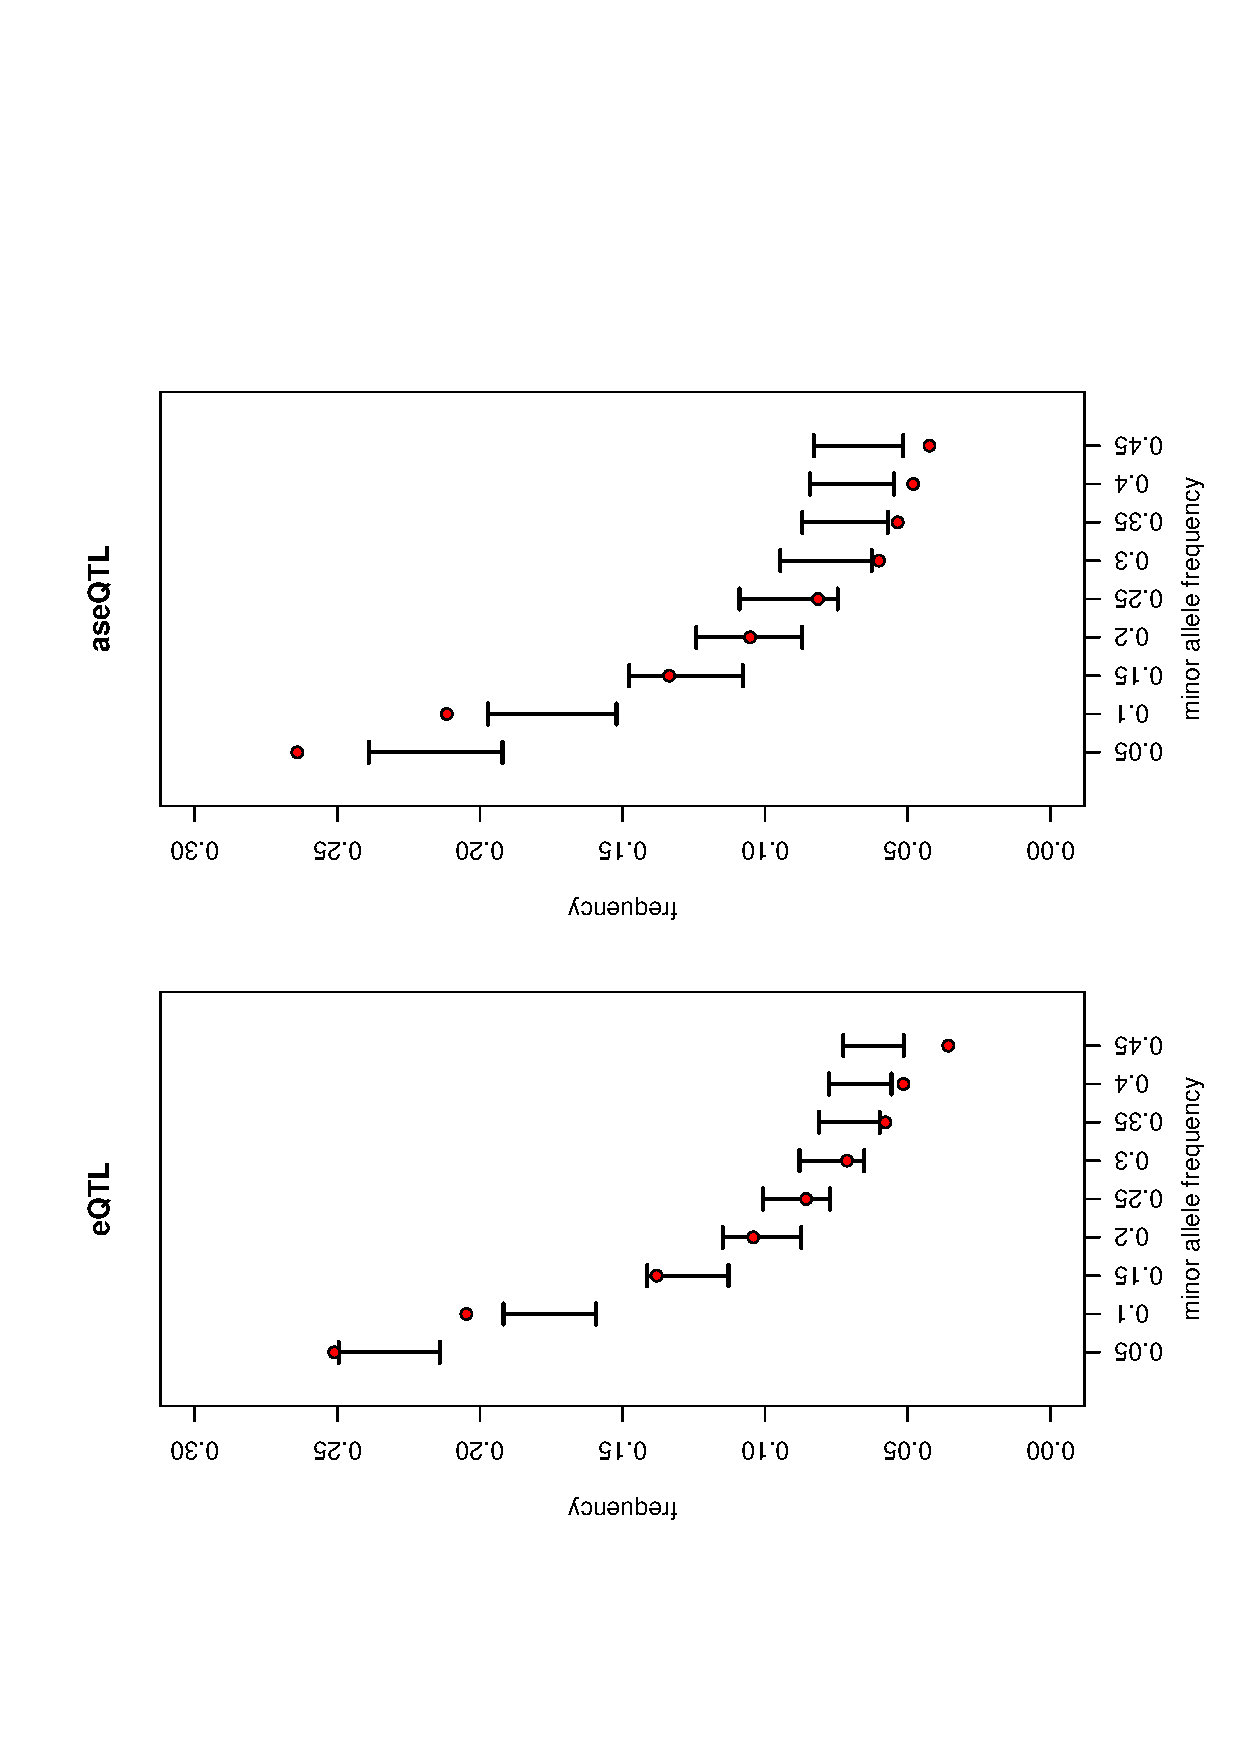
\includegraphics[width=\linewidth]{Ch3Fig3}
    \caption{\textbf{The site frequency spectra of eQTLs and aseQTLs} Minor allele frequencies of A) eQTLs and B) aseQTLs for observed data (black circles) and permuted data (gray circles, black lines are 95\% confidence intervals).}
    \label{fig:3fig3}
\end{figure}

We incorporated effect sizes to test for an additional signature of selection. Theory predicts that mutation-selection balance will maintain mutations at frequencies inversely proportional to the strength of selection acting against them \citep{Haldane1927-pj}, suggesting that QTLs under purifying selection should show a negative correlation between minor allele frequency and phenotypic effect size, assuming that phenotypic effect size correlates with the strength of selection. However, this correlation is also expected if QTLs evolve neutrally for two reasons. First, we have low power to detect rare small-effect QTLs. Second, effect size estimation error is greater for rare alleles, and when effect size is over-estimated, an association is more likely due to winner’s curse, leading to a negative correlation between effect size and minor allele frequency \citep{Capen1971-bs}. 

To avoid variation in power across allele frequency, we repeated the eQTL and aseQTL analysis, down-sampling our population to 50 individuals in each test, such that 40 individuals were drawn from the more common genotype and 10 individuals were drawn from the less common type for each SNP tested. As a consequence, for every SNP we test, sample sizes of major and minor genotype classes are equalized regardless of allele frequency in the population. We also measured effect sizes in this subsample to avoid any relationship between allele frequency and effect size estimation error. Despite reducing our sample size by half, we still detected 594 eQTLs and 670 aseQTLs, when using the most significantly associated SNP per gene (above a p-value threshold corresponding to FDR = 0.1; p \textless 2.6x10$^{-5}$ for eQTLs, p \textless 8.2x10$^{-5}$ for aseQTLs). In addition, we decoupled the identification of associations from the estimation of effect size by comparing allele frequencies of SNPs identified as eQTLs with these SNP’s effects on ASE, avoiding the double-testing issue responsible for winner’s curse.

\begin{figure}[ht!]
      \centering
       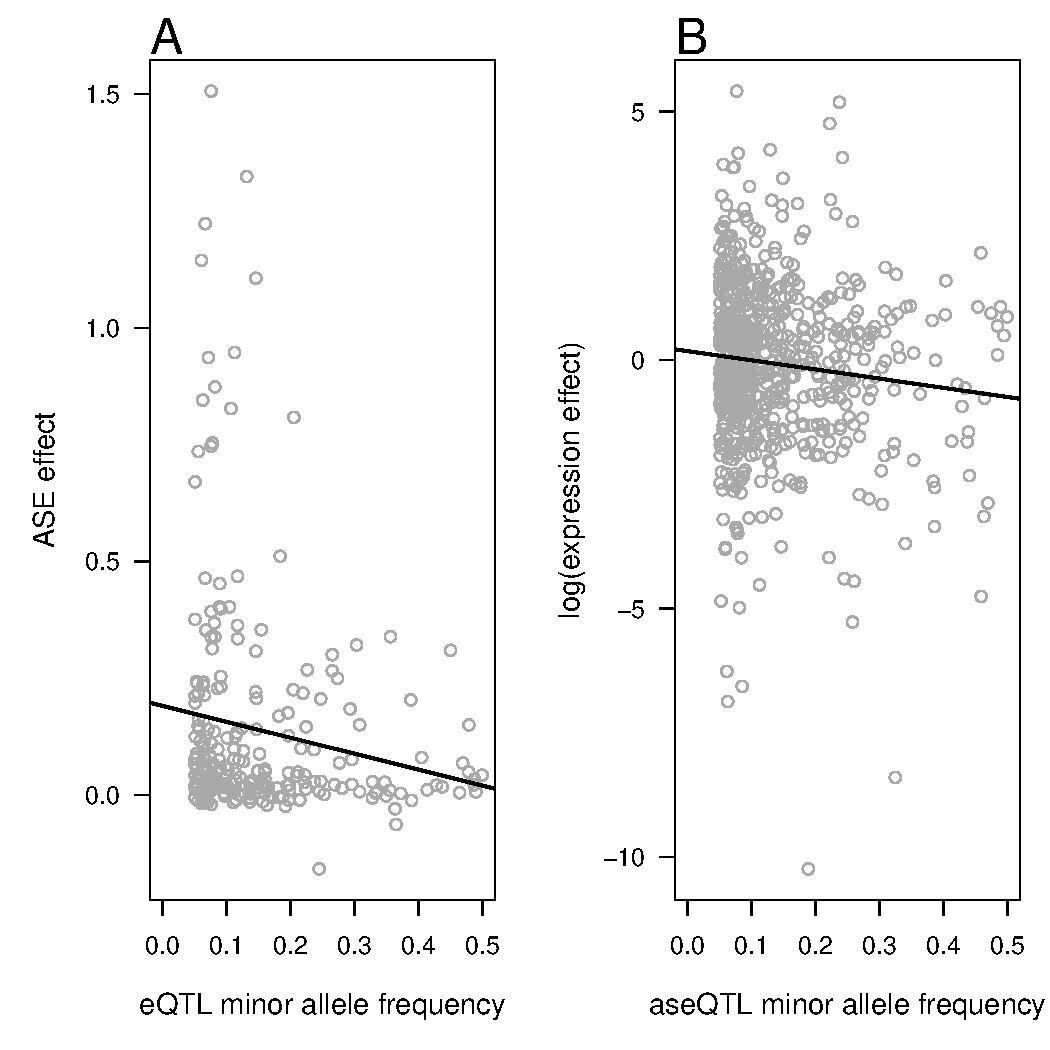
\includegraphics[width=\linewidth]{Ch3Fig4}
    \caption{\textbf{The relationship between minor allele frequency and effect size.} A) eQTL minor allele frequency is plotted against the effect of that SNP on ASE, calculated as the mean difference in ASE between individuals heterozygous at the eQTL and individuals homozygous at the eQTL. Negative values occur when the the homozygote for the eQTL has greater ASE than the heterozygote. The trend line is calculated by linear regression B) aseQTL minor allele frequency plotted against the effect of the aseQTL on total gene expression, calculated by taking the log of the absolute value of the mean difference in expression between individuals heterozygous at the aseQTL and individuals homozygous for the common allele at the aseQTL. The trend line was calculated by regression between minor allele frequency and the log of the expression effect.}
    \label{fig:3fig4}
\end{figure}

Consistent with mutation-selection balance, an eQTL’s effect on ASE was negatively correlated with eQTL allele frequency (p \textless 0.05, correlation coefficient = -0.154, n=251) and total expression effect size was negatively correlated with aseQTL allele frequency (p \textless 0.01, correlation coefficient = -0.104, n=670) (Fig.~\ref{fig:3fig4}). eQTL and aseQTL allele frequency were also negatively correlated with the corresponding effect size when we designated a random significantly-associated SNP per gene as the focal eQTL or aseQTL (Fig.~\ref{fig:3figS4} C,D). One possible explanation for the stronger association between eQTL allele frequency and ASE effect than between aseQTL allele frequency and total expression effect may be that ASE variation results from cis regulatory variation while total expression variation is determined by both cis and trans regulatory variation. Since we only map local QTLs that mainly act in cis, extra noise from trans regulatory variation likely contributes to total expression variation, weakening the association between allele frequency and total expression effect.

We also investigated the allele frequency spectra of the eQTLs and aseQTLs detected using the downsampling approach. In this case it was appropriate to use the frequencies of all SNPs tested as a neutral hypothesis because false positive and false negative rates are independent of minor allele frequency. The minor allele frequencies of the eQTLs and aseQTLs detected with downsampling were rarer than the frequencies of all SNPs tested (Fig. ~\ref{fig:3fig5}). The skew towards rare alleles was stronger here than in the QTLs detected with the whole data set, perhaps because the reduced sample size of the downsampling approach allows us only to detect large effect QTLs, which are likely to be under stronger negative selection. 

\begin{figure}[ht!]
      \centering
       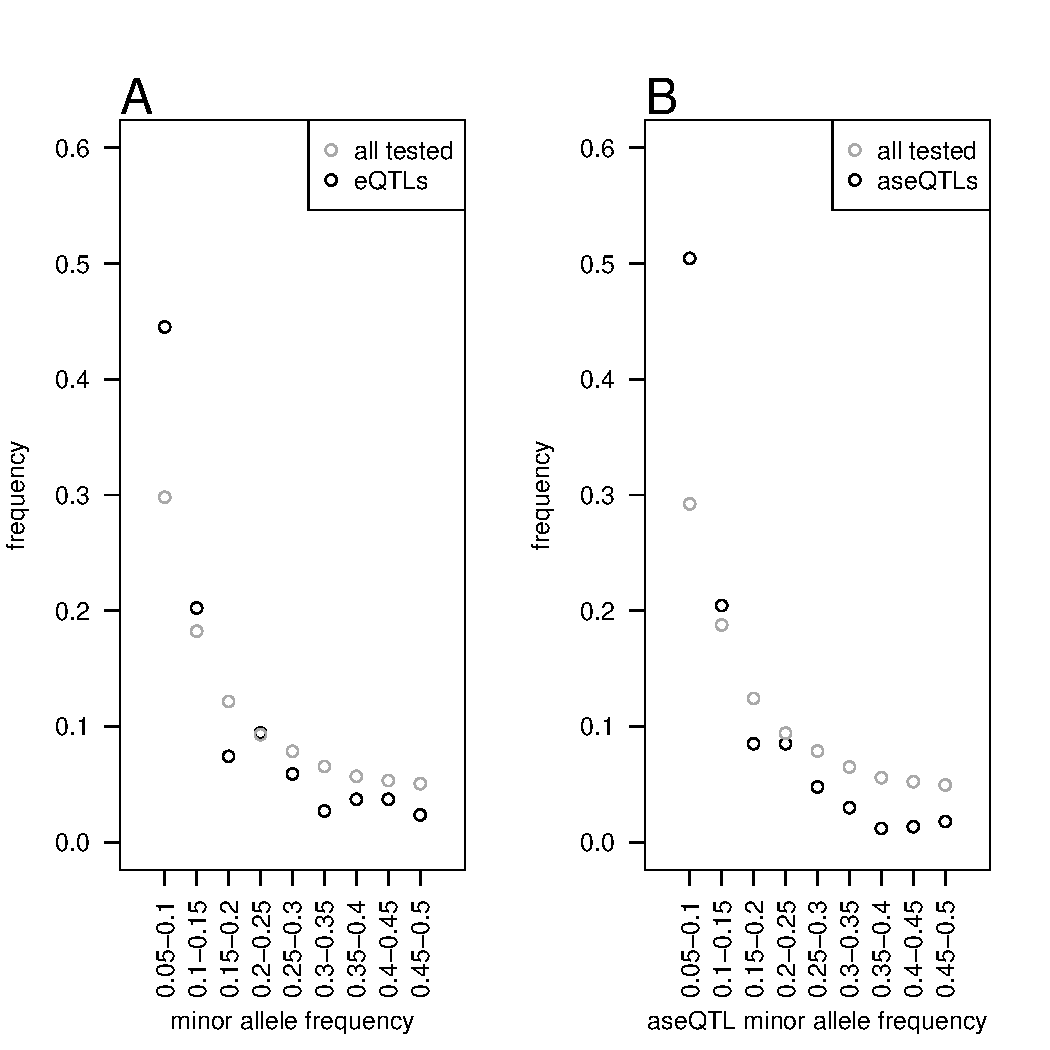
\includegraphics[width=\linewidth]{Ch3Fig5}
    \caption{\textbf{The site frequency spectra of QTLs detected in the frequency-controlled subsample.}}
    \label{fig:3fig5}
\end{figure}


It is important to note that some of our QTLs may not be causal alleles, but are instead in linkage disequilibrium with a causal allele. However, this is unlikely to strongly affect the allele frequencies of the QTLs we detect because the extent of linkage disequilibrium is constrained by similarities in allele frequency since the coefficient of linkage disequilibrium (D) is highest when the frequencies of both loci are similar. Consistent with this inference, power analyses have shown that a causal SNP and a tagging SNP in incomplete LD must have similar allele frequencies for a GWAS to successfully identify an association with the tagging SNP \citep{Zondervan2004-lo}. Therefore, our conclusions about the allele frequencies of QTLs should be robust to the inclusion of non-causal linked alleles. 

Our mapping of QTLs for expression and allele-specific expression genome-wide in a single population of \textit{C. grandiflora} demonstrates that the frequencies and phenotypic effect sizes of these QTLs are consistent with mutation-selection balance. In addition, the enrichment of eQTLs in CNSs directly upstream of genes further supports CNS’s potential role as regulatory elements; however, the large number of QTLs discovered outside of conserved regions suggests significant turnover in regulatory elements between species. Alternatively, QTLs may create new deleterious regulatory interactions, instead of disrupting conserved functional sites. Taken together, our results, indicate that much of local expression variation observed at the population level is deleterious and support the role of mutation-selection balance in maintaining genetic variation within populations.

\section{Materials and Methods}

\subsection{Study system and plant material}
\textit{Capsella grandiflora} is an obligately outcrossing member of the Brassicaceae family with a large effective population size ($N_{e} \sim$ 600,000), relatively low population structure and a range that spans northern Greece and southern Albania \citep{Slotte2010-gw,St_onge2011-jz}. In June 2010, we collected seeds from approximately 400 plants growing in a roadside population of \textit{C. grandiflora} near Monodendri, Greece (Population Cg-9(30)). We germinated and grew one individual from each parent in the University of Toronto greenhouses and performed crosses between independent random pairs of plants to generate the seeds used in this study. By growing the parents in a common environment and then assaying their progeny in a common environment, we reduced the influence of maternal effects and unknown micro-environmental effects on gene expression.

Approximately 10 seeds from each cross were sterilized in 10\% bleach followed by 70\% ethanol, placed on sterile plates filled with 0.8\% agar with Mursashige-Skoog salts (2.15 g/L), stratified in the dark at 4$^{o}$C for one week, and then allowed to germinate in a growth chamber at 22$^{o}$C and 16 hour photoperiod. After one week, we transplanted two of the seedlings from each cross into 4 inch pots filled with ProMix BX soil and returned the pots to the growth chamber. After another week, pots were thinned down to one seed per cross. Throughout the experiment, pots were randomized once every week to minimize location effects.

Leaf tissue from young leaves was collected for RNA extraction four weeks after transplanting and immediately flash frozen in liquid nitrogen. RNA was extracted using plant RNA extraction kits (Sigma) from 2 or 3 samples from each plant. The extracted RNA was quantified with a Qubit spectrophotometer and the samples from each plant were pooled such that each pool contained the same amount of RNA from each sample. RNA was sequenced at the Genome Quebec Innovation Centre on two flow cells with 8 samples per lane. Reads were 100bp long and paired end. We extracted DNA from leaf tissue using a CTAB based protocol. Whole genome sequence from each individual was obtained through 100 cycles of paired-end sequencing in a Hiseq 2000 with Truseq libraries (Illumina), with three individuals sequenced per lane.

\subsection{Genomic data}
We mapped DNA sequence data to the \textit{C. rubella} reference genome \citep{Slotte2013-py} with Stampy v1.0.19 \citep{Lunter2011-uc}. After bioinformatic processing with Picard tools, we realigned reads around putative indels with GATK RealignerTargetCreator and IndelRealigner and compressed the resulting bams with GATK ReduceReads \citep{DePristo2011-jc}. Raw SNP calls were generated by joint calling of all samples in GATK v2.81 UnifiedGenotyper. We subsequently followed GATK Best Practices for Variant Quality Recalibration using a high confidence subset of the  raw calls generated by filtering snps for concordance with common variants (minor allele frequency \textgreater 0.11) in a species-wide sample of \textit{C. grandiflora} \citep{Williamson2014-tf} as well as suspect realignments (transposable elements, centromeres, 600bp intervals containing extreme Hardy-Weinberg deviations, 1kb intervals with evidence of 3 or more snps in reference-to-reference mapping). A relatedness analysis revealed that six individuals were more related to eachother than expected in an outcrossing population, perhaps because of introgression from \textit{C. rubella}, so we removed these individuals from the analysis. We measured population structure using fastStructure on a set of 56,011 biallelic snps distributed genome wide that had been pruned for LD following the recommended analysis stream \citep{Raj2014-im}.

To map RNA reads, we constructed our own codon-only reference sequence by stitching together the exons and UTRs of each gene into a scaffold using reference gene annotations \citep{Slotte2013-py}. We mapped to this codon-only reference using Stampy 1.0.21 with default settings \citep{Lunter2011-uc}. We chose to use Stampy over other RNA-specific aligners, like Tophat, because visual examination of alignments showed that Stampy was better at mapping reads containing multiple polymorphisms, reducing the potential for false associations between expression level and the genotypic variants that affect mapping (Fig.~\ref{fig:3figS6}). RNAseq readmapping for two individuals was very poor quality (\textless10\% reads mapped and paired correctly), so these individuals were removed. Our final sample size was 99 individuals.

Expression level was measured with the HTSeq.scripts.count feature of HTSeq, which counts the number of read pairs that map to each gene \citep{Anders2015-qa}. We normalized the read counts of each sample for library size by dividing read counts by the median read count of the entire sample. Previous studies on human gene expression have found interactions between GC content, lane, and expression level (12), but we did not detect this (Fig.~\ref{fig:3figS7}). Genes with a median expression level below five reads per individual before normalization were removed from the analysis, leaving a total of 18,692 genes.

\subsection{Mapping local eQTL}
We selected SNPs for our eQTL analysis by finding all SNPs within the window spanning 5 kb upstream of the gene’s transcription start site and 5kb downstream from the gene’s transcription end site. We chose the 5kb range because a previous study in \textit{Arabidopsis thaliana} mapping associations between expression and SNPs within 30kb of the gene found that 87\% of local eQTLs were located within 5kb of the gene \citep{Gan2011-xv}. SNPs were categorized as occurring in 0-fold degenerate sites, 4-fold degenerate sites, 2 or 3-fold degenerate sites, 5\textsc{\char13}UTRs, 3\textsc{\char13}UTRs, introns, stop codons, or intergenic regions based reference annotations\citep{Slotte2013-py}. In addition, we identified SNPs located in non-coding sequence conserved across the Brassicaceae family \citep{Haudry2013-qe}. We only included SNPs with at least 10 heterozygous individuals and 10 individuals that were homozygous for the common allele in our sample.

We wrote set of Python scripts to test for associations between expression level and genotype at a nearby SNP. These scripts are available at https://github.com/emjosephs/eQTL. We mapped eQTLs by conducting a Mann-Whitney U test on the null hypothesis that gene expression does not differ between individuals that were homozygous for the common allele and individuals that were heterozygous. We used non-parametric statistics because expression data is not normally distributed. We used the Mann-Whitney U test function in SciPy (“scipy.stats.mannwhitneyu”) \citep{Jones2001-in}, which uses a continuity correction and corrects for ties. 8,302 of our genes had ties in expression level between individuals and these ties on average involved 4.5 individuals. In addition,we compared common homozygotes to heterozygotes because we expect most local eQTLs to act in cis and thus be additive \citep{Pickrell2010-ci}, and because not being limited by the sample size of rare homozygotes allowed us to map eQTL at rarer alleles. 

To avoid a relationship between allele frequency and sample size, we conducted a second eQTL analysis where we randomly subsampled 50 individuals for each SNP tested so that 40 individuals had the most common genotypic category (usually the homozygote) and 10 had the less common genotypic category (usually heterozygote) \citep{Battle2014-ke}. We chose these thresholds because they retained most individuals while allowing us to still test 3,972,771 of the 4,098,832 SNPs originally tested for eQTLs (96.9\%).

For both eQTL analyses, we controlled for multiple testing by using a false discovery rate approach \citep{Storey} and only considered eQTLs to be associated with expression if that association had a p value corresponding to a false discovery rate of 0.1. To avoid being biased by detecting multiple SNPs linked to only one causal site, we only selected one eQTL per gene, picking the SNP with the lowest p value for association. However, to investigate whether choosing the most associated SNP biased our results, we also performed all analyses with eQTLs that were randomly chosen from the pool of SNPs significantly associated with expression (FDR = 0.1). We calculated the expression effect size of eQTLs by taking the absolute value of the difference between mean expression in the common homozygote and mean expression in the heterozygote. 

\subsection{Mapping aseQTL}
If local eQTLs act in cis, they should have allele-specific effects and individuals heterozygous for an eQTL will show a larger difference in expression between alleles than individuals homozygous for an eQTL. To take advantage of this second signature of expression variation, we developed a method to test for allele-specific expression QTL, or ‘aseQTL’ (similar approaches have been used in humans in \citet{Battle2014-ke}). We quantified allele-specific expression at all heterozygous sites inferred from the genomic data. We used the count of reads mapped to each allele, taken from the ‘AD’ values in a VCF file constructed from the RNAseq data using GATK Unified Genotyper to calculate an allele-specific-expression measure (‘ASE) for each gene in each individual. Specifically, we calculated the mean of the the differences in allelic expression values at all heterozygous sites across a gene and divided this mean by median expression level of all genes in the individual to control for sequencing depth. While we expected that our measure of gene-wide ASE would be more accurate when we required multiple heterozygous sites per gene, doing so did not strongly alter the number of aseQTLs we found or their allele frequency distribution, so we only required one heterozygous site per gene to measure ASE (Fig.~\ref{fig:3figS8}).

ASE measures were not normally distributed, so we used a Mann-Whitney U test to test the null hypothesis that ASE did not differ between individuals that were heterozygous at a given SNP and individuals that were homozygous for either allele at that SNP. As before, we used the mannwhitneyu function in the SciPy package. 8,334 genes had at least one tie between individuals for ASE value and an average of 4 individuals were involved in ties within these genes. We only tested SNPs where we had 10 individuals that were both heterozygous at the SNP and had a heterozygous marker site in the gene and 10 individuals that were homozygous at the SNP and had a heterozygous marker site in the gene, allowing us to test for associations at 17,880 genes. We designated aseQTLs as the most associated SNP per gene that had higher ASE in heterozygotes for that SNP than in homozygotes for that SNP. However, we also performed all analyses designating aseQTLS as a SNP that was randomly sampled from the set of SNPs that were significantly associated with expression (FDR = 0.1) and had greater ASE in homozygotes for that SNP than heterozygotes.

As in the eQTL analysis, we conducted a second aseQTL analysis where we subsampled 50 individuals for each SNP tested such that 40 had the most common genotypic category (usually the homozygote) and 10 had the less common genotypic category (usually heterozygote). This sample size allowed us to test 3,841,452 of the 3,966,364 SNPs originally tested for aseQTL (96.8\%). For both sets of analyses, we conducted a false discovery rate analysis as described in the eQTL section and, selected all SNPS with a p value below the FDR threshold of 0.1, we chose the most significantly associated SNP per gene for further analysis, with the additional requirement that heterozygous individuals have higher ASE than homozygous individuals. We calculated ASE effect size for aseQTLs and eQTLs by taking the difference between mean ASE in homozygotes and mean ASE in heterozygotes. We only report ASE effects for eQTLs located outside the coding sequence of these genes they regulate.

Preferential mapping of reference alleles compared to alternative alleles could lead to spurious ASE. To evaluate the importance of this effect, we simulated all of the possible reads spanning each heterozygous site, containing either the reference allele or an alternate allele using scripts from \citep{Degner2009-nj}. There were up to 200 reads possible for each site, although reads near the start and end of genes had fewer reads covering them since we discarded all reads that were less than 100bp long. We mapped these reads with the same program and settings we used for the real data, with the exception that these reads were single-ended.  Out of 2,365,590 SNPs in coding regions, 19,017 SNPs (\textless1\%) had unequal numbers of reads mapping from each allele. 11,339 (60\%) of these sites had more reads that mapped with the reference allele than with the alternative allele, suggesting that there is some reference bias. The 19,017 SNPs with evidence of mapping bias occurred in 3,059 genes. Removing these genes from the analysis did not qualitatively affect the minor allele frequency of aseQTLs (Fig.~\ref{fig:3figS9})

\subsection{Permutation analysis}
Conducting millions of tests for genotype-expression associations with a relatively small (n=99) sample size exposes us to two potential sources of bias that correlate with the allele frequency of the SNPs we are testing. First, smaller sample sizes at low frequencies reduce power to detect associations. Second, smaller sample sizes at low frequencies increase our risk of false positives because expression data is non-normally distributed and outliers in a small sample will have a disproportionate effect on the mean. We found this second possibility especially concerning because it is not conservative with respect to our hypothesis that purifying selection will maintain eQTLs and aseQTLs at lower allele frequencies. 

To ensure that our conclusions about allele frequencies were not due to false positives being more common at low allele frequencies, we compared the eQTLs and aseQTLs we found with those discovered using permuted data. We constructed permutations by randomly shuffling the assignments between genotype and expression values or allele-specific expression values for each gene. This strategy allows us to retain the allele frequencies and spatial distributions of the SNPs we are testing along with the distribution of expression and allele-specific expression values of each gene. Each permuted set was analyzed using the same methods as the real data, with one exception: instead of calculating a FDR for each permuted data set, we used the p-value cut offs from the real data to identify ‘false-positive’ eQTLs and aseQTLs in the permuted data. The frequency distributions of these ‘false-positive’ QTLs were used as a null distribution for the expected frequency of QTLs.

The permutation analyses do not directly control for site type, recombination rate, or other factors that could both bias a SNP towards being an eQTL/aseQTL and reduce allele frequency. To ensure that these effects did not drive our observations, we divided our eQTLs and aseQTLs from the real data and from permuted data into subsets. First, for site type, we selected the most strongly associated eQTL and aseQTL per gene that came from a the site-type of interest. Our site types were 5’UTRs, 3’UTRs, introns, intronic CNSs, exons (divided into 5 regions based on distance from start and end of the gene), and upstream and downstream CNS and nonconserved regions. For upstream and downstream regions, we divided sites into those within 1 kb of the TSS/TES and those that were 1 to 5 kb from the TSS/TES. 

To control for recombination rate, we divided SNPs into those coming from high recombination regions (> 3.45 cM/mB) and low recombination regions (< 3.45 cM/mB) using recombination rate data calculated by using a genetic map made from a cross between \textit{C. rubella} and \textit{C. grandiflora} \citep{Corbett-Detig2015-yo}. To test for confounding effects due to gene conversion, we divided SNPs into those whose mutations could be due to gene conversion (A or T and C or G) and others (A and T or G and C).

\section{Acknowledgements}
We thank Niroshini Epitawalage, Amanda Gorton, and Khaled Hazzouri for lab assistance, J. Paul Foxe for collection assistance, Wei Wang for computer assistance, and Aneil Agrawal, Graham Coop, Asher Cutter, Alan Moses, Adrian Platts, Tanja Slotte, and Robert Williamson for helpful suggestions. Thomas Bureau, Mathieu Blanchette, Daniel Schoen, Paul Harrison, Alan Moses, Adrian Platts, and Eef Harmsen contributed to the Value-directed Evolutionary Genomics Initiative (VEGI) grant (Genome Quebec/Genome Canada) which supported this work, along with an NSF Graduate Research Fellowship to EBJ (DGE-1048376), and NSERC Canada and CFI grants to JRS and SIW. 

\section{Appendix: Supplementary figures}

\begin{figure}[ht]
      \centering
       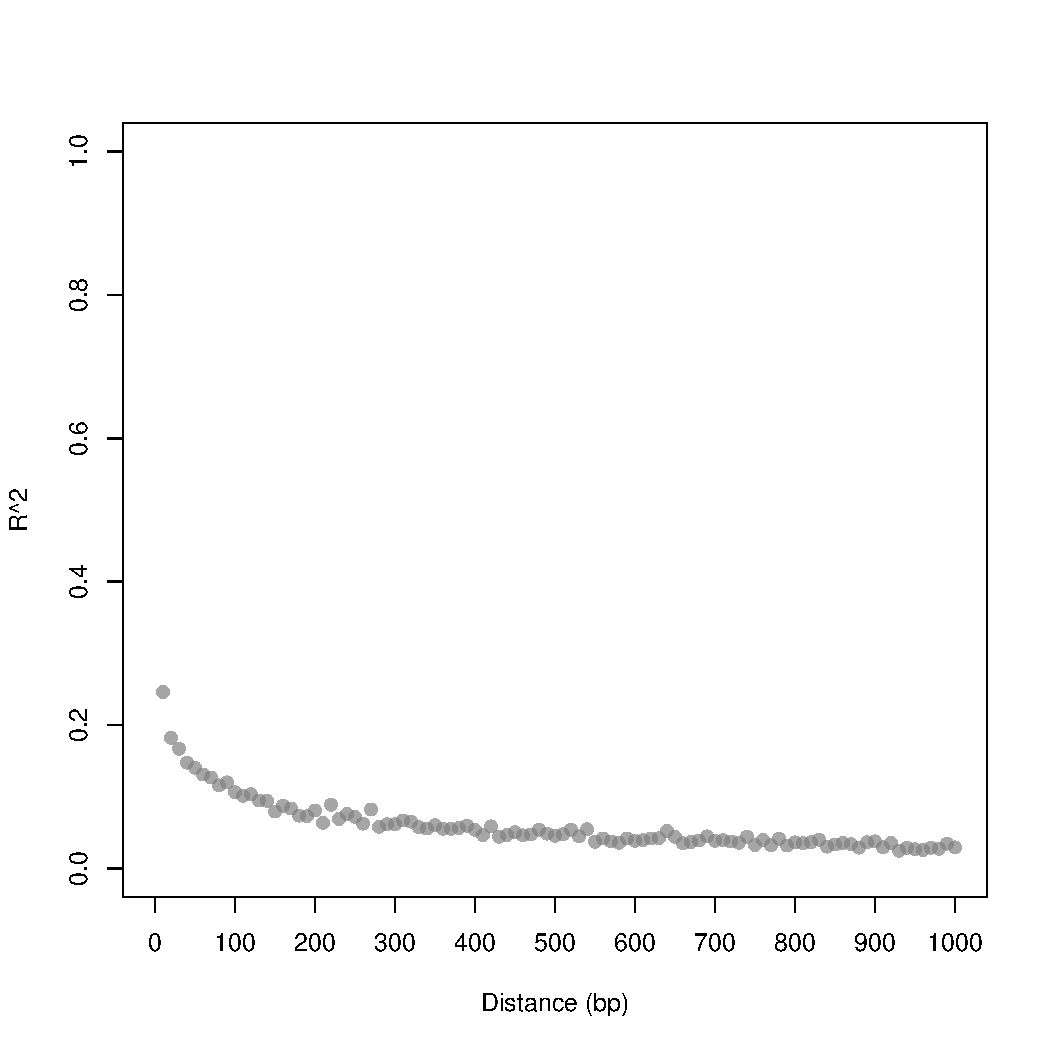
\includegraphics[width=\linewidth]{Ch3FigS1}
    \caption{\textbf{Linkage disequilibrium in \textit{C. grandiflora}.} Linkage disequilibrium was calculated for all SNPs within 1kb of each other on scaffold 2. 1\% of these pairs were randomly sampled for the above figure, which shows mean $r{^2}$ between pairs in 10bp bins.}
    \label{fig:3figS1}
\end{figure}

\begin{figure}[ht]
      \centering
       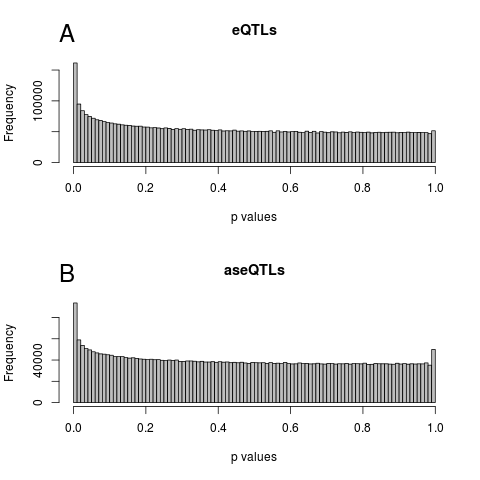
\includegraphics[width=\linewidth]{Ch3FigS2}
    \caption{\textbf{The distribution of p values for all SNPs tested in A) eQTL analyses and B) aseQTL analyses}}
    \label{fig:3figS2}
\end{figure}

\begin{figure}[ht]
      \centering
       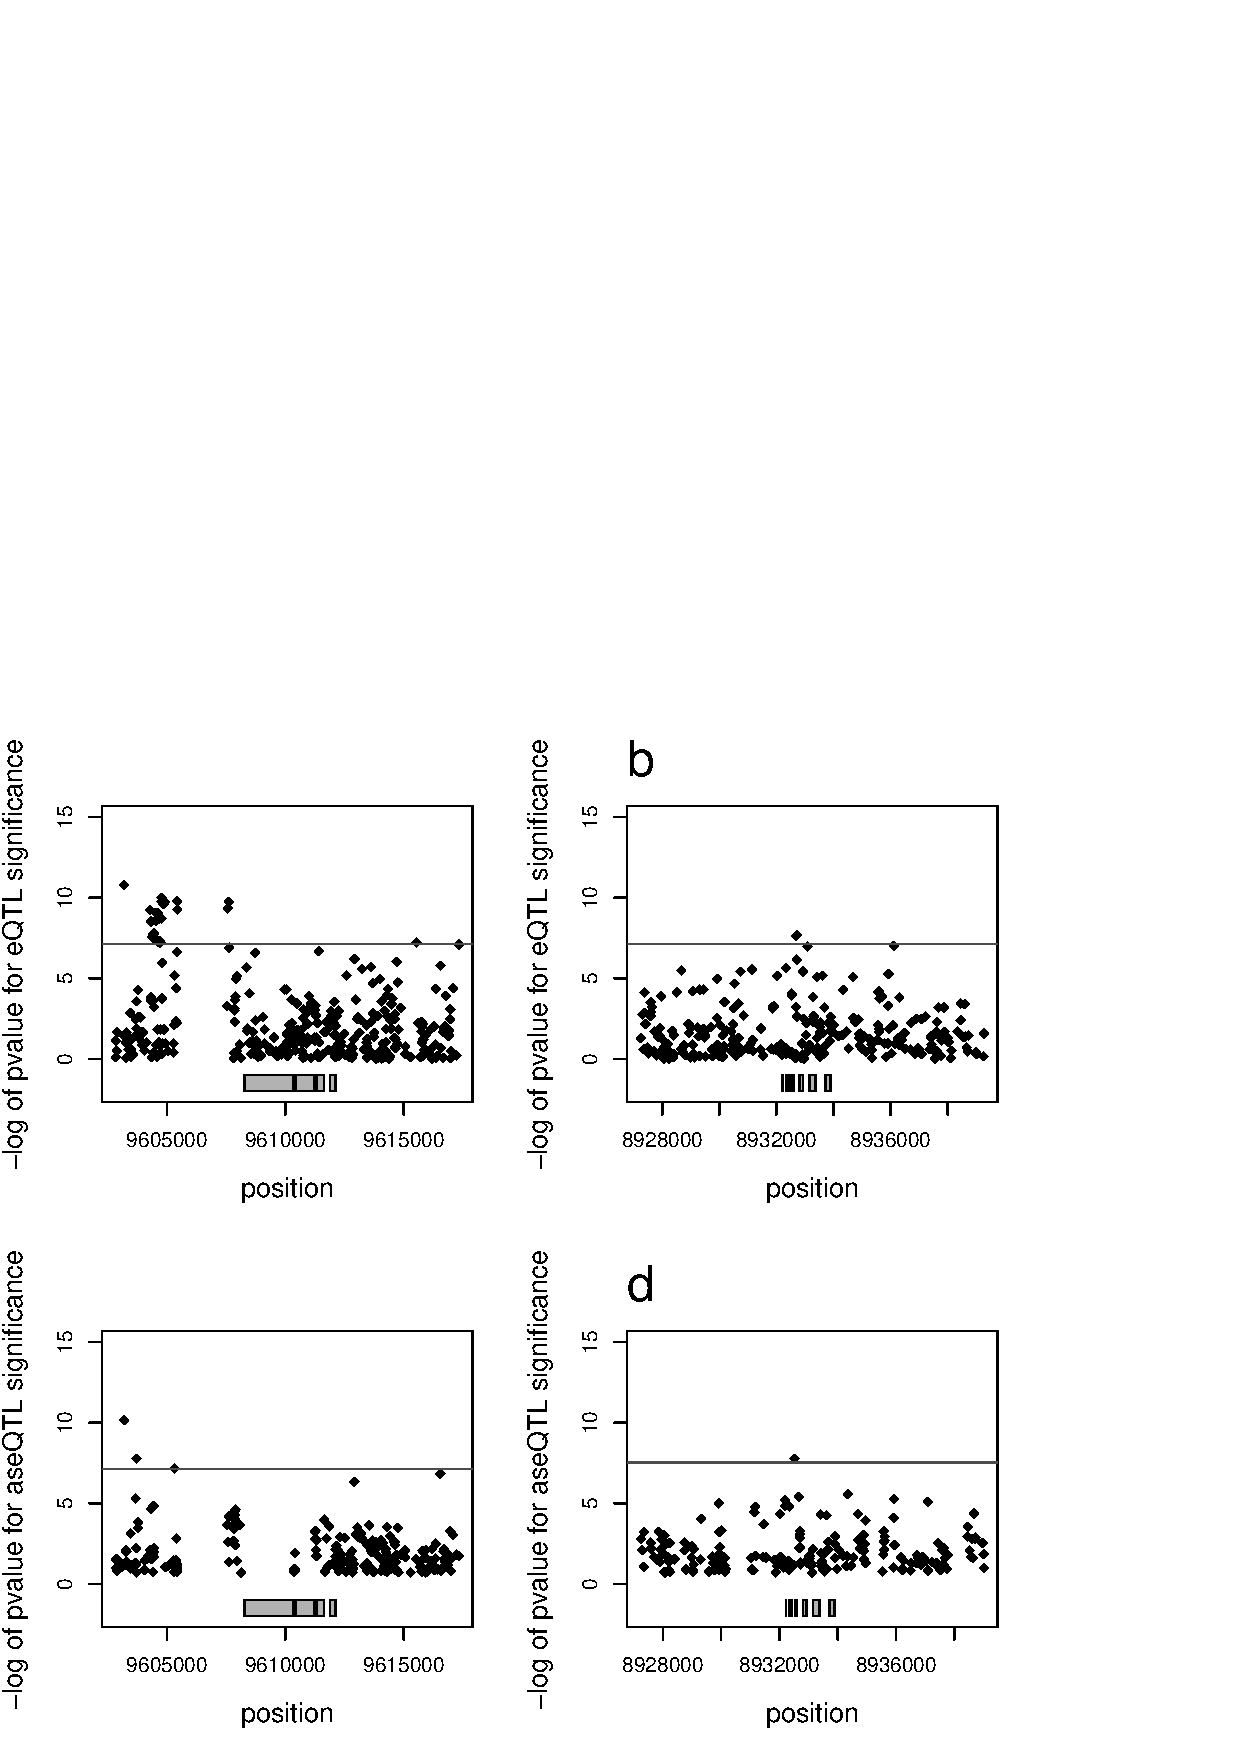
\includegraphics[width=\linewidth]{Ch3Examples}
    \caption{\textbf{Example eQTL and aseQTL genes.} Manhattan plots for associations between SNPs and total expression (A and B) and ASE (C and D) for two genes, PAC:20895445 (A and C) and PAC:20904926 (B and D). Each black dot represents a SNP and is plotted by genomic position on the x axis and the negative log of the p value for association on the y axis. The gray line denotes the p value threshold corresponding to an FDR of 0.01. The gray boxes represent the exons of the gene. Note that PAC:20895445 is an ortholog of AT4G16250.1, PHYTOCHROME D and PAC:20904926 is an ortholog of ATG68185.1, a ubiquitin-like superfamily protein.}
    \label{fig:3figS3}
\end{figure}

\begin{figure}[ht]
      \centering
       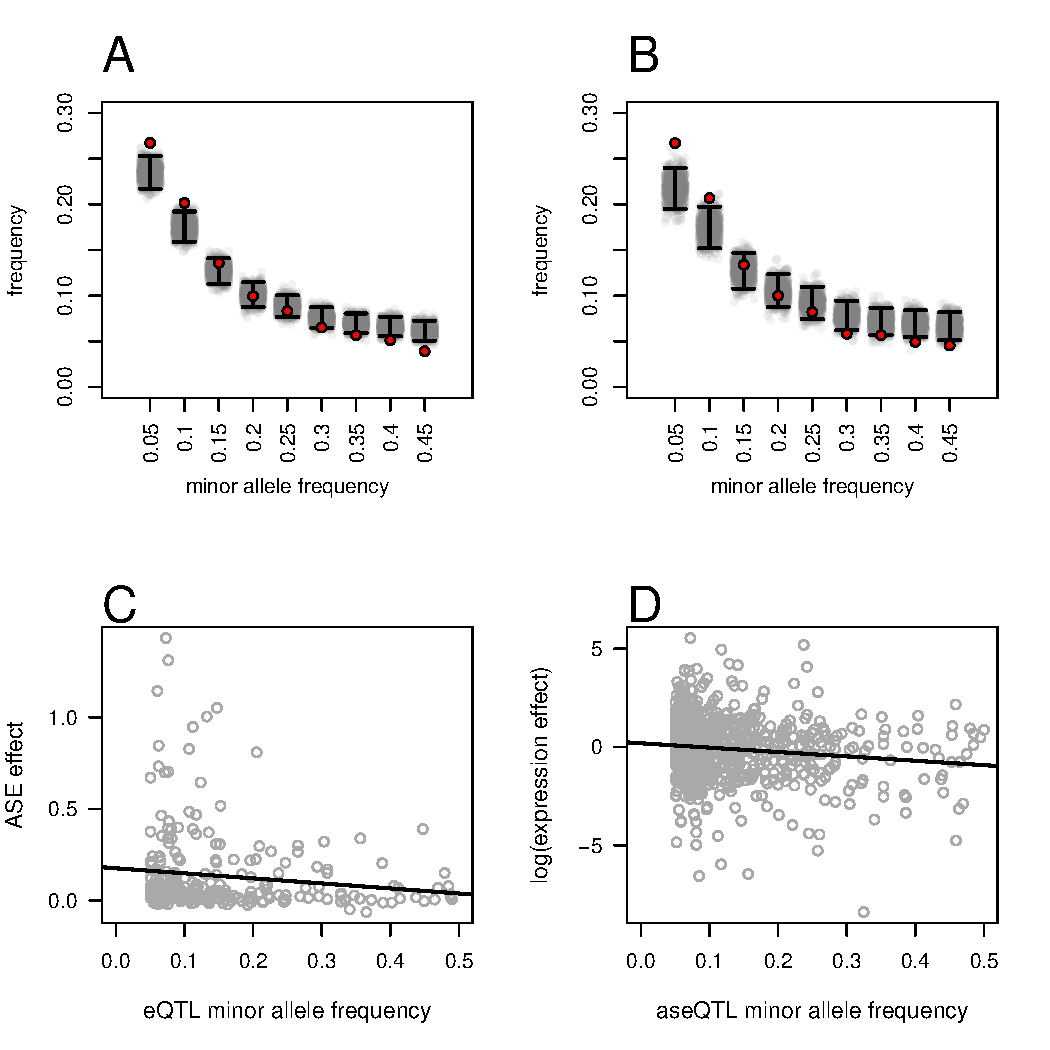
\includegraphics[width=\linewidth]{Ch3FigS4}
    \caption{\textbf{The effect of designating a random associated SNP per gene as eQTL/aseQTL instead of the most associated SNP per gene.} The site frequency spectrum of A) eQTLs and B) aseQTLs for observed data (red circles) and permuted data (gray circles, black lines are 95\% confidence intervals) when a random SNP is chosen per gene to be an eQTL or aseQTL. The same eQTLs and aseQTLs are plotted in C) and D). In C), eQTL minor allele frequency is plotted against the effect of that SNP on ASE, calculated as the mean difference in ASE between individuals heterozygous at the eQTL and individuals homozygous at the eQTL. Negative values occur when the the homozygote for the eQTL has greater ASE than the heterozygote. The black line is calculated by linear regression. In D), aseQTL minor allele frequency plotted against the effect of the aseQTL on total gene expression, calculated by taking the log of the absolute value of the mean difference in expression between individuals heterozygous at the aseQTL and individuals homozygous for the common allele at the aseQTL. The trend line was calculated by regression between minor allele frequency and the log of the expression effect. }
    \label{fig:3figS4}
\end{figure}

\begin{figure}[ht]
      \centering
       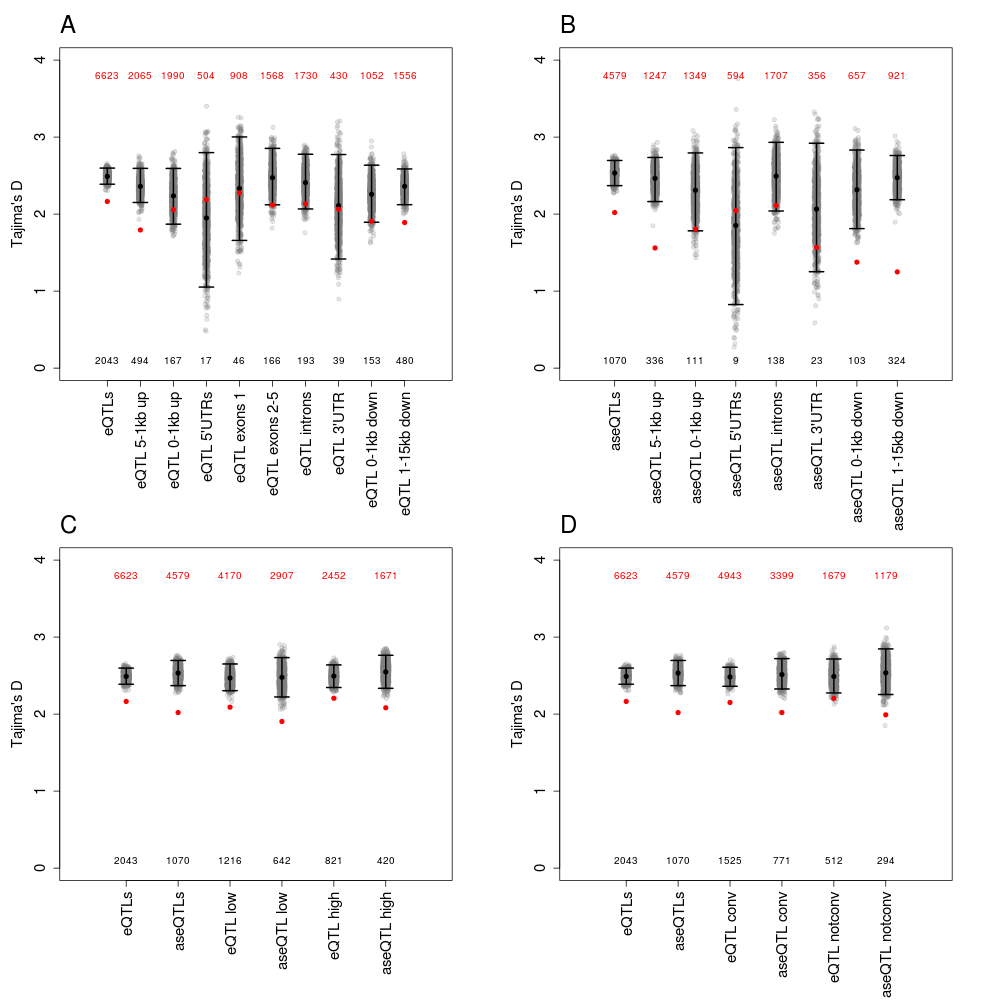
\includegraphics[width=\linewidth]{Ch3FigS5}
    \caption{\textbf{Tajima\textsc{\char13}s D of eQTLs and aseQTLs within site type, recombination rate, and substitution type.} A) Tajima\textsc{\char13}s D for eQTLs of various categories. Red circles are the real data, gray circles show Tajima\textsc{\char13}s D for permuted eQTLs, and black lines show 95\% confidence intervals. Tajima\textsc{\char13}s D was used to summarize the site frequency spectra and make plots more readable than they would be if raw frequencies were plotted. The total number of eQTLs in each category is shown with the red numbers and the mean number of permuted eQTLs in each category is shown with the black numbers. B) The same data as A) but for aseQTLs. C) Tajima\textsc{\char13}s D for eQTLs and aseQTLs (red dots) and permuted eQTLs and aseQTLs (gray dots, black bars are 95\% confidence intervals) for sites in low recombination regions (\textless 3.45 cM/mB) and high recombination regions (\textgreater 3.45 cM/mB). D) Tajima\textsc{\char13}s D for A/T to G/C substitutions that could be favored by gene conversion (‘conv’) and other substitutions (‘notconv’). Note that all Tajima\textsc{\char13}s D values are significantly increased because only SNPS above a certain allele frequency were testable, so that even for 4\-fold degenerate sites in the analysis, Tajima\textsc{\char13}s D is 2.403.}
    \label{fig:3figS5}
\end{figure}

\begin{figure}[ht]
      \centering
       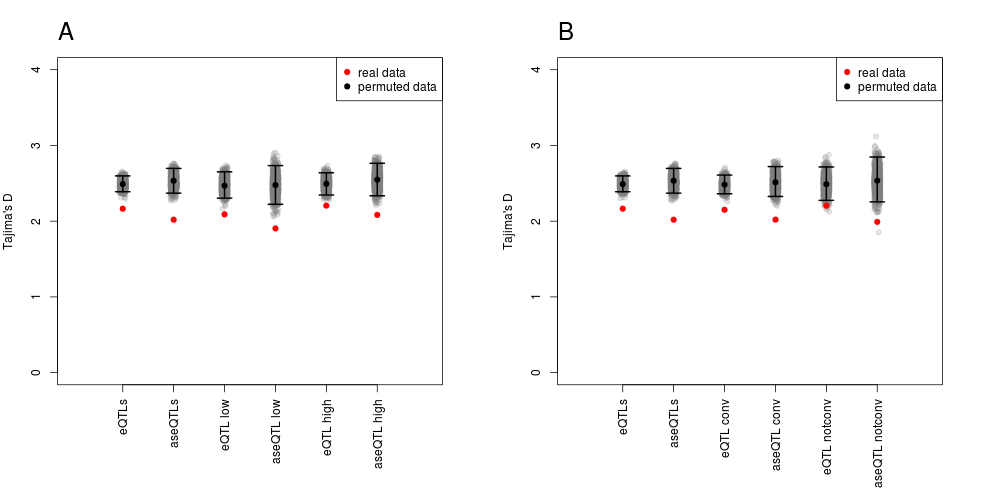
\includegraphics[width=\linewidth]{Ch3FigS6}
    \caption{\textbf{A comparison of mapping programs in highly polymorphic regions.} RNAseq coverage for an example gene using mapping from Tophat (top) and Stampy (bottom). Colored lines indicate polymorphic sites compared to the reference. The arrows indicate regions where coverage was reduced in Tophat because of multiple polymorphisms. Note that Tophat reads have splice junctions while Stampy reads do not because we mapped to an exon-only reference.}
    \label{fig:3figS6}
\end{figure}

\begin{figure}[ht]
      \centering
       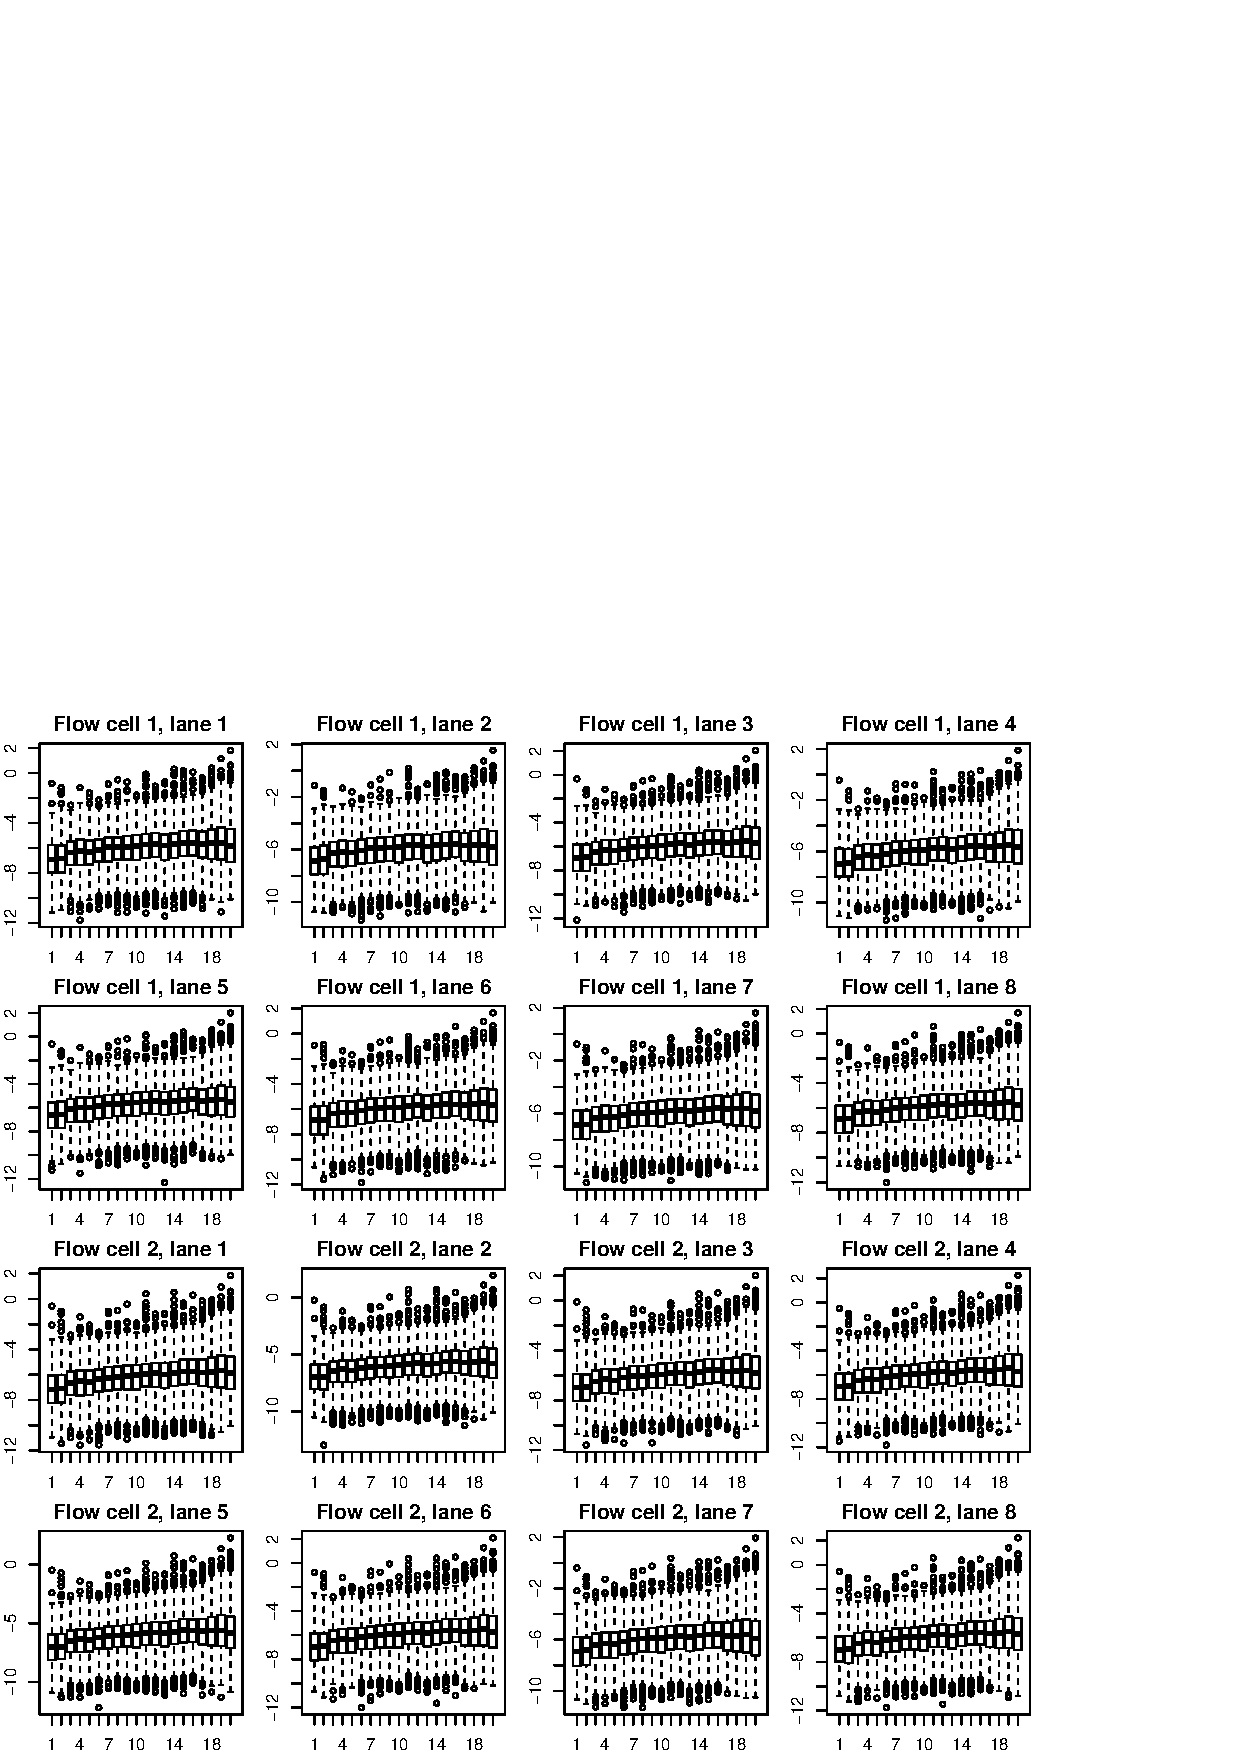
\includegraphics[width=\linewidth]{Ch3FigS7}
    \caption{\textbf{GC composition and expression by lane.} All genes included in the study were split into 20 equally sized bins by GC content. Expression in these bins was combined for each lane and plotted in box plots.}
    \label{fig:3figS7}
\end{figure}

\begin{figure}[ht]
      \centering
       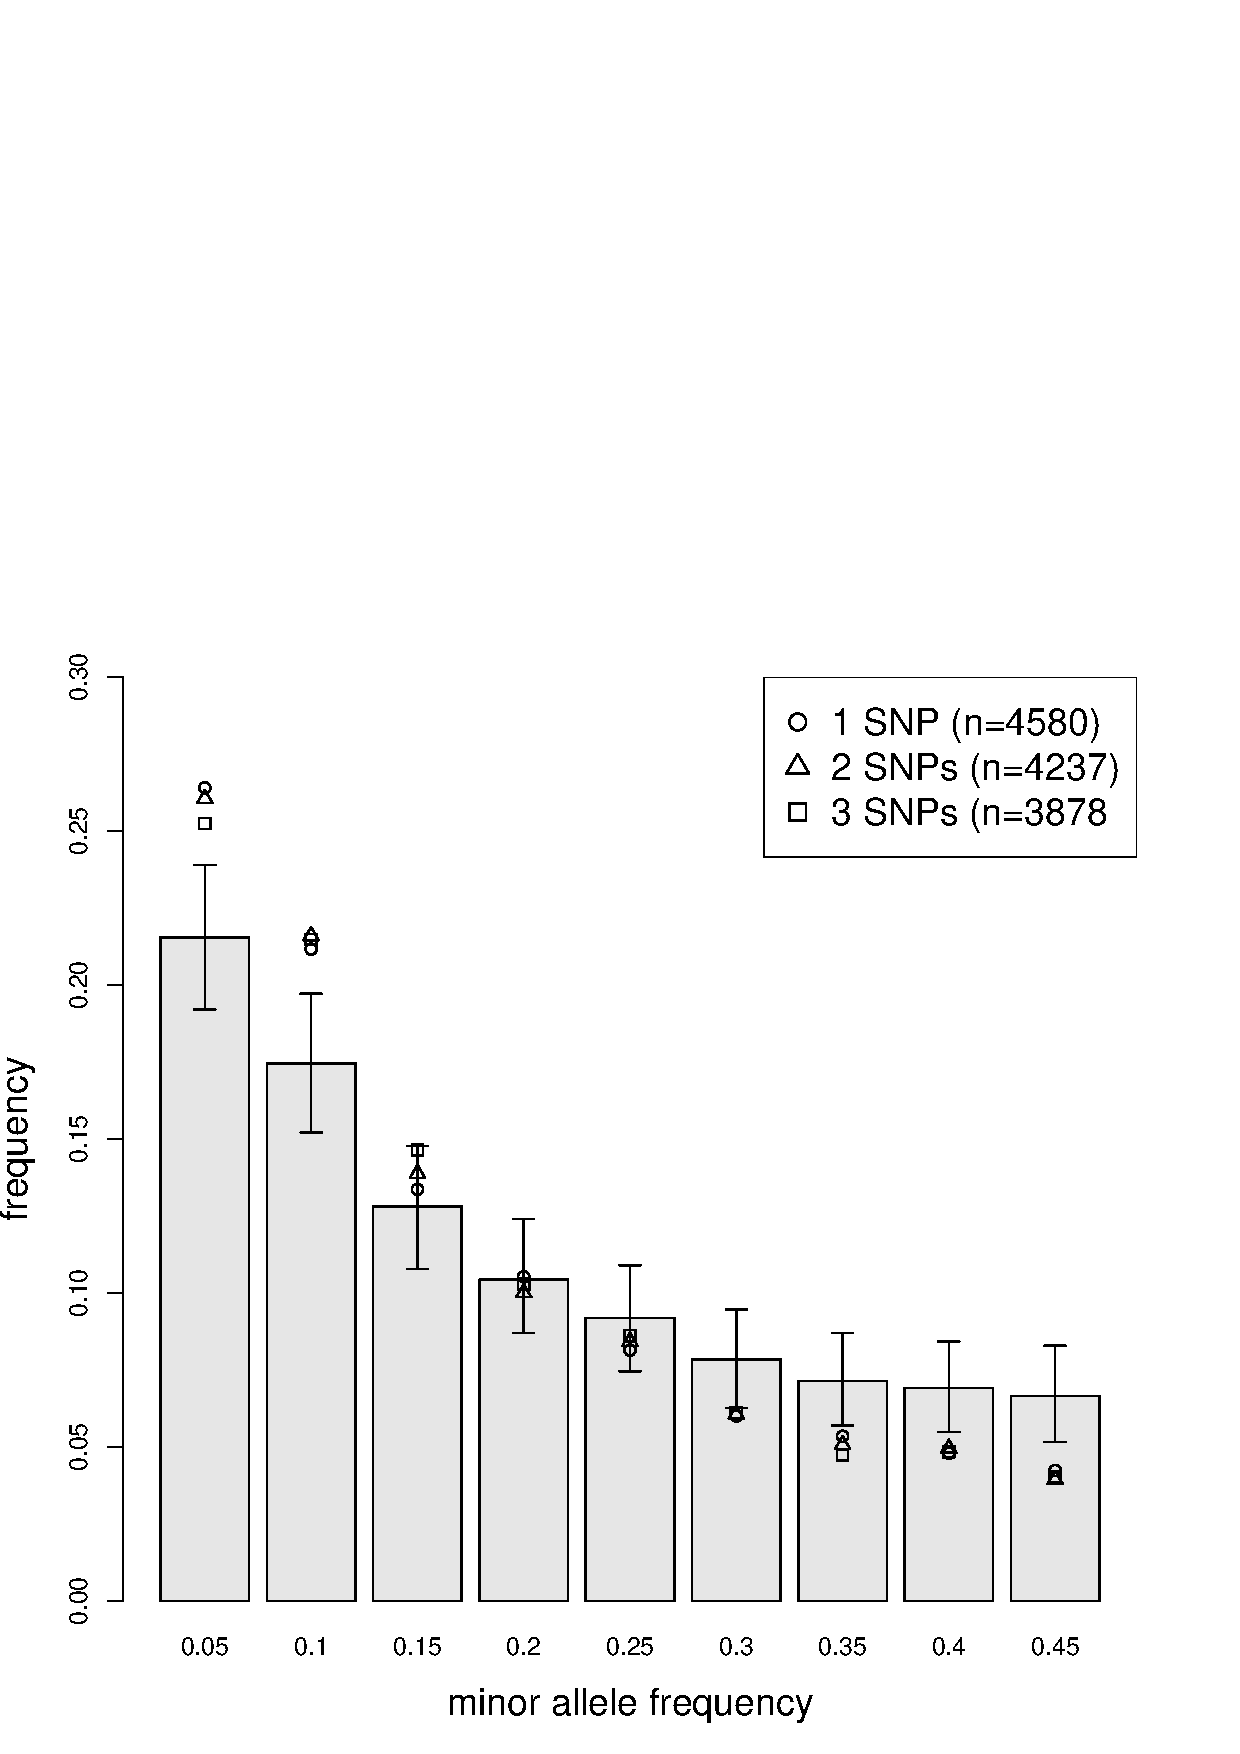
\includegraphics[width=\linewidth]{Ch3FigS8}
    \caption{\textbf{The effect of increasing the number of SNPs required to measure ASE effects aseQTL detection.} The minor allele frequency of aseQTLs detected when ASE measurement required 1 heterozygous coding SNP (circles), 2 SNPs (triangles), and 3 SNPs (squares). While increasing the numbers of SNPs required to measure ASE reduced the number of aseQTLs detected, it did not qualitatively change our conclusions about the rareness of aseQTLs.}
    \label{fig:3figS8}
\end{figure}

\begin{figure}[ht]
      \centering
       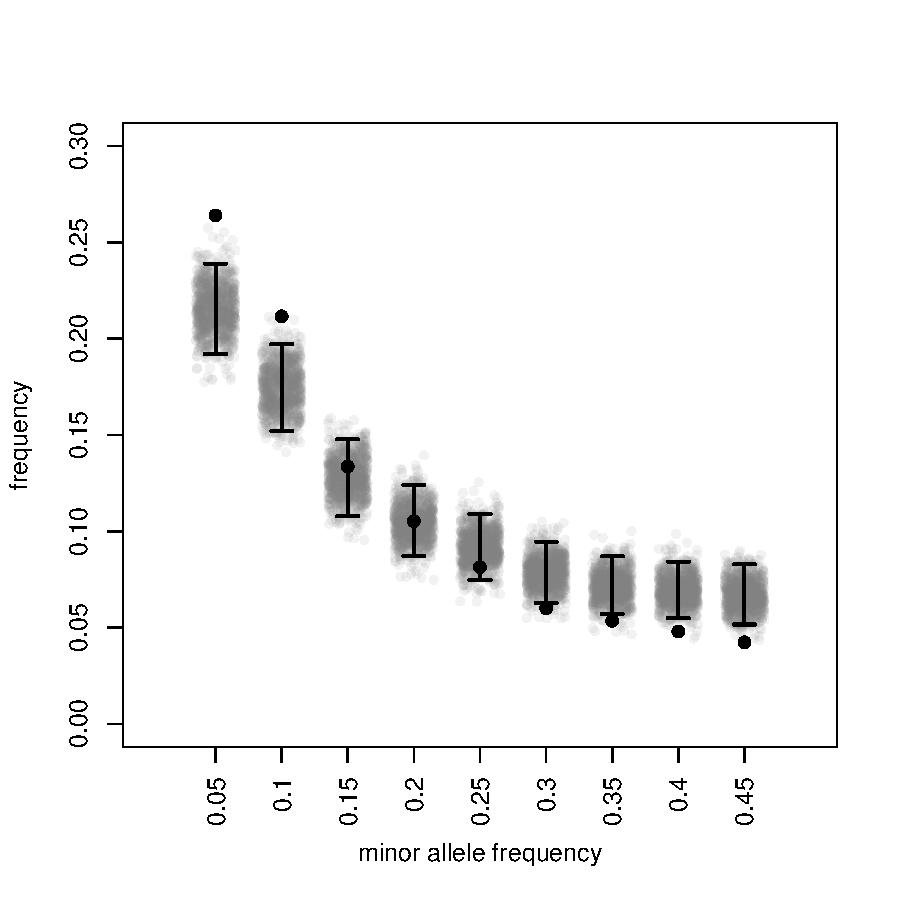
\includegraphics[width=\linewidth]{Ch3Sim}
    \caption{\textbf{The site frequency spectrum of aseQTLs when genes with SNPs showing ASE bias are removed from the analysis.} Red dots are frequencies of aseQTLs, gray dots are frequencies for permuted aseQTLs and black lines show 95\% confidence intervals. }
    \label{fig:3figS9}
\end{figure}


%% This adds a line for the Bibliography in the Table of Contents.
\addcontentsline{toc}{chapter}{Bibliography}
%% *** Set the bibliography style. ***
%% (change according to your preference/requirements)
%\bibliographystyle{natbib}
%% *** Set the bibliography file. ***
%% ("thesis.bib" by default; change as needed)
\bibliography{chapter3}
\bibliographystyle{ecology_letters2}

%% *** NOTE ***
%% If you don't use bibliography files, comment out the previous line
%% and use \begin{thebibliography}...\end{thebibliography}.  (In that
%% case, you should probably put the bibliography in a separate file and
%% `\include' or `\input' it here).

\end{document}
